\documentclass[usenatbib]{mnras}
\usepackage[T1]{fontenc}
\usepackage{inputenc}
\usepackage{graphicx}
\usepackage{grffile}
\usepackage{longtable}
\usepackage{wrapfig}
\usepackage{rotating}
\usepackage[normalem]{ulem}
\usepackage{amsmath}
\usepackage{textcomp}
\usepackage{amssymb}
\usepackage{capt-of}
\usepackage{hyperref}
\usepackage{rotating}
\usepackage{natbib}
\usepackage{caption}
\usepackage{subcaption}
\usepackage{varioref}
\usepackage{pdflscape}
\usepackage{bm}
\usepackage{pgfplots}
\usepackage{pgf}
\usepackage[nameinlink, capitalize, noabbrev]{cleveref}

\captionsetup{compatibility=false}
\usepgfplotslibrary{groupplots,dateplot}
\usetikzlibrary{patterns,shapes.arrows}
\pgfplotsset{compat=newest}
\usepackage{dsfont}
\usepackage{xcolor}
\usepackage{listings}

\DeclareMathOperator{\TopHat}{TH}
\DeclareMathOperator{\CDF}{CDF}

\author[A. Petrosyan and W. Handley]{
  Aleksandr Petrosyan,$^{1}$
  William James Handley, $^{2}$
  \\
  $^{1}$Cavendish Laboratory, University of Cambridge\\
  $^{2}$Kavli Institute of Astronomy, University of Cambridge
}
\date{\today}
\title[Accelerated Nested Sampling]{Accelerated nested sampling in the context of cosmological parameter estimation}
\hypersetup{
 pdftitle={Accelerated nested sampling in context of cosmological parameter estimation},
 pdflang={English}}
\crefname{Option}{Option}{Options}
\crefname{Property}{Property}{Properties}

\newcommand{\TODO}{\textbf{TODO}}

\begin{document}
\newpage
\thispagestyle{plain} % empty

\maketitle
\begin{abstract}
  By extending previous work, we have found a method of using
  intuitive proposals with nested sampling to improve performance,
  accuracy and precision, called consistent posterior
  repartitioning. We have also developed a prescription called
  stochastic isometric mixture, of combining several intuitive
  proposals into a single model. This prescription allows nested
  sampling to make use of the most representative of the proposal
  priors. As a consequence, the sampling is hardened against prior
  imprinting, while also retaining most of its performance and
  accuracy. We demonstrate this by comparing full cosmological
  parameter estimations performed with the inference package
  \texttt{Cobaya} utilising the module \texttt{CLASS}, with and
  without our modifications. We demonstrate a run-time reduction in
  CSD3 Skylake compute-hours by a factor of \(20\), accompanied with
  increased precision. When precision normalised, the predicted
  performance uplift is by three orders of magnitude.  The real-world
  performance uplift is such that cosmological inference was performed
  with a net precision gain on a personal computer within two days,
  provided a well-tuned proposal distribution. The findings are
  systematised, such that inference techniques that are similar to
  nested sampling in benefiting from our methods, can be
  identified. The scope of the findings suggests multiple improvements
  and an evolution of nested sampling.
\end{abstract}

\begin{keywords}
Bayesian inference --- automated posterior repartitioning --- nested sampling --- cosmology: miscellaneous --- methods: statistical --- methods: data analysis
\end{keywords}

\section{Introduction}\label{sec:org14413d7}

The standard model of the universe and its evolution in modern
cosmology is the \(\Lambda\)CDM model \citep{Condon2018}, so named
after the main components of the universe: the cosmological constant
\(\Lambda\) and cold dark matter. It has six major
independent\footnote{there can be other equivalent parameter
  sextuplets. } parameters: the physical baryon density
\(\Omega_\mathrm{b}h^{2}\); the physical (cold) dark matter density
\(\Omega_\mathrm{c}h^{2}\); the angular parameter
\(100\theta_\mathrm{s}\); re-ionisation optical depth
\(\tau_\text{reio}\); power spectrum slope \(n_\mathrm{s}\) and
amplitude \(\ln (10^{10}A_\mathrm{s})\) \citep{Cosmology}.

The task of the present study is to develop better tools for
evaluating the agreement of our observations from the Planck mission
with \(\Lambda\)CDM, estimating the parameters in the process. In the
language of Bayesian statistics\footnote{See \cite{xkcd} for
  comparison to frequentist statistics.}, our goal is efficient
Bayesian inference. 

While said inference can be executed analytically in principle, it is
often intractable. Multiple numerical algorithms exist to perform
Bayesian inference: Metropolis-Hastings \citep{Metropolis} in
conjunction with the Gibbs sampler \citep{Metropolis-Hastings-Gibbs};
Hybrid (Hamiltonian) Monte Carlo \citep{1701.02434,Duane_1987}, and
nested sampling \citep{Skilling2006}. Most inference methods can
benefit from proposals, so much so that these proposals are often
provided with the Cosmological inference packages
\citep{cobaya}. Nested sampling is the exception, because it does not
take proposals as separate input, and using them as priors may
adversely affect the results. We have found a prescription for
incorporating proposals safely: reducing the run-time, increasing the
precision, while assuaging if not eliminating the aforementioned
adverse effects.

\begin{table}
  \centering
  \caption{A non-exhaustive list of major implementations of nested sampling.}
  \begin{tabular}{lr}
    \textbf{Name} & \textbf{Publication}\\
    \hline
    \texttt{MultiNest} & \cite{Feroz2009MultiNestAE} \\
    \texttt{PolyChord} & \cite{polychord} \\
    \texttt{nestle} & \cite{nestle} \\
    \texttt{dyNesty} & \cite{Speagle_2020}
  \end{tabular}

\end{table}

We achieve this end by extending \emph{automatic power posterior
  re-partitioning} \citep{chen-ferroz-hobson}. The issues arising from
improper usage of proposals as priors, are a variant of the problem of
\emph{unrepresentative priors} that we shall discuss in
\cref{sec:autopr}. Hence, we find that posterior re-partitioning can
be used to mitigate prior imprints. We found multiple extensions of
posterior re-partitioning, with different trade-offs and potential.
From these extensions we have identified a combination that can
provide significantly better results: performance, accuracy,
precision, convenience, stability and imprint mitigation.

In the following section, we shall provide a brief primer on Bayesian
inference and nested sampling, followed by an exploration of work by
\cite{chen-ferroz-hobson}. All work is our own from the third section
onward, which includes the mathematical framework of consistent
partitions, a few examples\footnote{We present only a small subset of
  consistent partitions designed during the project. }, along with
descriptions of the underlying mechanism. We dedicate the final
sections to practical demonstrations and a few suggested applications
of our work.

\section{Theoretical background}\label{sec:orge6061a4}
In this section we summarise previous work, outlining the key
elements of Bayesian inference \citep{jeffreys2010scientific} and
automatic posterior repartitioning \citep{chen-ferroz-hobson}. 
\subsection{Bayesian inference}\label{sec:primer}

Hypothesis testing in Bayesian statistics requires said hypothesis to
be formulated in terms of conditional probabilities, organising
information in the following way.

A model \({\cal M}\) of a physical process, is parameterised by
\(\bm{\theta} = (\theta_{1}, \theta_{2}, \ldots , \theta_{n})\).  New
empirical observations of said process are encapsulated in the
\textbf{\emph{dataset}} \(\mathfrak{D}\).  The
\emph{\textbf{likelihood}} ${\cal L}$ of the parameters $\bm{\theta}$
is the probability of observing \(\mathfrak{D}\), conditional on the
configuration $\bm{\theta}$ and the model ${\cal M}$.  The prior
\(\pi(\bm{\theta})\) is the probability of $\bm{\theta}$ assuming
${\cal M}$. It can be obtained from both previous datasets as well as
constraints inherent to the model. The posterior is a probability of
$\bm{\theta}$ that is conditional on ${\cal M}$ and the dataset
${\mathfrak D}$. The locus of all $\bm{\theta}$ for which the prior is
both defined and non-zero defines the \textbf{\emph{prior space}}
$\Psi$. Finally, the \textbf{\emph{evidence}} is the probability of
the data \({\mathfrak D}\) assuming the model.

The interactions of probabilities of \cref{tab:defs} is governed by
\citeauthor{1763}'s theorem:
\begin{equation}\label{eq:bayes} 
 {\cal L}(\bm{\theta}) \times \pi (\bm{\theta}) = {\cal Z} \times {\cal P} (\bm{\theta}).  
\end{equation}

Bayesian inference is the process of reconciling the model ${\cal M}$
represented in ${\cal L}$ and $\pi$, with observations
\(\mathfrak{D}\) represented in ${\cal L}$. A numerical algorithm that
obtains ${\cal Z}$ and ${\cal P}$ from $\pi$ and ${\cal L}$, is called
a \textbf{\emph{sampling algorithm}} or \textbf{\emph{sampler}}.

The convenient representation of $\pi$ and ${\cal L}$ depends on the
particulars of the sampler. For \textbf{\emph{nested sampling}}
(e.g. \texttt{PolyChord}, \texttt{MultiNest}) we delineate them
indirectly: with the logarithm of the likelihood probability-density
function \(\ln \cal L (\bm{\theta})\), and \textbf{\emph{prior
    quantile}} \(C\{\pi\}(\bm{\theta})\). The latter is a coordinate
transformation $C: \bm{u} \mapsto \bm{\theta}$ that maps a uniform
distribution of $\bm{u}$ in a unit hypercube to $\pi(\bm{\theta})$ in
$\Psi$. It is often obtained by inverting the cumulative distribution
function of the prior.

\begin{table}
  \caption{Definitions of main quantities in Bayesian inference.   \label{tab:defs}}
\centering
\begin{tabular}{llr}
\textbf{\textbf{Term}} & \textbf{\textbf{Symbol}} & \textbf{\textbf{Definition}}\\
\hline
  Prior  & \(\pi(\bm{\theta})\) & \(P ( \bm{\theta}  \vert {\cal M})\) \\
  Likelihood  & \({\cal L}(\bm{\theta})\) & \(P ( \bm{\mathfrak{D}} \vert \bm{\theta} \cap {\cal M})\) \\
  Posterior  & \({\cal P}(\bm{\theta})\) & \(P ( \bm{\theta} \vert \bm{\mathfrak{D}} \cap {\cal M})\) \\
Evidence & \({\cal Z}\) & \(P ( \bm{\mathfrak{D}} \vert {\cal M})\) \\
\end{tabular}
\end{table}


For \citeauthor{1763}' theorem holds, on the set intersection of the
domains of all probability density functions. Let \(D(f)\) denote the
domain of the probability density function \(f\), i.e.~where \(f\) is
both defined and \textbf{non-zero}. Hence
\begin{equation}
  D \{ \pi \} \cap D \{ {\cal L} \} = D \{ {\cal P} \} \subset \Psi,
\end{equation} 
meaning the inference is possible only on a subset of the domain of
prior and likelihood.\label{domain-discussion}

For each choice of ${\cal L}$ and $\pi$, there is a unique choice of
${\cal Z}$ and ${\cal P}$; equivalently they represent the same unique
model ${\cal M}$, or partition it consistently. That correspondence is
\emph{surjective}, but not \emph{injective}: many choices of
\({\cal L}(\bm{\theta})\) and \(\pi (\bm{\theta})\) may correspond to
the same \( {\cal P} (\bm{\theta})\) and \({\cal Z}\)
\citep{chen-ferroz-hobson}. This remark is the cornerstone of our
optimisation.

\subsection{Nested Sampling}\label{sec:org36366f8}

${\cal P}$ is a probability, therefore normalised, which combined with
\cref{eq:bayes} yields
\begin{equation}
  \label{eq:def-z}
  {\cal Z} = \int_{\Psi} {\cal L}(\bm{\theta}) \pi(\bm{\theta}) d\bm{\theta}. 
\end{equation}
Thus, \citeauthor{1763}'s theorem reduces parameter estimation ---
obtaining ${\cal P}$ from $\pi$ and ${\cal L}$, to
integration~\citep{bayes-integration}. The naïve approach to obtain
\({\cal Z}\) of uniformly rasterising \(\Psi\) is intractable for
hypotheses with \(O(30)\) parameters
\citep{Caflisch_1998}. Integration is usually performed using Monte
Carlo techniques, such as nested sampling.

The following is a short description of nested sampling
\citep{Skilling2006}. We begin, by picking \(n_\text{live}\)
\textbf{\emph{live points}} at random in $\Psi$. During each
subsequent iteration, the point with the lowest likelihood is declared
\emph{\textbf{dead}}, and another live point $\bm{\theta}\in\Psi$ is
taken with a higher likelihood, based on the prior $\pi$ and an
implementation-dependent principle. Live points are thus gradually
moved into regions of high likelihood. By tracking their locations and
likelihoods, from a statistical argument we can approximate ${\cal Z}$
and its error for each iteration, and by \cref{eq:bayes},
${\cal P}(\bm{\theta})$. We continue until a pre-determined fraction
of the evidence associated to $\Psi$ remains unaccounted for.

Not all parameter inference methods require obtaining ${\cal Z}$. Some
methods, such as Hamiltonian Monte-Carlo \citep{1701.02434}, allow
obtaining a normalised ${\cal P}$ directly. For such approaches, any
consistent specification of $\pi$ and ${\cal L}$ will lead to
identically the same posterior, barring numerical errors. This is also
true of methods that evaluate ${\cal Z}$ exactly. However, nested
sampling allows uncertainty in ${\cal Z}$, which is controlled by
$\pi$ and ${\cal L}$. Thus, nested sampling, unlike,
e.g.~Metropolis-Hastings \citep{Metropolis-Hastings-Gibbs} is
sensitive to the concrete definitions of prior and likelihood. While
many choices of $\pi$ and ${\cal L}$ correspond to the same ${\cal P}$
and ${\cal Z}$, the errors and nested sampling's time complexity are
dependent on the specification of $\pi$
\citep{Skilling2006}. Specifically, more informative priors are
preferable.

A probability density function \(f(\bm{\theta})\) is said to be more
\emph{\textbf{informative}} than \(g(\bm{\theta})\) if:
\begin{equation}
  \label{eq:informative}
  {\cal D}\{ f, g \} > {\cal D}\{ g, f\}.
\end{equation}
This also highlights, that Kullback-Leibler divergence is not a metric
on the space of distributions. However, being asymmetric lends itself
well to considerations where such an asymmetry is natural: e.g.~priors
are not equivalent to posteriors, one comes after the other, and so
${\cal D}$ can be used to quantify the ``surprise'' information
obtained during inference.

The time complexity $T$ of nested sampling is
\begin{equation}\label{eq:complexity}
  T \propto  n_\text{live}\  \langle {\cal T}\{{\cal L}(\bm{\theta})\} \rangle \ \langle  {\cal N}\{{\cal L}(\bm{\theta}) \}, 
\end{equation}
where ${\cal T}\{f(\bm{\theta})\}$ is the time complexity of
evaluating $f(\bm{\theta})$ and ${\cal N}\{f(\bm{\theta})\}$ --- the
quantity of such evaluations. Reducing $n_\text{live}$ reduces the
resolution of nested sampling, while
$ {\cal T}\{{\cal L}(\bm{\theta})\}$ is model-dependent. We can,
however, reduce the number of likelihood evaluations, by providing a
more informative prior. However, there is an associated risk, which we
shall address later.

An important quantity for measuring the correctness of the obtained
posterior is the \textbf{\emph{Kullback-Leibler divergence}} ${\cal D}$
\citep{Kullback_1951}. For probability distributions
\(f(\bm{\theta})\) and \(g(\bm{\theta})\), it is defined as:
\begin{equation}
  \label{eq:kl-def}
  {\cal D}\{f, g \} = \int_{\Psi}f(\bm{\theta}) \ln \frac{f(\bm{\theta})}{g(\bm{\theta})} d \bm{\theta}.
\end{equation}
It is a pre-metric on the space of probability distributions: it is
nil if and only if $f(\bm{\theta}) = g(\bm{\theta})$, (albeit not
symmetric) which is convenient for defining a representation
hierarchy. The statement: $f$ represents $g$ better than $h$ is
equivalent to
\begin{equation}
  \label{eq:hierarchy}
  {\cal D}\{f, g\} < {\cal D}\{h, g\}.
\end{equation}
Specifically, distribution $h$ is said to be unrepresentative of $g$
if a uniform distribution $f$ represents $g$ better than $h$.

Choosing the correct representations of ${\cal P}$ and $\pi$ is
crucial for nested sampling's correctness and performance. For
example, assuming the same likelihood, if $\pi_{0}$ and $\pi_{1}$ are
equally informative, but $\pi_{0}$ is more representative of
${\cal P}$, then the inference with $\pi_{0}$ will terminate more
quickly than with $\pi_{1}$, (more accurate, also).

Similarly, if $\pi_{1}$ is more informative than $\pi_{2}$, but
equally as representative, nested sampling will terminate with
$\pi_{1}$ faster than with $\pi_{2}$, and the result will be more
precise. In detail, if \(\pi_{1} (\bm{\theta})\) is more similar to
\( {\cal P} (\bm{\theta})\), then points drawn with PDF
\(\pi_{1} (\bm{\theta})\) are more likely to lie in $\bm{\theta}$
regions of high \( {\cal P} (\bm{\theta})\), leading to fewer
iterations.

Posteriors ${\cal P}_{1}$ and ${\cal P}_{2}$ obtained with the priors
$\pi_{1}$ and $\pi_{2}$ are different, because of \cref{eq:bayes}. In
fact, the posterior ${\cal P}_{1}$ will be more informative than
${\cal P}_{2}$, and more similar to $\pi_{1}$. This effect we call
\textbf{\emph{prior imprinting}}.


Imprinting is desirable if the informative prior $\pi_{1}$ is the
result of inference over another dataset. Nonetheless, imprinting
limits the information obtainable from \(\mathfrak{D}\). There is a
considerable risk of getting no usable data from the inference, which
makes one prefer uniform priors even when more information is
available. 

The problem is exasperated in case of proposals. The issue is that the
algorithm has no room to consult the proposal distributions outside of
the prior. Using a prior taken out of ``thin air'', with nested
sampling is a recipe for disaster. However, in the next section we
shall discuss how one can mitigate these issues, and use a proposal as
an aspect of a prior.


\subsection{Power posterior repartitioning}\label{sec:autopr}
From this section onward we shall adopt the following notation. $\pi$
and ${\cal L}$ with similar annotations (index, diacritics), belong to
the same specification of the model. Models using the uniform prior
are special, in that they obtain the most accurate posterior and
evidence. They are represented with an over-bar (the plot of a uniform
prior in 1D is a horizontal line). Hats delineate the consistent
partitions, that incorporate the proposal (the hat represents the
peak(s) often present in informative proposals).

We are working under the assumption that $\pi(\bm{\theta})$ is an
informative, unrepresentative prior. We want to obtain correct
posterior $\bar{\cal P}$ but without using a uniform, universally
representative reference prior $\bar{\pi}$, because it is often the
least informative. To avoid loss of precision and mitigate prior
imprinting, \cite{chen-ferroz-hobson} have proposed introducing the
parameter \(\beta\) to control the breadth of the informative prior:
\begin{equation}
  \label{eq:autopr-prior}
  \hat{\pi}(\bm{\bm{\theta}};\beta) = \cfrac{\pi(\bm{\theta})^{\beta}}{Z(\beta)\{\pi\}},
\end{equation}
(see \cref{fig:ppr}) where \(Z(\beta)\{\pi\}\) --- a functional of
\(\pi (\bm{\theta})\) is a normalisation factor for
\( {\cal P} (\bm{\theta})\), i.e.
\begin{equation}
  Z(\beta)\{\pi\} = \int_{\Psi} \pi(\bm{\bm{\theta}})^{\beta}d\bm{\bm{\theta}}.
\end{equation}
In their prescription, the likelihood changes to
\begin{equation}
  \hat{\cal L}(\bm{\theta}; \beta) = {\cal L}(\bm{\theta}) Z(\beta)\{\pi\} \cdot \pi^{1-\beta}(\bm{\theta}).
\end{equation}
The new parameter $\beta$ is treated as any other non-derived
parameter of the original theory.

\begin{figure}
 % This file was created by tikzplotlib v0.9.1.
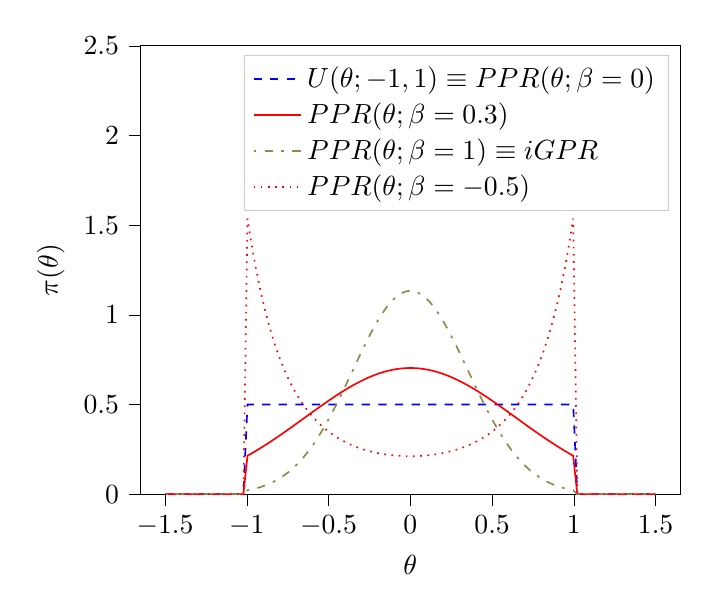
\begin{tikzpicture}

\begin{axis}[
legend cell align={left},
legend style={fill opacity=0.8, draw opacity=1, text opacity=1, draw=white!80!black},
tick align=outside,
tick pos=left,
x grid style={white!69.0196078431373!black},
xlabel={\(\displaystyle \theta\)},
xmin=-1.65, xmax=1.65,
xtick style={color=black},
y grid style={white!69.0196078431373!black},
ylabel={\(\displaystyle \pi(\theta)\)},
ymin=0, ymax=2.5,
ytick style={color=black}
]
\addplot [semithick, blue, dashed]
table {%
-1.5 0
-1.47478991596639 0
-1.44957983193277 0
-1.42436974789916 0
-1.39915966386555 0
-1.37394957983193 0
-1.34873949579832 0
-1.32352941176471 0
-1.29831932773109 0
-1.27310924369748 0
-1.24789915966387 0
-1.22268907563025 0
-1.19747899159664 0
-1.17226890756303 0
-1.14705882352941 0
-1.1218487394958 0
-1.09663865546218 0
-1.07142857142857 0
-1.04621848739496 0
-1.02100840336134 0
-0.995798319327731 0.5
-0.970588235294118 0.5
-0.945378151260504 0.5
-0.920168067226891 0.5
-0.894957983193277 0.5
-0.869747899159664 0.5
-0.84453781512605 0.5
-0.819327731092437 0.5
-0.794117647058823 0.5
-0.76890756302521 0.5
-0.743697478991597 0.5
-0.718487394957983 0.5
-0.69327731092437 0.5
-0.668067226890756 0.5
-0.642857142857143 0.5
-0.617647058823529 0.5
-0.592436974789916 0.5
-0.567226890756303 0.5
-0.542016806722689 0.5
-0.516806722689076 0.5
-0.491596638655462 0.5
-0.466386554621849 0.5
-0.441176470588235 0.5
-0.415966386554622 0.5
-0.390756302521008 0.5
-0.365546218487395 0.5
-0.340336134453781 0.5
-0.315126050420168 0.5
-0.289915966386554 0.5
-0.264705882352941 0.5
-0.239495798319328 0.5
-0.214285714285714 0.5
-0.189075630252101 0.5
-0.163865546218487 0.5
-0.138655462184874 0.5
-0.113445378151261 0.5
-0.088235294117647 0.5
-0.0630252100840336 0.5
-0.03781512605042 0.5
-0.0126050420168067 0.5
0.0126050420168067 0.5
0.0378151260504203 0.5
0.0630252100840336 0.5
0.0882352941176472 0.5
0.113445378151261 0.5
0.138655462184874 0.5
0.163865546218487 0.5
0.189075630252101 0.5
0.214285714285714 0.5
0.239495798319328 0.5
0.264705882352941 0.5
0.289915966386555 0.5
0.315126050420168 0.5
0.340336134453782 0.5
0.365546218487395 0.5
0.390756302521008 0.5
0.415966386554622 0.5
0.441176470588235 0.5
0.466386554621849 0.5
0.491596638655462 0.5
0.516806722689076 0.5
0.542016806722689 0.5
0.567226890756303 0.5
0.592436974789916 0.5
0.617647058823529 0.5
0.642857142857143 0.5
0.668067226890756 0.5
0.69327731092437 0.5
0.718487394957983 0.5
0.743697478991597 0.5
0.76890756302521 0.5
0.794117647058823 0.5
0.819327731092437 0.5
0.844537815126051 0.5
0.869747899159664 0.5
0.894957983193277 0.5
0.920168067226891 0.5
0.945378151260504 0.5
0.970588235294118 0.5
0.995798319327731 0.5
1.02100840336134 0
1.04621848739496 0
1.07142857142857 0
1.09663865546218 0
1.1218487394958 0
1.14705882352941 0
1.17226890756303 0
1.19747899159664 0
1.22268907563025 0
1.24789915966387 0
1.27310924369748 0
1.29831932773109 0
1.32352941176471 0
1.34873949579832 0
1.37394957983193 0
1.39915966386555 0
1.42436974789916 0
1.44957983193277 0
1.47478991596639 0
1.5 0
};
\addlegendentry{$U(\theta; -1, 1) \equiv PPR(\theta; \beta=0)$}
\addplot [semithick, red]
table {%
-1.5 0
-1.47478991596639 0
-1.44957983193277 0
-1.42436974789916 0
-1.39915966386555 0
-1.37394957983193 0
-1.34873949579832 0
-1.32352941176471 0
-1.29831932773109 0
-1.27310924369748 0
-1.24789915966387 0
-1.22268907563025 0
-1.19747899159664 0
-1.17226890756303 0
-1.14705882352941 0
-1.1218487394958 0
-1.09663865546218 0
-1.07142857142857 0
-1.04621848739496 0
-1.02100840336134 0
-0.995798319327731 0.213997817612381
-0.970588235294118 0.227114237828303
-0.945378151260504 0.240667220043335
-0.920168067226891 0.254640269643853
-0.894957983193277 0.269013944947124
-0.869747899159664 0.283765808073716
-0.84453781512605 0.298870396474599
-0.819327731092437 0.314299216545356
-0.794117647058823 0.330020760597652
-0.76890756302521 0.346000548271141
-0.743697478991597 0.362201193258465
-0.718487394957983 0.378582495983783
-0.69327731092437 0.395101562623435
-0.668067226890756 0.411712950588459
-0.642857142857143 0.428368840305768
-0.617647058823529 0.445019232841112
-0.592436974789916 0.461612172606143
-0.567226890756303 0.478093994087889
-0.542016806722689 0.494409591235828
-0.516806722689076 0.510502707843814
-0.491596638655462 0.526316246975685
-0.466386554621849 0.541792597208828
-0.441176470588235 0.556873973213705
-0.415966386554622 0.571502767953309
-0.390756302521008 0.585621913578992
-0.365546218487395 0.599175247921439
-0.340336134453781 0.612107883331366
-0.315126050420168 0.624366574516491
-0.289915966386554 0.635900081952001
-0.264705882352941 0.64665952741297
-0.239495798319328 0.656598738190246
-0.214285714285714 0.665674576606966
-0.189075630252101 0.673847251551064
-0.163865546218487 0.681080608879363
-0.138655462184874 0.687342397729793
-0.113445378151261 0.692604509998021
-0.088235294117647 0.696843190490911
-0.0630252100840336 0.700039215558481
-0.03781512605042 0.702178038324864
-0.0126050420168067 0.703249898983013
0.0126050420168067 0.703249898983013
0.0378151260504203 0.702178038324864
0.0630252100840336 0.700039215558481
0.0882352941176472 0.696843190490911
0.113445378151261 0.692604509998021
0.138655462184874 0.687342397729793
0.163865546218487 0.681080608879363
0.189075630252101 0.673847251551064
0.214285714285714 0.665674576606966
0.239495798319328 0.656598738190246
0.264705882352941 0.64665952741297
0.289915966386555 0.635900081952001
0.315126050420168 0.624366574516491
0.340336134453782 0.612107883331366
0.365546218487395 0.599175247921439
0.390756302521008 0.585621913578992
0.415966386554622 0.571502767953309
0.441176470588235 0.556873973213705
0.466386554621849 0.541792597208828
0.491596638655462 0.526316246975685
0.516806722689076 0.510502707843814
0.542016806722689 0.494409591235828
0.567226890756303 0.478093994087889
0.592436974789916 0.461612172606143
0.617647058823529 0.445019232841112
0.642857142857143 0.428368840305768
0.668067226890756 0.41171295058846
0.69327731092437 0.395101562623435
0.718487394957983 0.378582495983783
0.743697478991597 0.362201193258465
0.76890756302521 0.346000548271141
0.794117647058823 0.330020760597652
0.819327731092437 0.314299216545355
0.844537815126051 0.298870396474599
0.869747899159664 0.283765808073716
0.894957983193277 0.269013944947124
0.920168067226891 0.254640269643852
0.945378151260504 0.240667220043335
0.970588235294118 0.227114237828303
0.995798319327731 0.213997817612381
1.02100840336134 0
1.04621848739496 0
1.07142857142857 0
1.09663865546218 0
1.1218487394958 0
1.14705882352941 0
1.17226890756303 0
1.19747899159664 0
1.22268907563025 0
1.24789915966387 0
1.27310924369748 0
1.29831932773109 0
1.32352941176471 0
1.34873949579832 0
1.37394957983193 0
1.39915966386555 0
1.42436974789916 0
1.44957983193277 0
1.47478991596639 0
1.5 0
};
\addlegendentry{$PPR(\theta; \beta=0.3)$}
\addplot [semithick, yellow!50!black, dash pattern=on 1pt off 3pt on 3pt off 3pt]
table {%
-1.5 0
-1.47478991596639 0
-1.44957983193277 0
-1.42436974789916 0
-1.39915966386555 0
-1.37394957983193 0
-1.34873949579832 0
-1.32352941176471 0
-1.29831932773109 0
-1.27310924369748 0
-1.24789915966387 0
-1.22268907563025 0
-1.19747899159664 0
-1.17226890756303 0
-1.14705882352941 0
-1.1218487394958 0
-1.09663865546218 0
-1.07142857142857 0
-1.04621848739496 0
-1.02100840336134 0
-0.995798319327731 0.0214724142964886
-0.970588235294118 0.0261816854177165
-0.945378151260504 0.0317618800741448
-0.920168067226891 0.0383359898858045
-0.894957983193277 0.0460361547091755
-0.869747899159664 0.0550026075477869
-0.84453781512605 0.065382179833744
-0.819327731092437 0.0773263287734615
-0.794117647058823 0.0909886594168491
-0.76890756302521 0.106521928411203
-0.743697478991597 0.124074533966699
-0.718487394957983 0.143786517124182
-0.69327731092437 0.165785122499698
-0.668067226890756 0.190179991583716
-0.642857142857143 0.217058087477864
-0.617647058823529 0.246478475540006
-0.592436974789916 0.27846710849647
-0.567226890756303 0.313011785770707
-0.542016806722689 0.350057473625004
-0.516806722689076 0.38950218380086
-0.491596638655462 0.431193612377642
-0.466386554621849 0.474926736461832
-0.441176470588235 0.520442553285407
-0.415966386554622 0.567428123929624
-0.390756302521008 0.615518052248804
-0.365546218487395 0.664297489193931
-0.340336134453781 0.713306704691472
-0.315126050420168 0.762047215088407
-0.289915966386554 0.809989395961805
-0.264705882352941 0.856581450226966
-0.239495798319328 0.90125954265622
-0.214285714285714 0.943458856978025
-0.189075630252101 0.982625283491455
-0.163865546218487 1.01822740626125
-0.138655462184874 1.04976843177719
-0.113445378151261 1.07679768730853
-0.088235294117647 1.09892131828878
-0.0630252100840336 1.11581183044719
-0.03781512605042 1.12721615381797
-0.0126050420168067 1.13296195118377
0.0126050420168067 1.13296195118377
0.0378151260504203 1.12721615381797
0.0630252100840336 1.11581183044719
0.0882352941176472 1.09892131828878
0.113445378151261 1.07679768730853
0.138655462184874 1.04976843177719
0.163865546218487 1.01822740626125
0.189075630252101 0.982625283491455
0.214285714285714 0.943458856978025
0.239495798319328 0.90125954265622
0.264705882352941 0.856581450226966
0.289915966386555 0.809989395961804
0.315126050420168 0.762047215088407
0.340336134453782 0.713306704691471
0.365546218487395 0.664297489193931
0.390756302521008 0.615518052248804
0.415966386554622 0.567428123929624
0.441176470588235 0.520442553285407
0.466386554621849 0.474926736461831
0.491596638655462 0.431193612377642
0.516806722689076 0.38950218380086
0.542016806722689 0.350057473625004
0.567226890756303 0.313011785770707
0.592436974789916 0.27846710849647
0.617647058823529 0.246478475540006
0.642857142857143 0.217058087477864
0.668067226890756 0.190179991583716
0.69327731092437 0.165785122499698
0.718487394957983 0.143786517124182
0.743697478991597 0.124074533966699
0.76890756302521 0.106521928411203
0.794117647058823 0.0909886594168492
0.819327731092437 0.0773263287734614
0.844537815126051 0.065382179833744
0.869747899159664 0.0550026075477869
0.894957983193277 0.0460361547091755
0.920168067226891 0.0383359898858044
0.945378151260504 0.0317618800741447
0.970588235294118 0.0261816854177165
0.995798319327731 0.0214724142964886
1.02100840336134 0
1.04621848739496 0
1.07142857142857 0
1.09663865546218 0
1.1218487394958 0
1.14705882352941 0
1.17226890756303 0
1.19747899159664 0
1.22268907563025 0
1.24789915966387 0
1.27310924369748 0
1.29831932773109 0
1.32352941176471 0
1.34873949579832 0
1.37394957983193 0
1.39915966386555 0
1.42436974789916 0
1.44957983193277 0
1.47478991596639 0
1.5 0
};
\addlegendentry{$PPR(\theta; \beta=1) \equiv iGPR$}
\addplot [semithick, red, dotted]
table {%
-1.5 0
-1.47478991596639 0
-1.44957983193277 0
-1.42436974789916 0
-1.39915966386555 0
-1.37394957983193 0
-1.34873949579832 0
-1.32352941176471 0
-1.29831932773109 0
-1.27310924369748 0
-1.24789915966387 0
-1.22268907563025 0
-1.19747899159664 0
-1.17226890756303 0
-1.14705882352941 0
-1.1218487394958 0
-1.09663865546218 0
-1.07142857142857 0
-1.04621848739496 0
-1.02100840336134 0
-0.995798319327731 1.53654182295763
-0.970588235294118 1.39150901596467
-0.945378151260504 1.2633733862193
-0.920168067226891 1.14995668929314
-0.894957983193277 1.04938609279887
-0.869747899159664 0.960048526345581
-0.84453781512605 0.880552241346354
-0.819327731092437 0.809694387549735
-0.794117647058823 0.746433618973658
-0.76890756302521 0.689866910897954
-0.743697478991597 0.639209908533683
-0.718487394957983 0.593780242449033
-0.69327731092437 0.552983340262401
-0.668067226890756 0.516300342142374
-0.642857142857143 0.483277792232245
-0.617647058823529 0.453518831646172
-0.592436974789916 0.426675663124867
-0.567226890756303 0.402443094391563
-0.542016806722689 0.380552998023537
-0.516806722689076 0.360769551323719
-0.491596638655462 0.342885141121307
-0.466386554621849 0.326716836373627
-0.441176470588235 0.312103346479094
-0.415966386554622 0.298902395834313
-0.390756302521008 0.286988455782277
-0.365546218487395 0.276250784038563
-0.340336134453781 0.266591729226135
-0.315126050420168 0.25792526452701
-0.289915966386554 0.250175719862309
-0.264705882352941 0.24327668660032
-0.239495798319328 0.237170072698339
-0.214285714285714 0.231805289519371
-0.189075630252101 0.227138554422647
-0.163865546218487 0.223132295685766
-0.138655462184874 0.219754648442412
-0.113445378151261 0.216979032169198
-0.088235294117647 0.214783801876271
-0.0630252100840336 0.213151966589964
-0.03781512605042 0.212070969997919
-0.0126050420168067 0.21153252928888
0.0126050420168067 0.21153252928888
0.0378151260504203 0.212070969997919
0.0630252100840336 0.213151966589964
0.0882352941176472 0.214783801876271
0.113445378151261 0.216979032169198
0.138655462184874 0.219754648442412
0.163865546218487 0.223132295685766
0.189075630252101 0.227138554422647
0.214285714285714 0.231805289519371
0.239495798319328 0.237170072698339
0.264705882352941 0.24327668660032
0.289915966386555 0.250175719862309
0.315126050420168 0.25792526452701
0.340336134453782 0.266591729226135
0.365546218487395 0.276250784038563
0.390756302521008 0.286988455782277
0.415966386554622 0.298902395834313
0.441176470588235 0.312103346479094
0.466386554621849 0.326716836373627
0.491596638655462 0.342885141121307
0.516806722689076 0.360769551323719
0.542016806722689 0.380552998023537
0.567226890756303 0.402443094391563
0.592436974789916 0.426675663124867
0.617647058823529 0.453518831646172
0.642857142857143 0.483277792232245
0.668067226890756 0.516300342142374
0.69327731092437 0.552983340262402
0.718487394957983 0.593780242449033
0.743697478991597 0.639209908533683
0.76890756302521 0.689866910897954
0.794117647058823 0.746433618973658
0.819327731092437 0.809694387549735
0.844537815126051 0.880552241346354
0.869747899159664 0.960048526345581
0.894957983193277 1.04938609279887
0.920168067226891 1.14995668929314
0.945378151260504 1.2633733862193
0.970588235294118 1.39150901596467
0.995798319327731 1.53654182295763
1.02100840336134 0
1.04621848739496 0
1.07142857142857 0
1.09663865546218 0
1.1218487394958 0
1.14705882352941 0
1.17226890756303 0
1.19747899159664 0
1.22268907563025 0
1.24789915966387 0
1.27310924369748 0
1.29831932773109 0
1.32352941176471 0
1.34873949579832 0
1.37394957983193 0
1.39915966386555 0
1.42436974789916 0
1.44957983193277 0
1.47478991596639 0
1.5 0
};
\addlegendentry{$PPR(\theta; \beta=-0.5)$}
\end{axis}

\end{tikzpicture}

 \caption{\label{fig:ppr} Demonstration of
   \(\hat{\pi}(\theta; \beta)\) for different values of \(\beta\) in
   one dimension. We've assumed that the original
   \( \pi (\bm{\theta})\) distribution is a truncated Gaussian,
   i.e.~zero outside the region \((-1, 1)\). Numerical instability,
   which manifests as changes in curvature at the boundaries
   exaggerated. The area under curves for different $\beta$ is
   normalised to unity as in \cref{eq:autopr-prior}. }
\end{figure}

Note, that
\({\cal L}(\bm{\theta})\pi (\bm{\theta}) = \hat{\cal L}(\bm{\theta})
\hat{\pi} (\bm{\theta})\) by construction. Thus, from \cref{eq:bayes}
the posterior and evidence corresponding to
\(\hat{\cal L}(\bm{\theta};\beta)\) and
\(\hat{\pi} (\bm{\theta};\beta)\) will be the same as
\( {\cal P} (\bm{\theta})\) and \({\cal Z}\), which correspond to the
original $\pi(\bm{\theta})$ and ${\cal L}(\bm{\theta})$.

If the informative prior \(\pi (\bm{\theta})\) is less representative
of the posterior \( \bar{\cal P} (\bm{\theta})\), error in
$\hat{\cal Z}$ is larger. Hence, while we don't violate
\cref{eq:bayes} directly, $\bar{\cal Z}$ can be more different from
${\cal Z}$ while remaining within margin of error, and similarly
${\cal P}(\bm{\theta}) \ne \bar{\cal P}(\bm{\theta})$. This is where
the new parameter comes into play. $\hat{\pi}$ may become
representative for some value of $\beta = \beta_{R}$. Values $\beta$
close to $\beta_{R}$ correlate with higher likelihoods, thus the
sampler prefers them. Hence, the system will converge to a state where
\( {\cal P} (\bm{\theta})\) is represented in
\(\hat{\pi} (\bm{\theta};\beta)\)\footnote{Technically we obtain
  \( \hat{\cal P} (\bm{\theta};\beta)\) which, when marginalised over
  $\beta$, yields
  \( {\cal P} (\bm{\theta}) = \int \hat{\cal P} (\bm{\theta};\beta) d
  \beta\) --- the correct posterior.}.  As a consequence, we reduced
the errors and obtained the same result as we would have with a less
informative but more representative prior.

\cite{chen-ferroz-hobson} dubbed this scheme \textbf{\emph{automatic
    power posterior repartitioning}} (PPR) because the choice of
$\beta\rightarrow\beta_{R}$ is automatic. It mitigates the loss
precision and thus accuracy for unrepresentative informative priors
$\pi$, by sacrificing performance.

\pagebreak[2]
\section{Theoretical discoveries}
\subsection{The trouble with proposals\label{sec:prejudice}}

Nested sampling is different from Metropolis-Hastings-Gibbs and many
other Markov-Chain Monte Carlo methods. Often, such algorithms are
designed with a separate input that is the proposal: an initial guess
that guides the algorithm towards the right answer.  For nested
sampling no such provisions are in place. The only location where such
information can be used is the prior.  Thus, to understand why one
can't use proposals directly, we must first address why informative
priors are avoided.

From \cref{eq:bayes}, we can see that changing only the prior $\pi$
necessarily leads to changes in both ${\cal P}$ and ${\cal Z}$. For
example if $\pi$ is a Gaussian centered at
$\bm{\theta}=\bm{\mu}_{\pi}$ and ${\cal L}$ is a Dirac
$\delta$-function peaked at $\bm{\theta}=\bm{\mu}_{{\cal L}}$, with
$\bm{\mu}_{\pi}$ sufficiently far from $\bm{\mu}_{{\cal L}}$ then the
posterior will necessarily have peaks at both $\bm{\mu}_{\pi}$ and
$\bm{\mu}_{{\cal L}}$. This is an example of prior imprinting and is a
necessary part of a Bayesian view of statistics. For a Bayesian, the
prior information is no less valuable than the information inferred
from the dataset \(\mathfrak{D}\), and the posterior represents
\emph{all} of our best knowledge.

The problem however, is the \emph{prejudiced sampler}. Because nested
sampling chooses live points with probability proportional to the
prior, the probability of a point being drawn from the likelihood peak
can be made arbitrarily small. In fact, if $\bm{\mu}_{{\cal L}}$ and
$\bm{\mu}_{\pi}$ are separated by more than five standard deviations
of the prior Gaussian, thirty million samples will be drawn from
$\bm{\mu}_{\pi}$ before a single point is drawn on the circle
containing $\bm{\theta} = \bm{\mu}_{{\cal L}}$.

An apt analogy can be drawn with the Venera-14 mission
\citep{siddiqi2018beyond}. Upon landing, due to a number of
unfortunate coincidences, the lander took its one and only measurement
of Venusian soil from one of its own lens caps. As a result, we have
obtained objectively correct information from Venus: a sample of an
object on its surface. However, the efficiency of said measurement of
the compressibility of Earth rubber leaves much to be desired. 

Before \cite{chen-ferroz-hobson} the best solution was to use a
uniform prior that included both $\bm{\mu}_{\pi}$ and
$\bm{\mu}_{{\cal L}}$. The computational cost of inference is so high
that the risk of gaining nothing from a dataset is untenable. Thus
discarding all prior information in hopes of inferring some from the
dataset is preferable to using the information in $\pi$. 

Thus, proposals are not even considered for use with nested sampling.
Since proposals may be crude approximations, we may obtain far worse
than no new information.  Any potential benefit in performance or
precision is far outweighed by the unreliable posterior.  We do,
however, have one method of mitigating these problems --- automatic
posterior repartitioning \citep{chen-ferroz-hobson}. In the following
sections we shall expand our arsenal of methods of avoiding these
pitfalls and incorporating proposals into nested sampling-based
inference.

\subsection{Intuitive proposals and accelerated convergence\label{sec:accelerating}}
Consider the following premise: we're given a model \({\cal M}\), for
which our prior $\pi$ is not the uniform
\(\bar{\pi}(\bm{\theta})\). So, usually from other %
sources, e.g.~other inferences, physical reasoning, etc,  we know that
\begin{equation}
  \pi (\bm{\theta}) = f(\bm{\theta}; \bm{\mu}, \bm{\Sigma}),
 \label{eq:bias}
\end{equation}
which is representative of the posterior
\(\bar{\cal P}(\bm{\theta})\). Here, the probability density function
$f$ is parameterised by \(\bm{\mu}\) in its location and
\(\bm{\Sigma}\) its breadth. In order to obtain the same result as one
would have with the less informative uniform prior
\(\bar{\pi}(\bm{\theta})\), one needs to correct the likelihood
${\cal L}$. Recall, that the reason why PPR obtains the same posterior
\( \bar{\cal P}(\bm{\theta})= \hat{\cal P}(\bm{\theta})\) as one would
have using \( \bar{\pi} (\bm{\theta}) = \text{Const.}\) is because
\( \hat{\cal L} (\bm{\theta};\beta)\) and
\( \hat{\pi} (\bm{\theta};\beta)\) are a \textbf{\emph{consistent
    (re)partitioning}} of \( \bar{\cal Z}\) and
\({\cal P}(\bm{\theta})\). That is:
\begin{equation}
  \label{eq:partitioning}
  \int_{\Psi} \hat{\cal L} (\hat{\bm{\theta}}) \hat{\pi} (\bm{\hat{\theta}}) d\hat{\bm{\theta}}  = \int_{\Psi}\bar{\pi} (\bm{\theta}) \bar{\cal L} (\bm{\theta}) d\bm{\theta} = \bar{\cal Z}, 
\end{equation}
where in the case of PPR
$\hat{\bm{\theta}} = (\theta_{1}, \theta_{2}, \ldots, \theta_{n},
\beta)$. \Cref{eq:partitioning} holds if
\begin{equation}
  \label{eq:partitioning-p}
  \hat{\cal L}(\bm{\theta};\beta) \hat{\pi}(\bm{\theta};\beta)  = \bar{\cal L}(\bm{\theta})\bar{\pi}(\bm{\theta}) 
\end{equation}
for all $\beta$, by \cref{eq:bayes}. Note that
\cite{chen-ferroz-hobson} have used \cref{eq:partitioning-p} as the
primary expression. Following their convention, we shall sometimes
refer to consistent partitions as posterior repartitioning, rather
than evidence repartitioning.

By using a more informative prior in thusly, we accelerates
convergence, because each iteration obtains a larger evidence
estimate, so fewer are needed to reach the termination point
(See~\cref{fig:benchmark}). There is a competing mechanism: the
evidence estimates accumulate fewer errors, so inference proceeds
longer before the precision loss triggers termination
(\cref{fig:higson}). Thus repartitioning reaches a more precise result
quicker. Of course the obtained precision can be sacrificed to further
accelerate inference. 

\subsubsection{Example: intuitive proposal posterior repartitioning}
Suppose that one has obtained the posterior \({\cal P}(\bm{\theta})\)
from a different inference, which could be nested sampling with a
uniform prior, or Hamiltonian Monte Carlo (or a theoretical
approximation). Thus,
\begin{subequations}
\begin{equation}
  \label{eq:iPPR}
 \hat{\pi}(\bm{\theta}) = f(\bm{\theta}, \bm{\mu}, \bm{\Sigma}) = {\cal P}(\bm{\theta}), 
\end{equation}
is an informative prior that represents our knowledge, but might not
represent the posterior. We call it an \textbf{\emph{(intuitive)
    proposal}}. However, we wish to avoid prejudicing the sampler and
use the (uniform) reference prior $\bar{\pi}(\bm{\theta})$, with
reference likelihood $\bar{\cal L}(\bm{\theta})$.

To obtain with $\hat{\pi}(\bm{\theta})$ the same posterior and
evidence as one would have with $\bar{\pi}(\bm{\theta})$ and
$\bar{\cal L}(\bm{\theta})$, the partitioning of the (evidence) needs
to be \textbf{\emph{consistent}} with the reference. Specifically:
\begin{equation}
  \label{eq:ippr-l}
  \hat{\cal L}(\bm{\theta}) = \frac{\bar{\pi}(\bm{\theta}) \bar{\cal L}(\bm{\theta})}{ f(\bm{\theta}; \bm{\mu}, \bm{\Sigma})}.
\end{equation}
\end{subequations}
We call this scheme \textbf{\emph{intuitive proposal posterior\footnote{More
      accurately evidence repartitioning, which is equivalent in
      simple cases.} repartitioning}} (iPPR). It is the fastest
possible and the least robust consistent partitioning scheme. While we
have technically addressed the change in ${\cal P}$ due to a different
prior, we have not addressed the problem of $\hat{\pi}$ being
(potentially) unrepresentative of $\bar{\cal P}$. In the example
already considered in \cref{sec:prejudice}, we will have reduced prior
imprinting, but not all addressed the prejudice. The probability of
sampling from the true likelihood peak is still minuscule.  By
contrast, we have seen that automatic power posterior repartitioning
can mitigate both issues. What iPPR lacks, is a mechanism for
extending its representation. Rather than attempt a modification akin
to power partitioning, in \cref{sec:isomixtures} we shall provide this
mechanism as completely external to iPPR and unleash its potential.


\subsection{General automatic posterior repartitioning}\label{sec:gapr}

In this section, we look at the family of prescriptions similar to PPR
and iPPR called consistent partitioning. We note which schemes are
more useful for the task of accelerating nested sampling without
biasing the posterior. We begin by noting, that \Cref{eq:partitioning}
alone does not guarantee the correct posterior and evidence.

We shall consider a general consistent partitioning
\(\hat{\pi}, \hat{\cal L}\) with re-parametrisation
\(\hat{\bm{\theta}}\). Because $\bm{\theta} \ne \hat{\bm{\theta}}$,
generally, the posterior \({\cal P}(\bm\hat{\theta})\) would not have
the same functional form as \(\bar{\cal
  P}(\bm{\theta})\). Nonetheless, if inverting the parametrisation
from $\bm{\hat{\theta}}$ to $\bm{\theta}$ is possible, and under that
procedure $\hat{\cal P}$ maps to ${\cal P}$, we shall say that
$\hat{\cal P}$ is marginalised to ${\cal P}$. Thus, the correct
posterior is one that marginalises to $\bar{\cal P}$. We shall often
use $\hat{\cal P}(\bm\hat{\theta})$ interchangeably with
${\cal P}(\bm{\theta})$ that it marginalises to.

We can rigorously prove\footnote{Albeit in more than 5,000 words.},
that the following conditions are necessary for a consistent
partitioning to yield the correct posterior and evidence through
Bayesian inference.
\begin{enumerate}
\item \textbf{Consistency}. The partitioning is consistent
  i.e.~satisfies \cref{eq:partitioning}. \label[Property]{norm-prop}

\item \textbf{Representation}. In prior hyperspace
  $\hat{\Psi} \supset \Psi$ there exists a subspace
  $\Psi_{R} \subset \hat{\Psi}$, such that for all
  $\hat{\bm{\theta}}\in \Psi_{R}$, \( {\cal P}(\bm{\theta})\) is
  represented in \( \hat{\pi} (\bm{\hat{\theta}})\). In other words,
  the re-parameterised prior includes a representative
  configuration. \label[Property]{spec-prop}
  
\item \textbf{Convergence}. The sampling favours representative
  configurations $\bm\hat{\theta} \in
  \Psi_{R}$. \label[Property]{vconv-prop}
\item \textbf{Objectivity}. The prior bias (towards
  \(\hat{\pi}(\bm{\hat{\theta}})\)) is weaker than the posterior bias
  (towards \(\hat{\cal P}(\bm{\hat{\theta}})\)). \label[Property]{obj-prop}
\end{enumerate}
Note that these properties are sensitive to the sampling algorithm. For
example, for inference by uniform-rasterised integration of
${\cal Z}$, all properties follow from \cref{eq:partitioning-p}. Not so
for a class of algorithms that estimate ${\cal Z}$ by controlled error
propagation and approximation, e.g.~nested sampling. Thus,
understanding the circumstances wherein these conditions are violated,
may clarify the conditions for which both PPR and iPPR fail to produce
the expected result.

Firstly, they satisfy \cref{norm-prop} by construction. iPPR satisfies
\cref{spec-prop} if and only if \( \hat{\pi} (\bm{\theta})\)
represented the correct posterior to begin with, in which case
$\Psi_{R} = \Psi$. \Cref{vconv-prop} follows from the correctness
proof of nested sampling \citep{Skilling2006}, and
\cref{spec-prop}. In \cref{sec:autopr} we have shown that PPR
satisfies \cref{spec-prop}, where
$\Psi_{R} = \{ \beta = \beta_{R} = \text{Const.}\}$, if $\beta_{R}$
exists. There's always at least one:
$\Psi_{R} = \text{Locus}\{ \beta_{R}=0 \} \cap \Psi$, but we are
interested in values of $\beta_{R} > 0$, as such priors are more
informative. In that section we have provided an intuitive explanation
for why PPR has \cref{vconv-prop}.

However, consistency alone does not guarantee the correct posterior, indeed in
\cref{fig:convergence}, we see that both $\theta_{0}$ and $\theta_{2}$
marginalised posteriors are offset from the correct result obtained
using $\bar{\pi}(\bm{\theta})=Const.$. This is an illustration of the
importance of \cref{obj-prop}, as the test case \cref{fig:convergence}
was constructed to violate it specifically.


\subsection{Isometric mixtures of repartitioning schemes\label{sec:isomixtures}}
In this section we consider two methods of combining several proposals
(consistent partitions) into one (consistent partition). Identifying
the posterior to which points in $\Psi$ correspond to by
\cref{eq:bayes}, as a metric, we name these \emph{\textbf{isometric}} mixtures. 


\subsubsection{Additive isometric mixtures}\label{sec:org418133f}
Consider \(m\) consistent repartitioning schemes of the same
posterior \(\bar{\cal P}(\bm{\theta})\):
\begin{equation}
  \label{eq:collection-of-models}
  \bar{\cal L}(\bm{\theta}) \bar{\pi}(\bm{\theta})= \hat{\cal L}_{1}(\bm{\theta}) \hat{\pi}_{1}(\bm{\theta}) =  \ldots =\hat{\cal L}_{m}(\bm{\theta}) \hat{\pi}_{m}(\bm{\theta}). 
\end{equation}
Their \textbf{\textbf{\emph{isometric mixture}}}, is a consistent
partitioning that involves information from each constituent prior,
but preserves the posterior and evidence of its component partitions.

For example: an \textbf{\emph{additive mixture}} \cref{fig:additive},
defined as
\begin{subequations}
  \begin{alignat}{2}
    \hat{\pi}(\bm{\theta}; \bm{\beta}) = &\sum_{i} \beta_{i} \hat{\pi}_{i}(\bm{\theta}),\label{eq:additive-mix}\\
    \hat{{\cal L}}(\bm{\theta}; \bm{\beta}) = &\frac{\sum_{i}   \beta_{i} \hat{\pi}_{i}(\bm{\theta}) \hat{\cal L}_{i}(\bm{\theta})}{\sum_{i} \beta_{i} \hat{\pi}_{i}(\bm{\theta})},
  \end{alignat}
\end{subequations}
parameterised by
$\bm{\beta} = (\beta_{1}, \beta_{2}, \ldots, \beta_{m})$ where each
$\beta_{i} \in [0,1]$. It is itself a consistent partitioning,
i.e.~\emph{\textbf{isometric}}, if and only if
$\sum_{i} \beta_{i} = 1$.

\begin{figure}
  % This file was created by tikzplotlib v0.9.1.
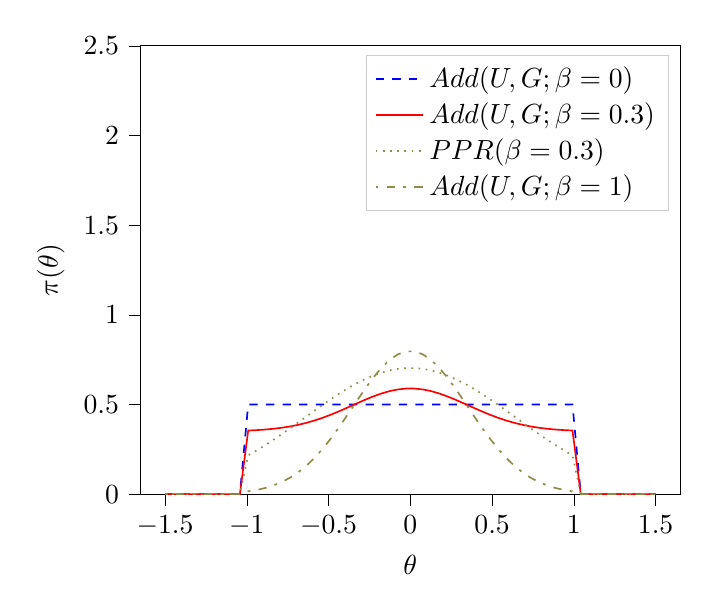
\begin{tikzpicture}

\begin{axis}[
legend cell align={left},
legend style={fill opacity=0.8, draw opacity=1, text opacity=1, draw=white!80!black},
tick align=outside,
tick pos=left,
x grid style={white!69.0196078431373!black},
xlabel={\(\displaystyle \theta\)},
xmin=-1.65, xmax=1.65,
xtick style={color=black},
y grid style={white!69.0196078431373!black},
ylabel={\(\displaystyle \pi(\theta)\)},
ymin=0, ymax=2.5,
ytick style={color=black}
]
\addplot [semithick, blue, dashed]
table {%
-1.5 0
-1.44915254237288 0
-1.39830508474576 0
-1.34745762711864 0
-1.29661016949153 0
-1.24576271186441 0
-1.19491525423729 0
-1.14406779661017 0
-1.09322033898305 0
-1.04237288135593 0
-0.991525423728814 0.5
-0.940677966101695 0.5
-0.889830508474576 0.5
-0.838983050847458 0.5
-0.788135593220339 0.5
-0.73728813559322 0.5
-0.686440677966102 0.5
-0.635593220338983 0.5
-0.584745762711864 0.5
-0.533898305084746 0.5
-0.483050847457627 0.5
-0.432203389830508 0.5
-0.38135593220339 0.5
-0.330508474576271 0.5
-0.279661016949152 0.5
-0.228813559322034 0.5
-0.177966101694915 0.5
-0.127118644067796 0.5
-0.0762711864406778 0.5
-0.0254237288135593 0.5
0.0254237288135595 0.5
0.076271186440678 0.5
0.127118644067797 0.5
0.177966101694915 0.5
0.228813559322034 0.5
0.279661016949153 0.5
0.330508474576271 0.5
0.38135593220339 0.5
0.432203389830509 0.5
0.483050847457627 0.5
0.533898305084746 0.5
0.584745762711865 0.5
0.635593220338983 0.5
0.686440677966102 0.5
0.737288135593221 0.5
0.788135593220339 0.5
0.838983050847458 0.5
0.889830508474577 0.5
0.940677966101695 0.5
0.991525423728814 0.5
1.04237288135593 0
1.09322033898305 0
1.14406779661017 0
1.19491525423729 0
1.24576271186441 0
1.29661016949153 0
1.34745762711864 0
1.39830508474576 0
1.44915254237288 0
1.5 0
};
\addlegendentry{$Add(U, G; \beta=0)$}
\addplot [semithick, red]
table {%
-1.5 0
-1.44915254237288 0
-1.39830508474576 0
-1.34745762711864 0
-1.29661016949153 0
-1.24576271186441 0
-1.19491525423729 0
-1.14406779661017 0
-1.09322033898305 0
-1.04237288135593 0
-0.991525423728814 0.354690318349014
-0.940677966101695 0.356948257984
-0.889830508474576 0.360082465104504
-0.838983050847458 0.364330940676924
-0.788135593220339 0.369952616124693
-0.73728813559322 0.377210854126332
-0.686440677966102 0.386349771016284
-0.635593220338983 0.397563999166328
-0.584745762711864 0.410963827347145
-0.533898305084746 0.426539084688447
-0.483050847457627 0.444126407270881
-0.432203389830508 0.463385332657938
-0.38135593220339 0.483788705911657
-0.330508474576271 0.504631940380111
-0.279661016949152 0.525063713430144
-0.228813559322034 0.54413786330865
-0.177966101694915 0.560882981292239
-0.127118644067796 0.574383024711279
-0.0762711864406778 0.583859836479305
-0.0254237288135593 0.588747297055759
0.0254237288135595 0.588747297055759
0.076271186440678 0.583859836479305
0.127118644067797 0.574383024711279
0.177966101694915 0.560882981292239
0.228813559322034 0.54413786330865
0.279661016949153 0.525063713430144
0.330508474576271 0.504631940380111
0.38135593220339 0.483788705911657
0.432203389830509 0.463385332657938
0.483050847457627 0.444126407270881
0.533898305084746 0.426539084688447
0.584745762711865 0.410963827347145
0.635593220338983 0.397563999166328
0.686440677966102 0.386349771016284
0.737288135593221 0.377210854126332
0.788135593220339 0.369952616124693
0.838983050847458 0.364330940676924
0.889830508474577 0.360082465104504
0.940677966101695 0.356948257984
0.991525423728814 0.354690318349014
1.04237288135593 0
1.09322033898305 0
1.14406779661017 0
1.19491525423729 0
1.24576271186441 0
1.29661016949153 0
1.34745762711864 0
1.39830508474576 0
1.44915254237288 0
1.5 0
};
\addlegendentry{$Add(U, G;\beta=0.3)$}
\addplot [semithick, yellow!50!black, dotted]
table {%
-1.5 0
-1.44915254237288 0
-1.39830508474576 0
-1.34745762711864 0
-1.29661016949153 0
-1.24576271186441 0
-1.19491525423729 0
-1.14406779661017 0
-1.09322033898305 0
-1.04237288135593 0
-0.991525423728814 0.216189593234766
-0.940677966101695 0.243241049554894
-0.889830508474576 0.27198446961261
-0.838983050847458 0.302243171403917
-0.788135593220339 0.333790553940582
-0.73728813559322 0.366350459314597
-0.686440677966102 0.399599183303834
-0.635593220338983 0.433169227869832
-0.584745762711864 0.466654819495022
-0.533898305084746 0.499619139927575
-0.483050847457627 0.531603134276833
-0.432203389830508 0.56213567986932
-0.38135593220339 0.59074482252954
-0.330508474576271 0.616969719742002
-0.279661016949152 0.640372876960198
-0.228813559322034 0.660552228031033
-0.177966101694915 0.677152596268245
-0.127118644067796 0.689876080941671
-0.0762711864406778 0.698490945314958
-0.0254237288135593 0.702838635897227
0.0254237288135595 0.702838635897227
0.076271186440678 0.698490945314958
0.127118644067797 0.689876080941671
0.177966101694915 0.677152596268245
0.228813559322034 0.660552228031033
0.279661016949153 0.640372876960198
0.330508474576271 0.616969719742002
0.38135593220339 0.59074482252954
0.432203389830509 0.56213567986932
0.483050847457627 0.531603134276833
0.533898305084746 0.499619139927575
0.584745762711865 0.466654819495021
0.635593220338983 0.433169227869832
0.686440677966102 0.399599183303834
0.737288135593221 0.366350459314597
0.788135593220339 0.333790553940582
0.838983050847458 0.302243171403917
0.889830508474577 0.27198446961261
0.940677966101695 0.243241049554894
0.991525423728814 0.216189593234766
1.04237288135593 0
1.09322033898305 0
1.14406779661017 0
1.19491525423729 0
1.24576271186441 0
1.29661016949153 0
1.34745762711864 0
1.39830508474576 0
1.44915254237288 0
1.5 0
};
\addlegendentry{$PPR(\beta=0.3)$}
\addplot [semithick, yellow!50!black, dash pattern=on 1pt off 3pt on 3pt off 3pt]
table {%
-1.5 0
-1.44915254237288 0
-1.39830508474576 0
-1.34745762711864 0
-1.29661016949153 0
-1.24576271186441 0
-1.19491525423729 0
-1.14406779661017 0
-1.09322033898305 0
-1.04237288135593 0
-0.991525423728814 0.015634394496712
-0.940677966101695 0.0231608599466659
-0.889830508474576 0.0336082170150122
-0.838983050847458 0.0477698022564135
-0.788135593220339 0.066508720415643
-0.73728813559322 0.0907028470877726
-0.686440677966102 0.121165903387615
-0.635593220338983 0.15854666388776
-0.584745762711864 0.203212757823817
-0.533898305084746 0.255130282294824
-0.483050847457627 0.313754690902936
-0.432203389830508 0.377951108859794
-0.38135593220339 0.445962353038858
-0.330508474576271 0.515439801267037
-0.279661016949152 0.583545711433813
-0.228813559322034 0.647126211028834
-0.177966101694915 0.702943270974129
-0.127118644067796 0.747943415704262
-0.0762711864406778 0.77953278826435
-0.0254237288135593 0.795824323519198
0.0254237288135595 0.795824323519198
0.076271186440678 0.77953278826435
0.127118644067797 0.747943415704262
0.177966101694915 0.702943270974129
0.228813559322034 0.647126211028834
0.279661016949153 0.583545711433812
0.330508474576271 0.515439801267037
0.38135593220339 0.445962353038858
0.432203389830509 0.377951108859794
0.483050847457627 0.313754690902936
0.533898305084746 0.255130282294824
0.584745762711865 0.203212757823817
0.635593220338983 0.15854666388776
0.686440677966102 0.121165903387615
0.737288135593221 0.0907028470877724
0.788135593220339 0.0665087204156429
0.838983050847458 0.0477698022564135
0.889830508474577 0.0336082170150121
0.940677966101695 0.0231608599466659
0.991525423728814 0.015634394496712
1.04237288135593 0
1.09322033898305 0
1.14406779661017 0
1.19491525423729 0
1.24576271186441 0
1.29661016949153 0
1.34745762711864 0
1.39830508474576 0
1.44915254237288 0
1.5 0
};
\addlegendentry{$Add(U, G; \beta=1)$}
\end{axis}

\end{tikzpicture}

  \caption{\label{fig:additive} An additive isometric mixture of a
    Gaussian proposal and a uniform reference. Power-Gaussian added
    for comparison.}
\end{figure}

Isometric mixtures are an attempt to relax some of the limitations
imposed by power posterior repartitioning. Firstly, all proposals in
PPR have to be linked by a power relation.  This class always includes
a uniform prior, but not, for example, a ``wedding cake'' prior
(stepped uniform prior). Additive mixtures permit such
proposals. Moreover, in additive isometric mixtures, any consistent
partitions are compatible provided the set union of their domains
matches $\Psi$.

However, additive mixtures have limited utility: they are slow,
difficult to implement and susceptible to numerical instability more
than any other consistent partitioning\footnote{These claims shall be
  substantiated in a more detailed publication.}.  We can, however do
much better.

\subsubsection{Stochastic superpositional isometric mixtures}

One major problem with additive mixtures lies in the definition of
$\hat{\cal L}$. Instead of having to evaluate only one of the
constituent likelihoods, we are forced to evaluate all of them. Hence,
a lower bound on time complexity:
\begin{equation}
  {\cal T}\{\hat{\cal L}\} = o \left(   \max_{i} {\cal T}\{ {\cal L}_{i}\} \right), \label{eq:hard-cap}
\end{equation}
which is the average case when the likelihoods ${\cal L}_{i}$ are all
related to the same reference (e.g.~$\bar{\cal L}$) with only minor
corrections computed asynchronously to account for different
proposals. If ${\cal L}_{i}$ and ${\cal L}_{j}$ have no common
computations to re-use, the average case time complexity is
\(o\left[{\cal T}({\cal L}_{i}) + {\cal T}({\cal L}_{j})\right]\).


Another issue is that the overall likelihood depends on the prior PDFs
of the constituents. This is problematic since nested sampling
requires specification of the prior via its quantile
\citep{Skilling2006,polychord,multinest}. Function inversion is not
linear with respect to addition, so the quantile of the weighted sum
needs to be evaluated for each type of mixture individually. For a
linear combination of uniform priors, evaluating the quantile can be
performed analytically, but not in case of two Gaussians or a Gaussian
mixed with a uniform. By contrast, the quantile of PPR with an
uncorrelated\footnote{not so for a correlated Gaussian. Nonetheless,
  every correlated covariance matrix can be diagonalised, and included
  in the re-parametrisation. } Gaussian proposal is found in closed
form.

We thus try to avoid mathematical operations that require evaluation
of all of the constituents' priors/likelihoods. An example of such an
operation is deterministic prior branching.  This scheme has the
benefit of trivially determining the quantile of the mixture from the
component quantiles. The probability of branch choice can be tuned
using a parameter, which can be made part $\hat{\bm{\theta}}$
similarly to $\beta$ in PPR. This parametrisation provides the
mechanism needed for \cref{vconv-prop}.

Hence, we purport that a \textbf{\emph{superpositional mixture}}, defined via
the following parametrisation:
\begin{subequations}
\begin{equation}
  \hat{\pi}(\bm{\theta}; \bm{\beta})  =
  \begin{cases}
	\hat{\pi}_{1}(\bm{\theta}) & \text{with probability } \beta_{1},\\
	& \vdots\\
	\hat{\pi}_{n}(\bm{\theta}) & \text{with probability } (1- \sum_{i}^{m}\beta_{i}),
	\end{cases}
\end{equation}
\begin{equation}
  \hat{\cal L}(\bm{\theta}; \bm{\beta})  =
  \begin{cases}
	\hat{\cal L}_{1}(\bm{\theta}) &  \text{with probability } \beta_{1},\\
		    &\vdots\\
	\hat{\cal L}_{m}(\bm{\theta}) & \text{with probability} (1- \sum_{i}^{m}\beta_{i}).
\end{cases}
\end{equation}
is isometric, if and only if
\begin{equation}
  \label{eq:sspr}
  \hat{\pi}(\bm{\theta}; \bm{\beta}) = \hat{\pi}_{i}(\bm{\theta}) \Leftrightarrow \hat{\cal L}(\bm{\theta}; \bm{\beta}) = \hat{\cal L}_{i}(\bm{\theta}; \bm{\beta}), 
\end{equation}
\end{subequations}
that is, the branches are chosen consistently. 

The~\cref{spec-prop} is satisfied, if any of the priors $\hat{\pi}$
represented the posterior. The~\cref{vconv-prop} is satisfied
similarly to PPR: the likelihood is determined by
\(\bm\hat{\theta} \supset \bm{\beta}\), so $\bm{\beta}$s that lead to
higher likelihoods are favoured, ergo configurations representing
${\cal P}$ are preferred.

Superpositional mixtures have multiple advantages when compared with
additive mixtures. Crucially, only one of ${\cal L}_{i}$ is evaluated
each time $\hat{\cal L}$ is evaluated. As a result, ignoring the
overhead of branch choice, the worst-case time complexity is the same
if not better than the best case for additive mixtures, which has vast
implications discussed in \cref{sec:applications}.

The superpositional mixture's branch choice must be external to and
independent from the likelihoods and priors. For example, the prior
quantile of the mixture must branch into either of the component prior
quantiles. As a result, the end user doesn't need to perform any
calculations beyond the proposal quantiles themselves.

There can be many implementations of a superpositional mixture. A
natural first choice would be a quantum computer, where the
$\hat{\pi}$ and $\hat{\cal L}$ are represented by \(m\) level systems
entangled with each other (consistent branching) and a classical
computer (to evaluate ${\cal L}$ and $\pi$). However, we can also
attain an implementation using only computational methods via
stochastic deterministic choice based on $\bm{\theta}$.

The \textbf{\emph{stochastic superpositional (isometric) mixture}} of
consistent partitioning (SSIM) ensures branch consistency by requiring
\begin{equation}
\hat{\pi}(\bm{\theta}; \bm{\beta}) = \hat{\pi}_{F(\bm{\theta};
  \bm{\beta})}(\bm{\theta};\bm{\beta}),
\end{equation}
where
$F: (\bm{\theta}, \bm{\beta}) \mapsto i \in \{1, 2, \ldots, m-1\}$. In
our implementation it is a niche-apportionment random number generator
(sometimes called the broken stick model), seeded with the numerical
\texttt{hash} of the vector $\bm{\theta}$, illustrated in
\cref{fig:mixture}.

Superpositional mixtures are superior in robustness and ease of
implementation. They do, nevertheless, come with one drawback. As a
result of branching, the likelihood $\hat{\cal L}$ visible to the
sampler, is no longer continuous (\cref{fig:mixture-3d}). Thus a
nested sampling implementation that relied on said continuity will
have undefined behaviour. \texttt{PolyChord}'s slice sampling seems
not affected by the discontinuity, but there may be other samplers
that are.
\begin{figure}  
  % This file was created by tikzplotlib v0.9.1.
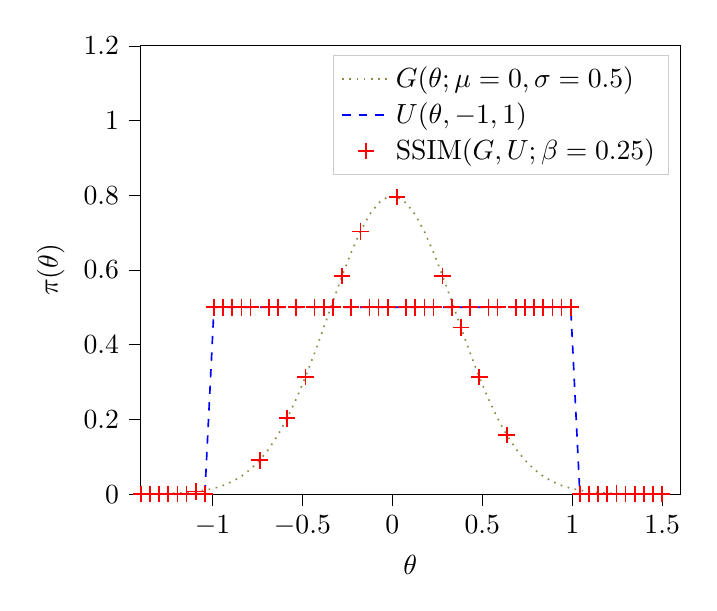
\begin{tikzpicture}

\begin{axis}[
legend cell align={left},
legend style={fill opacity=0.8, draw opacity=1, text opacity=1, draw=white!80!black},
tick align=outside,
tick pos=left,
x grid style={white!69.0196078431373!black},
xlabel={\(\displaystyle \theta\)},
xmin=-1.4, xmax=1.6,
xtick style={color=black},
y grid style={white!69.0196078431373!black},
ylabel={\(\displaystyle \pi(\theta)\)},
ymin=0, ymax=1.2,
ytick style={color=black}
]
\addplot [semithick, yellow!50!black, dotted]
table {%
-1.5 9.8466777332468e-05
-1.44915254237288 0.0001793872435764
-1.39830508474576 0.000320118348094559
-1.34745762711864 0.000559560121531124
-1.29661016949153 0.000958076356441112
-1.24576271186441 0.00160683272401611
-1.19491525423729 0.00263972321036136
-1.14406779661017 0.00424779248787262
-1.09322033898305 0.00669553635076534
-1.04237288135593 0.0103377167883577
-0.991525423728814 0.015634394496712
-0.940677966101695 0.0231608599466659
-0.889830508474576 0.0336082170150122
-0.838983050847458 0.0477698022564135
-0.788135593220339 0.066508720415643
-0.73728813559322 0.0907028470877726
-0.686440677966102 0.121165903387615
-0.635593220338983 0.15854666388776
-0.584745762711864 0.203212757823817
-0.533898305084746 0.255130282294824
-0.483050847457627 0.313754690902936
-0.432203389830508 0.377951108859794
-0.38135593220339 0.445962353038858
-0.330508474576271 0.515439801267037
-0.279661016949152 0.583545711433813
-0.228813559322034 0.647126211028834
-0.177966101694915 0.702943270974129
-0.127118644067796 0.747943415704262
-0.0762711864406778 0.77953278826435
-0.0254237288135593 0.795824323519198
0.0254237288135595 0.795824323519198
0.076271186440678 0.77953278826435
0.127118644067797 0.747943415704262
0.177966101694915 0.702943270974129
0.228813559322034 0.647126211028834
0.279661016949153 0.583545711433812
0.330508474576271 0.515439801267037
0.38135593220339 0.445962353038858
0.432203389830509 0.377951108859794
0.483050847457627 0.313754690902936
0.533898305084746 0.255130282294824
0.584745762711865 0.203212757823817
0.635593220338983 0.15854666388776
0.686440677966102 0.121165903387615
0.737288135593221 0.0907028470877724
0.788135593220339 0.0665087204156429
0.838983050847458 0.0477698022564135
0.889830508474577 0.0336082170150121
0.940677966101695 0.0231608599466659
0.991525423728814 0.015634394496712
1.04237288135593 0.0103377167883577
1.09322033898305 0.00669553635076532
1.14406779661017 0.00424779248787262
1.19491525423729 0.00263972321036135
1.24576271186441 0.0016068327240161
1.29661016949153 0.000958076356441112
1.34745762711864 0.000559560121531121
1.39830508474576 0.000320118348094558
1.44915254237288 0.000179387243576399
1.5 9.8466777332468e-05
};
\addlegendentry{$G(\theta; \mu=0, \sigma=0.5)$}
\addplot [semithick, blue, dashed]
table {%
-1.5 0
-1.44915254237288 0
-1.39830508474576 0
-1.34745762711864 0
-1.29661016949153 0
-1.24576271186441 0
-1.19491525423729 0
-1.14406779661017 0
-1.09322033898305 0
-1.04237288135593 0
-0.991525423728814 0.5
-0.940677966101695 0.5
-0.889830508474576 0.5
-0.838983050847458 0.5
-0.788135593220339 0.5
-0.73728813559322 0.5
-0.686440677966102 0.5
-0.635593220338983 0.5
-0.584745762711864 0.5
-0.533898305084746 0.5
-0.483050847457627 0.5
-0.432203389830508 0.5
-0.38135593220339 0.5
-0.330508474576271 0.5
-0.279661016949152 0.5
-0.228813559322034 0.5
-0.177966101694915 0.5
-0.127118644067796 0.5
-0.0762711864406778 0.5
-0.0254237288135593 0.5
0.0254237288135595 0.5
0.076271186440678 0.5
0.127118644067797 0.5
0.177966101694915 0.5
0.228813559322034 0.5
0.279661016949153 0.5
0.330508474576271 0.5
0.38135593220339 0.5
0.432203389830509 0.5
0.483050847457627 0.5
0.533898305084746 0.5
0.584745762711865 0.5
0.635593220338983 0.5
0.686440677966102 0.5
0.737288135593221 0.5
0.788135593220339 0.5
0.838983050847458 0.5
0.889830508474577 0.5
0.940677966101695 0.5
0.991525423728814 0.5
1.04237288135593 0
1.09322033898305 0
1.14406779661017 0
1.19491525423729 0
1.24576271186441 0
1.29661016949153 0
1.34745762711864 0
1.39830508474576 0
1.44915254237288 0
1.5 0
};
\addlegendentry{$U(\theta, -1, 1)$}
\addplot [semithick, red, mark=+, mark size=3, mark options={solid}, only marks]
table {%
-1.5 0
-1.44915254237288 0
-1.39830508474576 0
-1.34745762711864 0
-1.29661016949153 0
-1.24576271186441 0
-1.19491525423729 0
-1.14406779661017 0
-1.09322033898305 0.00669553635076534
-1.04237288135593 0
-0.991525423728814 0.5
-0.940677966101695 0.5
-0.889830508474576 0.5
-0.838983050847458 0.5
-0.788135593220339 0.5
-0.73728813559322 0.0907028470877726
-0.686440677966102 0.5
-0.635593220338983 0.5
-0.584745762711864 0.203212757823817
-0.533898305084746 0.5
-0.483050847457627 0.313754690902936
-0.432203389830508 0.5
-0.38135593220339 0.5
-0.330508474576271 0.5
-0.279661016949152 0.583545711433813
-0.228813559322034 0.5
-0.177966101694915 0.702943270974129
-0.127118644067796 0.5
-0.0762711864406778 0.5
-0.0254237288135593 0.5
0.0254237288135595 0.795824323519198
0.076271186440678 0.5
0.127118644067797 0.5
0.177966101694915 0.5
0.228813559322034 0.5
0.279661016949153 0.583545711433812
0.330508474576271 0.5
0.38135593220339 0.445962353038858
0.432203389830509 0.5
0.483050847457627 0.313754690902936
0.533898305084746 0.5
0.584745762711865 0.5
0.635593220338983 0.15854666388776
0.686440677966102 0.5
0.737288135593221 0.5
0.788135593220339 0.5
0.838983050847458 0.5
0.889830508474577 0.5
0.940677966101695 0.5
0.991525423728814 0.5
1.04237288135593 0
1.09322033898305 0
1.14406779661017 0
1.19491525423729 0
1.24576271186441 0.0016068327240161
1.29661016949153 0
1.34745762711864 0
1.39830508474576 0
1.44915254237288 0
1.5 0
};
\addlegendentry{SSIM$(G, U; \beta=0.25)$}
\end{axis}

\end{tikzpicture}


  % This file was created by tikzplotlib v0.9.1.
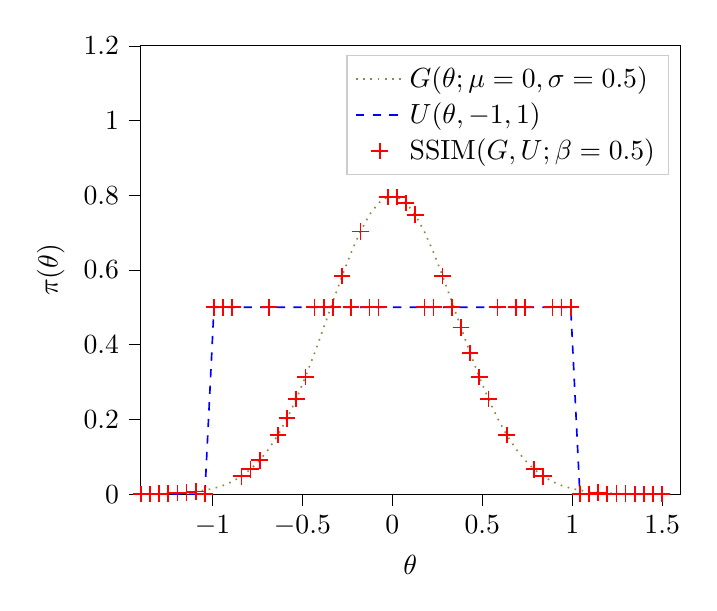
\begin{tikzpicture}

\begin{axis}[
legend cell align={left},
legend style={fill opacity=0.8, draw opacity=1, text opacity=1, draw=white!80!black},
tick align=outside,
tick pos=left,
x grid style={white!69.0196078431373!black},
xlabel={\(\displaystyle \theta\)},
xmin=-1.4, xmax=1.6,
xtick style={color=black},
y grid style={white!69.0196078431373!black},
ylabel={\(\displaystyle \pi(\theta)\)},
ymin=0, ymax=1.2,
ytick style={color=black}
]
\addplot [semithick, yellow!50!black, dotted]
table {%
-1.5 9.8466777332468e-05
-1.44915254237288 0.0001793872435764
-1.39830508474576 0.000320118348094559
-1.34745762711864 0.000559560121531124
-1.29661016949153 0.000958076356441112
-1.24576271186441 0.00160683272401611
-1.19491525423729 0.00263972321036136
-1.14406779661017 0.00424779248787262
-1.09322033898305 0.00669553635076534
-1.04237288135593 0.0103377167883577
-0.991525423728814 0.015634394496712
-0.940677966101695 0.0231608599466659
-0.889830508474576 0.0336082170150122
-0.838983050847458 0.0477698022564135
-0.788135593220339 0.066508720415643
-0.73728813559322 0.0907028470877726
-0.686440677966102 0.121165903387615
-0.635593220338983 0.15854666388776
-0.584745762711864 0.203212757823817
-0.533898305084746 0.255130282294824
-0.483050847457627 0.313754690902936
-0.432203389830508 0.377951108859794
-0.38135593220339 0.445962353038858
-0.330508474576271 0.515439801267037
-0.279661016949152 0.583545711433813
-0.228813559322034 0.647126211028834
-0.177966101694915 0.702943270974129
-0.127118644067796 0.747943415704262
-0.0762711864406778 0.77953278826435
-0.0254237288135593 0.795824323519198
0.0254237288135595 0.795824323519198
0.076271186440678 0.77953278826435
0.127118644067797 0.747943415704262
0.177966101694915 0.702943270974129
0.228813559322034 0.647126211028834
0.279661016949153 0.583545711433812
0.330508474576271 0.515439801267037
0.38135593220339 0.445962353038858
0.432203389830509 0.377951108859794
0.483050847457627 0.313754690902936
0.533898305084746 0.255130282294824
0.584745762711865 0.203212757823817
0.635593220338983 0.15854666388776
0.686440677966102 0.121165903387615
0.737288135593221 0.0907028470877724
0.788135593220339 0.0665087204156429
0.838983050847458 0.0477698022564135
0.889830508474577 0.0336082170150121
0.940677966101695 0.0231608599466659
0.991525423728814 0.015634394496712
1.04237288135593 0.0103377167883577
1.09322033898305 0.00669553635076532
1.14406779661017 0.00424779248787262
1.19491525423729 0.00263972321036135
1.24576271186441 0.0016068327240161
1.29661016949153 0.000958076356441112
1.34745762711864 0.000559560121531121
1.39830508474576 0.000320118348094558
1.44915254237288 0.000179387243576399
1.5 9.8466777332468e-05
};
\addlegendentry{$G(\theta; \mu=0, \sigma=0.5)$}
\addplot [semithick, blue, dashed]
table {%
-1.5 0
-1.44915254237288 0
-1.39830508474576 0
-1.34745762711864 0
-1.29661016949153 0
-1.24576271186441 0
-1.19491525423729 0
-1.14406779661017 0
-1.09322033898305 0
-1.04237288135593 0
-0.991525423728814 0.5
-0.940677966101695 0.5
-0.889830508474576 0.5
-0.838983050847458 0.5
-0.788135593220339 0.5
-0.73728813559322 0.5
-0.686440677966102 0.5
-0.635593220338983 0.5
-0.584745762711864 0.5
-0.533898305084746 0.5
-0.483050847457627 0.5
-0.432203389830508 0.5
-0.38135593220339 0.5
-0.330508474576271 0.5
-0.279661016949152 0.5
-0.228813559322034 0.5
-0.177966101694915 0.5
-0.127118644067796 0.5
-0.0762711864406778 0.5
-0.0254237288135593 0.5
0.0254237288135595 0.5
0.076271186440678 0.5
0.127118644067797 0.5
0.177966101694915 0.5
0.228813559322034 0.5
0.279661016949153 0.5
0.330508474576271 0.5
0.38135593220339 0.5
0.432203389830509 0.5
0.483050847457627 0.5
0.533898305084746 0.5
0.584745762711865 0.5
0.635593220338983 0.5
0.686440677966102 0.5
0.737288135593221 0.5
0.788135593220339 0.5
0.838983050847458 0.5
0.889830508474577 0.5
0.940677966101695 0.5
0.991525423728814 0.5
1.04237288135593 0
1.09322033898305 0
1.14406779661017 0
1.19491525423729 0
1.24576271186441 0
1.29661016949153 0
1.34745762711864 0
1.39830508474576 0
1.44915254237288 0
1.5 0
};
\addlegendentry{$U(\theta, -1, 1)$}
\addplot [semithick, red, mark=+, mark size=3, mark options={solid}, only marks]
table {%
-1.5 9.8466777332468e-05
-1.44915254237288 0.0001793872435764
-1.39830508474576 0
-1.34745762711864 0.000559560121531124
-1.29661016949153 0.000958076356441112
-1.24576271186441 0.00160683272401611
-1.19491525423729 0.00263972321036136
-1.14406779661017 0.00424779248787262
-1.09322033898305 0.00669553635076534
-1.04237288135593 0
-0.991525423728814 0.5
-0.940677966101695 0.5
-0.889830508474576 0.5
-0.838983050847458 0.0477698022564135
-0.788135593220339 0.066508720415643
-0.73728813559322 0.0907028470877726
-0.686440677966102 0.5
-0.635593220338983 0.15854666388776
-0.584745762711864 0.203212757823817
-0.533898305084746 0.255130282294824
-0.483050847457627 0.313754690902936
-0.432203389830508 0.5
-0.38135593220339 0.5
-0.330508474576271 0.5
-0.279661016949152 0.583545711433813
-0.228813559322034 0.5
-0.177966101694915 0.702943270974129
-0.127118644067796 0.5
-0.0762711864406778 0.5
-0.0254237288135593 0.795824323519198
0.0254237288135595 0.795824323519198
0.076271186440678 0.77953278826435
0.127118644067797 0.747943415704262
0.177966101694915 0.5
0.228813559322034 0.5
0.279661016949153 0.583545711433812
0.330508474576271 0.5
0.38135593220339 0.445962353038858
0.432203389830509 0.377951108859794
0.483050847457627 0.313754690902936
0.533898305084746 0.255130282294824
0.584745762711865 0.5
0.635593220338983 0.15854666388776
0.686440677966102 0.5
0.737288135593221 0.5
0.788135593220339 0.0665087204156429
0.838983050847458 0.0477698022564135
0.889830508474577 0.5
0.940677966101695 0.5
0.991525423728814 0.5
1.04237288135593 0
1.09322033898305 0
1.14406779661017 0.00424779248787262
1.19491525423729 0
1.24576271186441 0.0016068327240161
1.29661016949153 0.000958076356441112
1.34745762711864 0
1.39830508474576 0.000320118348094558
1.44915254237288 0
1.5 9.8466777332468e-05
};
\addlegendentry{SSIM$(G, U; \beta=0.5)$}
\end{axis}

\end{tikzpicture}


  % This file was created by tikzplotlib v0.9.1.
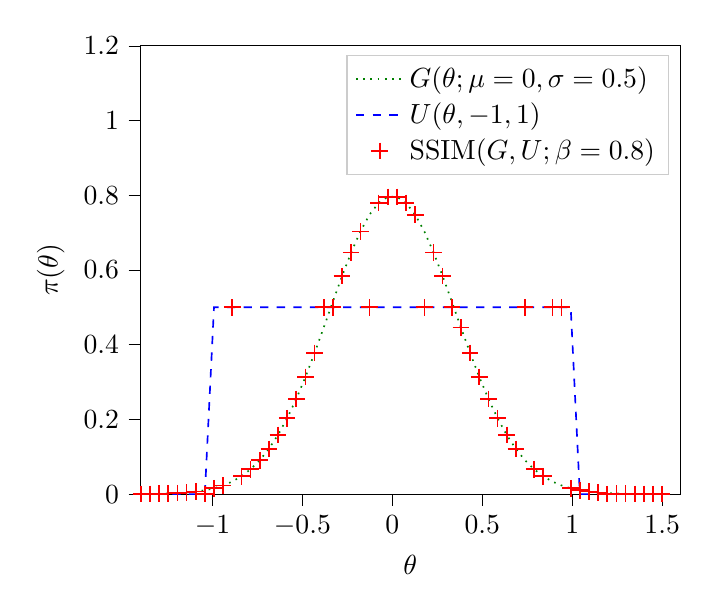
\begin{tikzpicture}

\begin{axis}[
legend cell align={left},
legend style={fill opacity=0.8, draw opacity=1, text opacity=1, draw=white!80!black},
tick align=outside,
tick pos=left,
x grid style={white!69.0196078431373!black},
xlabel={\(\displaystyle \theta\)},
xmin=-1.4, xmax=1.6,
xtick style={color=black},
y grid style={white!69.0196078431373!black},
ylabel={\(\displaystyle \pi(\theta)\)},
ymin=0, ymax=1.2,
ytick style={color=black}
]
\addplot [semithick, green!50!black, dotted]
table {%
-1.5 9.8466777332468e-05
-1.44915254237288 0.0001793872435764
-1.39830508474576 0.000320118348094559
-1.34745762711864 0.000559560121531124
-1.29661016949153 0.000958076356441112
-1.24576271186441 0.00160683272401611
-1.19491525423729 0.00263972321036136
-1.14406779661017 0.00424779248787262
-1.09322033898305 0.00669553635076534
-1.04237288135593 0.0103377167883577
-0.991525423728814 0.015634394496712
-0.940677966101695 0.0231608599466659
-0.889830508474576 0.0336082170150122
-0.838983050847458 0.0477698022564135
-0.788135593220339 0.066508720415643
-0.73728813559322 0.0907028470877726
-0.686440677966102 0.121165903387615
-0.635593220338983 0.15854666388776
-0.584745762711864 0.203212757823817
-0.533898305084746 0.255130282294824
-0.483050847457627 0.313754690902936
-0.432203389830508 0.377951108859794
-0.38135593220339 0.445962353038858
-0.330508474576271 0.515439801267037
-0.279661016949152 0.583545711433813
-0.228813559322034 0.647126211028834
-0.177966101694915 0.702943270974129
-0.127118644067796 0.747943415704262
-0.0762711864406778 0.77953278826435
-0.0254237288135593 0.795824323519198
0.0254237288135595 0.795824323519198
0.076271186440678 0.77953278826435
0.127118644067797 0.747943415704262
0.177966101694915 0.702943270974129
0.228813559322034 0.647126211028834
0.279661016949153 0.583545711433812
0.330508474576271 0.515439801267037
0.38135593220339 0.445962353038858
0.432203389830509 0.377951108859794
0.483050847457627 0.313754690902936
0.533898305084746 0.255130282294824
0.584745762711865 0.203212757823817
0.635593220338983 0.15854666388776
0.686440677966102 0.121165903387615
0.737288135593221 0.0907028470877724
0.788135593220339 0.0665087204156429
0.838983050847458 0.0477698022564135
0.889830508474577 0.0336082170150121
0.940677966101695 0.0231608599466659
0.991525423728814 0.015634394496712
1.04237288135593 0.0103377167883577
1.09322033898305 0.00669553635076532
1.14406779661017 0.00424779248787262
1.19491525423729 0.00263972321036135
1.24576271186441 0.0016068327240161
1.29661016949153 0.000958076356441112
1.34745762711864 0.000559560121531121
1.39830508474576 0.000320118348094558
1.44915254237288 0.000179387243576399
1.5 9.8466777332468e-05
};
\addlegendentry{$G(\theta; \mu=0, \sigma=0.5)$}
\addplot [semithick, blue, dashed]
table {%
-1.5 0
-1.44915254237288 0
-1.39830508474576 0
-1.34745762711864 0
-1.29661016949153 0
-1.24576271186441 0
-1.19491525423729 0
-1.14406779661017 0
-1.09322033898305 0
-1.04237288135593 0
-0.991525423728814 0.5
-0.940677966101695 0.5
-0.889830508474576 0.5
-0.838983050847458 0.5
-0.788135593220339 0.5
-0.73728813559322 0.5
-0.686440677966102 0.5
-0.635593220338983 0.5
-0.584745762711864 0.5
-0.533898305084746 0.5
-0.483050847457627 0.5
-0.432203389830508 0.5
-0.38135593220339 0.5
-0.330508474576271 0.5
-0.279661016949152 0.5
-0.228813559322034 0.5
-0.177966101694915 0.5
-0.127118644067796 0.5
-0.0762711864406778 0.5
-0.0254237288135593 0.5
0.0254237288135595 0.5
0.076271186440678 0.5
0.127118644067797 0.5
0.177966101694915 0.5
0.228813559322034 0.5
0.279661016949153 0.5
0.330508474576271 0.5
0.38135593220339 0.5
0.432203389830509 0.5
0.483050847457627 0.5
0.533898305084746 0.5
0.584745762711865 0.5
0.635593220338983 0.5
0.686440677966102 0.5
0.737288135593221 0.5
0.788135593220339 0.5
0.838983050847458 0.5
0.889830508474577 0.5
0.940677966101695 0.5
0.991525423728814 0.5
1.04237288135593 0
1.09322033898305 0
1.14406779661017 0
1.19491525423729 0
1.24576271186441 0
1.29661016949153 0
1.34745762711864 0
1.39830508474576 0
1.44915254237288 0
1.5 0
};
\addlegendentry{$U(\theta, -1, 1)$}
\addplot [semithick, red, mark=+, mark size=3, mark options={solid}, only marks]
table {%
-1.5 9.8466777332468e-05
-1.44915254237288 0.0001793872435764
-1.39830508474576 0
-1.34745762711864 0.000559560121531124
-1.29661016949153 0.000958076356441112
-1.24576271186441 0.00160683272401611
-1.19491525423729 0.00263972321036136
-1.14406779661017 0.00424779248787262
-1.09322033898305 0.00669553635076534
-1.04237288135593 0
-0.991525423728814 0.015634394496712
-0.940677966101695 0.0231608599466659
-0.889830508474576 0.5
-0.838983050847458 0.0477698022564135
-0.788135593220339 0.066508720415643
-0.73728813559322 0.0907028470877726
-0.686440677966102 0.121165903387615
-0.635593220338983 0.15854666388776
-0.584745762711864 0.203212757823817
-0.533898305084746 0.255130282294824
-0.483050847457627 0.313754690902936
-0.432203389830508 0.377951108859794
-0.38135593220339 0.5
-0.330508474576271 0.5
-0.279661016949152 0.583545711433813
-0.228813559322034 0.647126211028834
-0.177966101694915 0.702943270974129
-0.127118644067796 0.5
-0.0762711864406778 0.77953278826435
-0.0254237288135593 0.795824323519198
0.0254237288135595 0.795824323519198
0.076271186440678 0.77953278826435
0.127118644067797 0.747943415704262
0.177966101694915 0.5
0.228813559322034 0.647126211028834
0.279661016949153 0.583545711433812
0.330508474576271 0.5
0.38135593220339 0.445962353038858
0.432203389830509 0.377951108859794
0.483050847457627 0.313754690902936
0.533898305084746 0.255130282294824
0.584745762711865 0.203212757823817
0.635593220338983 0.15854666388776
0.686440677966102 0.121165903387615
0.737288135593221 0.5
0.788135593220339 0.0665087204156429
0.838983050847458 0.0477698022564135
0.889830508474577 0.5
0.940677966101695 0.5
0.991525423728814 0.015634394496712
1.04237288135593 0.0103377167883577
1.09322033898305 0.00669553635076532
1.14406779661017 0.00424779248787262
1.19491525423729 0
1.24576271186441 0.0016068327240161
1.29661016949153 0.000958076356441112
1.34745762711864 0.000559560121531121
1.39830508474576 0.000320118348094558
1.44915254237288 0.000179387243576399
1.5 9.8466777332468e-05
};
\addlegendentry{SSIM$(G, U; \beta=0.8)$}
\end{axis}

\end{tikzpicture}

  \caption{An example of mixture repartitioning. The mixture is not
    normalised to emphasise the coincidence of values with both the
    uniform distribution and a Gaussian. $\beta$ controls the
    probability of belonging to the Gaussian in the stochastic
    mixture.  Additionally, the resolution is deliberately reduced, to
    contrast behaviour of all three at the truncation
    boundary. \label{fig:mixture}}
\end{figure}

\begin{figure}
  \centering
  \includegraphics[width=0.99\columnwidth]{./illustrations/SSIM_3d.pdf}
  \caption{An illustration of SSIM in two dimensions. Colour represents the value of $\pi(\bm{\theta})$. As a result of nested sampling, nucleation of the representative phase is dynamically favoured.}
  \label{fig:mixture-3d}
\end{figure}

\subsection{On notation and mental models}

It is opportune time to discuss a subtlety that we have previously
neglected. \cite{chen-ferroz-hobson} originally named the technique
automatic posterior repartitioning, which evokes a clear mental
model. Assuming that the original definitions of \( \pi \) and
\(\mathcal{L}\) were a partitioning of only the posterior, a new value
of \(\beta\) produces a new partitioning, thus it re-partitions the
posterior.  The extra parameter is a time-like object, with a clear
direction of evolution, in that any change to its value causes a
re-partitioning of the model.

While this mental model had served well for the purposes of solving
the unrepresentative prior problem, it is severely limiting to the
effect of introducing proposals.

The first ineptitude of the mental model is that the expression
``re-partitioning'' implies the mutability of the posterior. It is not
mutable. In fact, the posterior that we obtained via re-partitioning
has a strict functional dependence on the parameter, which is strictly
a different function. Meaningful information is lost when we project
the repartitioned result to the original prior space, albeit only a
Bayesian would regard it as such.

A second deeper problem is that the notation inherently puts impetus
on the posterior. In reality automatic posterior repartitioning is a
necessary, but insufficient condition for consistent partitioning. As
long as no coordinate transformation is performed, the difference is
negligible. However, for more complicated cases, e.g.~re-sizeable
prior space schemes, the posterior repartitioning is
under-determined. A naive extension doesn't and indeed can't produce
the expected result, if one considers an extension similar to
\begin{equation}
  \label{eq:naive-extension}
\pi(\theta) \mathcal{L}(\theta) = \hat{\pi}(\theta) \mathcal{\hat{L}}(\theta) 
\end{equation}
one shall obtain nonsense. One can prove (by considering a reference
prior space from which all prior spaces of the same dimensionality
derive via coordinate transformation), that the correct expression is
actually one that preserves the evidence differential element.

What we propose is a much more general world-view and a more accurate
and expressive model. A consistent partitioning involves specifying a
hyperspace that includes the original prior space. The partitioning
into $\pi$ and $\mathcal{L}$ is done once only, when the Bayesian
inference problem is set up. The original posterior is a function in
the original prior (sub)space. The posterior we obtain as a result, is
the original in some projections, the evidence to which it corresponds
is also the same as the original.

One might object that this is not a good model for the superpositional
mixture, as the dynamical analogy would be much more appropriate, as
the parameters really only control the partitioning. This point is
partially valid. I would advocate seeing superpositions as an
extension into a hilbert space of vectors that are themselves
spaces. Not easy to imagine, but to someone fluent in Quantum theory,
not a challenge. A better analogy would be to imagine the spaces for
each individual prior side by side, and have a few parameters that
control the relative ``heights'' of these spaces, or activation energy
for diffusion. This is a middle-ground that retains the generality of
treating the entire problem in a hyperspace, but also has a dynamical
analogy.

Arguments can be made either way, but an important consideration is to
have a model that gives accurate predictions first, and is easy to
imagine second.

\section{Measurements and methodology}
Our measurements have to ascertain three key points. First we must
prove that the consistent partitions obtain sensible estimates of
${\cal P}$ and ${\cal Z}$ and document the circumstances when they
don't. We shall then need to measure the performance uplift that can
be attained while preserving the accuracy and precision of the
sampling. Lastly, we shall test our machinery when applied to a
real-world example: Cosmological parameter estimation.

For performance, we shall adopt the weighted accounting approach
\citep{Cormen} for measuring time complexity in units of
\({\cal N}\{{\cal L}\}\), and reducing all quantities to their
long-run averages. Consequently, all of the partitions' overheads
associated with internal implementation details are ignored. This is
to ensure fairness in comparing power repartitioning to a stochastic
mixture\footnote{SSIM has far less overhead}.

We shall use Kullback-Leibler divergence in two contexts. First,
${\cal D}\{\pi, {\cal P}\}$ --- a measure of information obtained from
the dataset ignoring the prior, is used to gauge performance (as seen
in \Cref{fig:kl-scaling}).

We also need a method of comparing posteriors to determine their
accuracy. The Second divergence
${\cal D}\{ {\cal P}, \bar{\cal P} \}$, quantifies the correctness of
the obtained posterior, where $\bar{\cal P}$ is the posterior obtained
using a $\bar{\pi}(\bm{\theta}) = \text{Const}$. In conjunction with
${\cal Z}$, these form our correctness criteria.

From \cref{eq:bayes}, errors in ${\cal P}$ are necessarily linked to
errors in estimating ${\cal Z}$, and is the pivotal reason why nested
sampling is sensitive to partitioning in the first instance. Moreover,
the character of error in ${\cal Z}$ indicates the type of error in
${\cal P}$. A greater-than-expected evidence ${\cal Z}$ indicates
inconsistent partitioning, where the likelihood was not re-scaled to
accommodate a more informative prior. A less-than-expected ${\cal Z}$
is a sign that the regions of high ${\cal L}$ were not probed
sufficiently, often accompanied by prior imprinting (PPR in
\cref{fig:convergence}).

\begin{table}
  \centering
  
  \caption{Typical values of posterior-to-reference-posterior
    Kullback-Leibler divergence ${\cal D}\{{\cal P}, \bar{\cal P}\}$
    for the runs shown in \cref{fig:hist}. The inconsistent
    re-sizeable uniform had not been given an improper normalisation
    of $\hat{\cal L} = {\cal L}$. It is of type \textbf{\emph{Re-sizeable
        uniform}}.}
  \begin{tabular}{lrr}
    \textbf{Scheme} & ${\cal D}\{ {\cal P}, \bar{\cal P}\}$ & ${\cal Z}$\\
    \hline
    Uniform & 0.018 & \(-62.70 \pm 0.30\)\\
    Analytical & 0.000 & \(-62.72 \pm 0.00\) \\
    $R$ & 0.724 & \(-54.8 \pm 0.90\)\\
    $PPR$ & 0.011 & \(-62.73 \pm 0.01\)\\
    $SSIM(U, G)$ & 0.007 & \(-62.72 \pm 0.01\)\\
    $SSIM(U, G, R)$ & 0.696 & \(-57.70 \pm 0.30\)\\
  \end{tabular}
  \label{tab:hist}
\end{table}


\begin{figure}
  % This file was created by tikzplotlib v0.9.1.
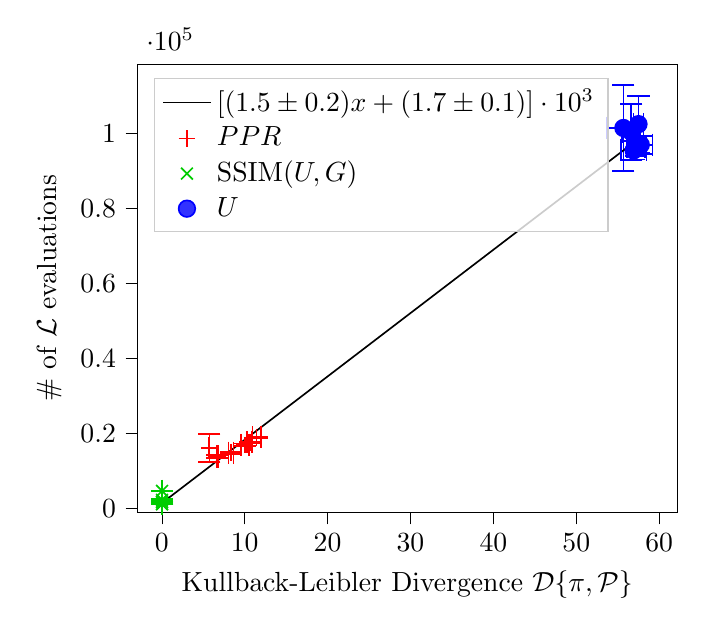
\begin{tikzpicture}

\definecolor{color0}{rgb}{1,0.0,0.0}
\definecolor{color1}{rgb}{0,0.8,0.0}
\definecolor{color2}{rgb}{0.0,0.0,1}
\definecolor{color3}{rgb}{0.0,0.0,0.0}

\begin{axis}[
legend cell align={left},
legend style={fill opacity=0.8, draw opacity=1, text opacity=1, at={(0.03,0.97)}, anchor=north west, draw=white!80!black},
tick align=outside,
tick pos=left,
x grid style={white!69.0196078431373!black},
xlabel={Kullback-Leibler Divergence \(\displaystyle {\cal D} \{\pi, {\cal P}\}\)},
xmin=-2.93567696145677, xmax=62.1613818701095,
xtick style={color=black},
y grid style={white!69.0196078431373!black},
ylabel={\# of \({\cal L}\) evaluations},
ymin=-1000.00, ymax=118545.85,
ytick style={color=black}
% ymode=log
]
\path [draw=color0, semithick]
(axis cs:5.71795365099151,16157.5)
--(axis cs:5.77133948534581,16157.5);

\path [draw=color0, semithick]
(axis cs:6.6768824419002,13953)
--(axis cs:6.77321107556694,13953);

\path [draw=color0, semithick]
(axis cs:8.02877279045042,14940.5)
--(axis cs:8.63543918622054,14940.5);

\path [draw=color0, semithick]
(axis cs:9.52185212376919,17043)
--(axis cs:10.4908349952443,17043);

\path [draw=color0, semithick]
(axis cs:10.3029683750536,17720.5)
--(axis cs:10.9155451202318,17720.5);

\path [draw=color0, semithick]
(axis cs:10.954510866509,19064.5)
--(axis cs:11.9335782130671,19064.5);

\path [draw=color0, semithick]
(axis cs:5.74464656816866,12446)
--(axis cs:5.74464656816866,19869);

\path [draw=color0, semithick]
(axis cs:6.72504675873357,13488)
--(axis cs:6.72504675873357,14418);

\path [draw=color0, semithick]
(axis cs:8.33210598833548,14689)
--(axis cs:8.33210598833548,15192);

\path [draw=color0, semithick]
(axis cs:10.0063435595067,16676)
--(axis cs:10.0063435595067,17410);

\path [draw=color0, semithick]
(axis cs:10.6092567476427,17618)
--(axis cs:10.6092567476427,17823);

\path [draw=color0, semithick]
(axis cs:11.4440445397881,18822)
--(axis cs:11.4440445397881,19307);

\path [draw=color1, semithick]
(axis cs:0.0271909650803472,2382.5)
--(axis cs:0.030089733601838,2382.5);

\path [draw=color1, semithick]
(axis cs:0.029683008672791,1207.5)
--(axis cs:0.0308036500189849,1207.5);

\path [draw=color1, semithick]
(axis cs:0.0282101242046804,1738.5)
--(axis cs:0.0298855157628486,1738.5);

\path [draw=color1, semithick]
(axis cs:0.0278177027329167,4757)
--(axis cs:0.0348526563256524,4757);

\path [draw=color1, semithick]
(axis cs:0.0232802581598788,1829.5)
--(axis cs:0.0301604324600733,1829.5);

\path [draw=color1, semithick]
(axis cs:0.0304771056975755,1224)
--(axis cs:0.0323746358923458,1224);

\path [draw=color1, semithick]
(axis cs:0.0286403493410926,2120)
--(axis cs:0.0286403493410926,2645);

\path [draw=color1, semithick]
(axis cs:0.0302433293458879,1163)
--(axis cs:0.0302433293458879,1252);

\path [draw=color1, semithick]
(axis cs:0.0290478199837645,1565)
--(axis cs:0.0290478199837645,1912);

\path [draw=color1, semithick]
(axis cs:0.0313351795292845,4698)
--(axis cs:0.0313351795292845,4816);

\path [draw=color1, semithick]
(axis cs:0.026720345309976,1740)
--(axis cs:0.026720345309976,1919);

\path [draw=color1, semithick]
(axis cs:0.0314258707949607,1138)
--(axis cs:0.0314258707949607,1310);

\path [draw=color2, semithick]
(axis cs:53.6407046096139,101541)
--(axis cs:57.7293889288474,101541);

\path [draw=color2, semithick]
(axis cs:56.1280894679801,96497)
--(axis cs:58.3022565457241,96497);

\path [draw=color2, semithick]
(axis cs:55.3633380690649,95565)
--(axis cs:58.47445725549,95565);

\path [draw=color2, semithick]
(axis cs:55.5223746731559,100523.5)
--(axis cs:57.7271641567295,100523.5);

\path [draw=color2, semithick]
(axis cs:56.8924880373743,102562.5)
--(axis cs:58.1261131182599,102562.5);

\path [draw=color2, semithick]
(axis cs:56.3603430284318,97066.5)
--(axis cs:59.2024246504929,97066.5);

\path [draw=color2, semithick]
(axis cs:55.6850467692306,90127)
--(axis cs:55.6850467692306,112955);

\path [draw=color2, semithick]
(axis cs:57.2151730068521,94020)
--(axis cs:57.2151730068521,98974);

\path [draw=color2, semithick]
(axis cs:56.9188976622774,93149)
--(axis cs:56.9188976622774,97981);

\path [draw=color2, semithick]
(axis cs:56.6247694149427,93079)
--(axis cs:56.6247694149427,107968);

\path [draw=color2, semithick]
(axis cs:57.5093005778171,94974)
--(axis cs:57.5093005778171,110151);

\path [draw=color2, semithick]
(axis cs:57.7813838394624,94657)
--(axis cs:57.7813838394624,99476);

\addplot [semithick, color0, mark=|, mark size=4, mark options={solid}, only marks, forget plot]
table {%
5.71795365099151 16157.5
6.6768824419002 13953
8.02877279045042 14940.5
9.52185212376919 17043
10.3029683750536 17720.5
10.954510866509 19064.5
};
\addplot [semithick, color0, mark=|, mark size=4, mark options={solid}, only marks, forget plot]
table {%
5.77133948534581 16157.5
6.77321107556694 13953
8.63543918622054 14940.5
10.4908349952443 17043
10.9155451202318 17720.5
11.9335782130671 19064.5
};
\addplot [semithick, color0, mark=-, mark size=4, mark options={solid}, only marks, forget plot]
table {%
5.74464656816866 12446
6.72504675873357 13488
8.33210598833548 14689
10.0063435595067 16676
10.6092567476427 17618
11.4440445397881 18822
};
\addplot [semithick, color0, mark=-, mark size=4, mark options={solid}, only marks, forget plot]
table {%
5.74464656816866 19869
6.72504675873357 14418
8.33210598833548 15192
10.0063435595067 17410
10.6092567476427 17823
11.4440445397881 19307
};
\addplot [semithick, color1, mark=|, mark size=4, mark options={solid}, only marks, forget plot]
table {%
0.0271909650803472 2382.5
0.029683008672791 1207.5
0.0282101242046804 1738.5
0.0278177027329167 4757
0.0232802581598788 1829.5
0.0304771056975755 1224
};
\addplot [semithick, color1, mark=|, mark size=4, mark options={solid}, only marks, forget plot]
table {%
0.030089733601838 2382.5
0.0308036500189849 1207.5
0.0298855157628486 1738.5
0.0348526563256524 4757
0.0301604324600733 1829.5
0.0323746358923458 1224
};
\addplot [semithick, color1, mark=-, mark size=4, mark options={solid}, only marks, forget plot]
table {%
0.0286403493410926 2120
0.0302433293458879 1163
0.0290478199837645 1565
0.0313351795292845 4698
0.026720345309976 1740
0.0314258707949607 1138
};
\addplot [semithick, color1, mark=-, mark size=4, mark options={solid}, only marks, forget plot]
table {%
0.0286403493410926 2645
0.0302433293458879 1252
0.0290478199837645 1912
0.0313351795292845 4816
0.026720345309976 1919
0.0314258707949607 1310
};
\addplot [semithick, color2, mark=|, mark size=4, mark options={solid}, only marks, forget plot]
table {%
53.6407046096139 101541
56.1280894679801 96497
55.3633380690649 95565
55.5223746731559 100523.5
56.8924880373743 102562.5
56.3603430284318 97066.5
};
\addplot [semithick, color2, mark=|, mark size=4, mark options={solid}, only marks, forget plot]
table {%
57.7293889288474 101541
58.3022565457241 96497
58.47445725549 95565
57.7271641567295 100523.5
58.1261131182599 102562.5
59.2024246504929 97066.5
};
\addplot [semithick, color2, mark=-, mark size=4, mark options={solid}, only marks, forget plot]
table {%
55.6850467692306 90127
57.2151730068521 94020
56.9188976622774 93149
56.6247694149427 93079
57.5093005778171 94974
57.7813838394624 94657
};
\addplot [semithick, color2, mark=-, mark size=4, mark options={solid}, only marks, forget plot]
table {%
55.6850467692306 112955
57.2151730068521 98974
56.9188976622774 97981
56.6247694149427 107968
57.5093005778171 110151
57.7813838394624 99476
};
\addplot [semithick, color3]
table {%
0.026720345309976 1539.88164299791
0.610100784644849 2525.39064984014
1.19348122397972 3510.89965668237
1.77686166331459 4496.4086635246
2.36024210264947 5481.91767036683
2.94362254198434 6467.42667720906
3.52700298131921 7452.93568405129
4.11038342065408 8438.44469089352
4.69376385998896 9423.95369773575
5.27714429932383 10409.462704578
5.8605247386587 11394.9717114202
6.44390517799357 12380.4807182624
7.02728561732845 13365.9897251047
7.61066605666332 14351.4987319469
8.19404649599819 15337.0077387891
8.77742693533306 16322.5167456314
9.36080737466794 17308.0257524736
9.94418781400281 18293.5347593158
10.5275682533377 19279.043766158
11.1109486926726 20264.5527730003
11.6943291320074 21250.0617798425
12.2777095713423 22235.5707866847
12.8610900106772 23221.079793527
13.444470450012 24206.5888003692
14.0278508893469 25192.0978072114
14.6112313286818 26177.6068140537
15.1946117680167 27163.1158208959
15.7779922073515 28148.6248277381
16.3613726466864 29134.1338345803
16.9447530860213 30119.6428414226
17.5281335253562 31105.1518482648
18.111513964691 32090.660855107
18.6948944040259 33076.1698619493
19.2782748433608 34061.6788687915
19.8616552826956 35047.1878756337
20.4450357220305 36032.6968824759
21.0284161613654 37018.2058893182
21.6117966007003 38003.7148961604
22.1951770400351 38989.2239030026
22.77855747937 39974.7329098449
23.3619379187049 40960.2419166871
23.9453183580397 41945.7509235293
24.5286987973746 42931.2599303716
25.1120792367095 43916.7689372138
25.6954596760444 44902.277944056
26.2788401153792 45887.7869508982
26.8622205547141 46873.2959577405
27.445600994049 47858.8049645827
28.0289814333839 48844.3139714249
28.6123618727187 49829.8229782672
29.1957423120536 50815.3319851094
29.7791227513885 51800.8409919516
30.3625031907233 52786.3499987938
30.9458836300582 53771.8590056361
31.5292640693931 54757.3680124783
32.112644508728 55742.8770193205
32.6960249480628 56728.3860261628
33.2794053873977 57713.895033005
33.8627858267326 58699.4040398472
34.4461662660675 59684.9130466895
35.0295467054023 60670.4220535317
35.6129271447372 61655.9310603739
36.1963075840721 62641.4400672161
36.7796880234069 63626.9490740584
37.3630684627418 64612.4580809006
37.9464489020767 65597.9670877428
38.5298293414116 66583.4760945851
39.1132097807464 67568.9851014273
39.6965902200813 68554.4941082695
40.2799706594162 69540.0031151118
40.863351098751 70525.512121954
41.4467315380859 71511.0211287962
42.0301119774208 72496.5301356384
42.6134924167557 73482.0391424807
43.1968728560905 74467.5481493229
43.7802532954254 75453.0571561651
44.3636337347603 76438.5661630074
44.9470141740952 77424.0751698496
45.53039461343 78409.5841766918
46.1137750527649 79395.093183534
46.6971554920998 80380.6021903763
47.2805359314346 81366.1111972185
47.8639163707695 82351.6202040607
48.4472968101044 83337.129210903
49.0306772494393 84322.6382177452
49.6140576887741 85308.1472245874
50.197438128109 86293.6562314297
50.7808185674439 87279.1652382719
51.3641990067788 88264.6742451141
51.9475794461136 89250.1832519564
52.5309598854485 90235.6922587986
53.1143403247834 91221.2012656408
53.6977207641182 92206.710272483
54.2811012034531 93192.2192793253
54.864481642788 94177.7282861675
55.4478620821229 95163.2372930097
56.0312425214577 96148.746299852
56.6146229607926 97134.2553066942
57.1980034001275 98119.7643135364
57.7813838394624 99105.2733203786
};
\addlegendentry{\(\left[(1.5 \pm 0.2)x + (1.7 \pm 0.1)\right]\cdot  10^3 \)}
\addplot [semithick, color0, mark=+, mark size=3, mark options={solid}, only marks]
table {%
5.74464656816866 16157.5
6.72504675873357 13953
8.33210598833548 14940.5
10.0063435595067 17043
10.6092567476427 17720.5
11.4440445397881 19064.5
};
\addlegendentry{$PPR$}
\addplot [semithick, color1, mark=x, mark size=3, mark options={solid}, only marks]
table {%
0.0286403493410926 2382.5
0.0302433293458879 1207.5
0.0290478199837645 1738.5
0.0313351795292845 4757
0.026720345309976 1829.5
0.0314258707949607 1224
};
\addlegendentry{SSIM$(U,G)$}
\addplot [semithick, color2, mark=*, mark size=3, mark options={solid}, only marks]
table {%
55.6850467692306 101541
57.2151730068521 96497
56.9188976622774 95565
56.6247694149427 100523.5
57.5093005778171 102562.5
57.7813838394624 97066.5
};
\addlegendentry{$U$}
\end{axis}

\end{tikzpicture}

  \caption{Scaling of number of likelihood calls with Kullback-Leibler
    divergence \({\cal D}\{ \pi, {\cal P}\}\) With co-linear offsets
    varying from $10\bm{\mu}$ to $300\bm{\mu}$. The best fit line is
    \(\left[(1.5 \pm 0.2) {\cal D} + (1.7 \pm 0.1)\right]\cdot 10^3 \)
    with determination coefficient \(R^{2} = 0.85\) which indicates
    that \({\cal D}\) is a reliable performance indicator for
    \texttt{PolyChord}.\label{fig:kl-scaling}}
\end{figure}


\begin{figure}
% This file was created by tikzplotlib v0.9.1.
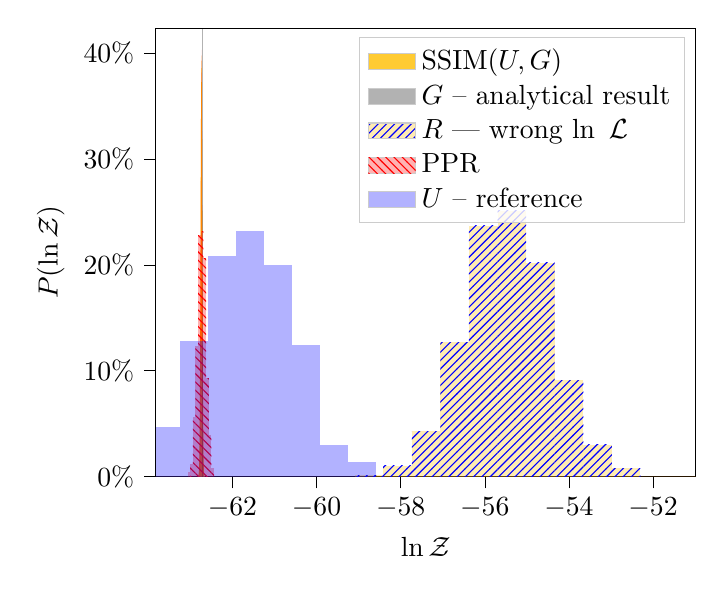
\begin{tikzpicture}

\definecolor{color2}{rgb}{0.0,0.0,1}
\definecolor{color1}{rgb}{1,0.00,0.00}
\definecolor{colorblack}{rgb}{0, 0, 0}
\definecolor{color0}{rgb}{1.0,0.75,0.0}

\begin{axis}[
legend cell align={left},
legend style={fill opacity=0.8, draw opacity=1, text opacity=1, anchor=north east, draw=white!80!black},
tick align=outside,
tick pos=left,
x grid style={white!69.0196078431373!black},
xlabel={\(\ln {\cal Z}\)},
xmin=-63.8198069562379, xmax=-50.9892026507015,
xtick style={color=black},
yticklabel={\pgfmathparse{\tick/10}\pgfmathprintnumber{\pgfmathresult}\%},
y grid style={white!69.0196078431373!black},
ylabel={\(P(\ln {\cal Z})\)},
ymin=0, ymax=423.473092744885,
ytick style={color=black}
]
\path [fill=color0]
(axis cs:-63.8198069562379,0)
--(axis cs:-63.8198069562379,0)
--(axis cs:-63.8069635084846,0)
--(axis cs:-63.7941200607313,0)
--(axis cs:-63.7812766129781,0)
--(axis cs:-63.7684331652248,0)
--(axis cs:-63.7555897174715,0)
--(axis cs:-63.7427462697182,0)
--(axis cs:-63.7299028219649,0)
--(axis cs:-63.7170593742116,0)
--(axis cs:-63.7042159264583,0)
--(axis cs:-63.691372478705,0)
--(axis cs:-63.6785290309517,0)
--(axis cs:-63.6656855831984,0)
--(axis cs:-63.6528421354452,0)
--(axis cs:-63.6399986876919,0)
--(axis cs:-63.6271552399386,0)
--(axis cs:-63.6143117921853,0)
--(axis cs:-63.601468344432,0)
--(axis cs:-63.5886248966787,0)
--(axis cs:-63.5757814489254,0)
--(axis cs:-63.5629380011721,0)
--(axis cs:-63.5500945534188,0)
--(axis cs:-63.5372511056656,0)
--(axis cs:-63.5244076579123,0)
--(axis cs:-63.511564210159,0)
--(axis cs:-63.4987207624057,0)
--(axis cs:-63.4858773146524,0)
--(axis cs:-63.4730338668991,0)
--(axis cs:-63.4601904191458,0)
--(axis cs:-63.4473469713925,0)
--(axis cs:-63.4345035236392,0)
--(axis cs:-63.4216600758859,0)
--(axis cs:-63.4088166281327,0)
--(axis cs:-63.3959731803794,0)
--(axis cs:-63.3831297326261,0)
--(axis cs:-63.3702862848728,0)
--(axis cs:-63.3574428371195,0)
--(axis cs:-63.3445993893662,0)
--(axis cs:-63.3317559416129,0)
--(axis cs:-63.3189124938596,0)
--(axis cs:-63.3060690461063,0)
--(axis cs:-63.293225598353,0)
--(axis cs:-63.2803821505998,0)
--(axis cs:-63.2675387028465,0)
--(axis cs:-63.2546952550932,0)
--(axis cs:-63.2418518073399,0)
--(axis cs:-63.2290083595866,0)
--(axis cs:-63.2161649118333,0)
--(axis cs:-63.20332146408,0)
--(axis cs:-63.1904780163267,0)
--(axis cs:-63.1776345685734,0)
--(axis cs:-63.1647911208201,0)
--(axis cs:-63.1519476730669,0)
--(axis cs:-63.1391042253136,0)
--(axis cs:-63.1262607775603,0)
--(axis cs:-63.113417329807,0)
--(axis cs:-63.1005738820537,0)
--(axis cs:-63.0877304343004,0)
--(axis cs:-63.0748869865471,0)
--(axis cs:-63.0620435387938,0)
--(axis cs:-63.0492000910405,0)
--(axis cs:-63.0363566432872,0)
--(axis cs:-63.023513195534,0)
--(axis cs:-63.0106697477807,0)
--(axis cs:-62.9978263000274,0)
--(axis cs:-62.9849828522741,0)
--(axis cs:-62.9721394045208,0)
--(axis cs:-62.9592959567675,0)
--(axis cs:-62.9464525090142,0)
--(axis cs:-62.9336090612609,0)
--(axis cs:-62.9207656135076,0)
--(axis cs:-62.9079221657544,0)
--(axis cs:-62.8950787180011,0)
--(axis cs:-62.8822352702478,0)
--(axis cs:-62.8693918224945,0)
--(axis cs:-62.8565483747412,0)
--(axis cs:-62.8437049269879,0)
--(axis cs:-62.8308614792346,0)
--(axis cs:-62.8180180314813,0)
--(axis cs:-62.805174583728,0)
--(axis cs:-62.7923311359747,0)
--(axis cs:-62.7794876882215,0)
--(axis cs:-62.7666442404682,0)
--(axis cs:-62.7538007927149,0)
--(axis cs:-62.7409573449616,0)
--(axis cs:-62.7281138972083,0)
--(axis cs:-62.715270449455,0)
--(axis cs:-62.7024270017017,0)
--(axis cs:-62.6895835539484,0)
--(axis cs:-62.6767401061951,0)
--(axis cs:-62.6638966584418,0)
--(axis cs:-62.6510532106886,0)
--(axis cs:-62.6382097629353,0)
--(axis cs:-62.625366315182,0)
--(axis cs:-62.6125228674287,0)
--(axis cs:-62.5996794196754,0)
--(axis cs:-62.5868359719221,0)
--(axis cs:-62.5739925241688,0)
--(axis cs:-62.5611490764155,0)
--(axis cs:-62.5483056286622,0)
--(axis cs:-62.535462180909,0)
--(axis cs:-62.5226187331557,0)
--(axis cs:-62.5097752854024,0)
--(axis cs:-62.4969318376491,0)
--(axis cs:-62.4840883898958,0)
--(axis cs:-62.4712449421425,0)
--(axis cs:-62.4584014943892,0)
--(axis cs:-62.4455580466359,0)
--(axis cs:-62.4327145988826,0)
--(axis cs:-62.4198711511293,0)
--(axis cs:-62.4070277033761,0)
--(axis cs:-62.3941842556228,0)
--(axis cs:-62.3813408078695,0)
--(axis cs:-62.3684973601162,0)
--(axis cs:-62.3556539123629,0)
--(axis cs:-62.3428104646096,0)
--(axis cs:-62.3299670168563,0)
--(axis cs:-62.317123569103,0)
--(axis cs:-62.3042801213497,0)
--(axis cs:-62.2914366735965,0)
--(axis cs:-62.2785932258432,0)
--(axis cs:-62.2657497780899,0)
--(axis cs:-62.2529063303366,0)
--(axis cs:-62.2400628825833,0)
--(axis cs:-62.22721943483,0)
--(axis cs:-62.2143759870767,0)
--(axis cs:-62.2015325393234,0)
--(axis cs:-62.1886890915701,0)
--(axis cs:-62.1758456438168,0)
--(axis cs:-62.1630021960636,0)
--(axis cs:-62.1501587483103,0)
--(axis cs:-62.137315300557,0)
--(axis cs:-62.1244718528037,0)
--(axis cs:-62.1116284050504,0)
--(axis cs:-62.0987849572971,0)
--(axis cs:-62.0859415095438,0)
--(axis cs:-62.0730980617905,0)
--(axis cs:-62.0602546140372,0)
--(axis cs:-62.0474111662839,0)
--(axis cs:-62.0345677185307,0)
--(axis cs:-62.0217242707774,0)
--(axis cs:-62.0088808230241,0)
--(axis cs:-61.9960373752708,0)
--(axis cs:-61.9831939275175,0)
--(axis cs:-61.9703504797642,0)
--(axis cs:-61.9575070320109,0)
--(axis cs:-61.9446635842576,0)
--(axis cs:-61.9318201365043,0)
--(axis cs:-61.918976688751,0)
--(axis cs:-61.9061332409978,0)
--(axis cs:-61.8932897932445,0)
--(axis cs:-61.8804463454912,0)
--(axis cs:-61.8676028977379,0)
--(axis cs:-61.8547594499846,0)
--(axis cs:-61.8419160022313,0)
--(axis cs:-61.829072554478,0)
--(axis cs:-61.8162291067247,0)
--(axis cs:-61.8033856589714,0)
--(axis cs:-61.7905422112181,0)
--(axis cs:-61.7776987634649,0)
--(axis cs:-61.7648553157116,0)
--(axis cs:-61.7520118679583,0)
--(axis cs:-61.739168420205,0)
--(axis cs:-61.7263249724517,0)
--(axis cs:-61.7134815246984,0)
--(axis cs:-61.7006380769451,0)
--(axis cs:-61.6877946291918,0)
--(axis cs:-61.6749511814385,0)
--(axis cs:-61.6621077336853,0)
--(axis cs:-61.649264285932,0)
--(axis cs:-61.6364208381787,0)
--(axis cs:-61.6235773904254,0)
--(axis cs:-61.6107339426721,0)
--(axis cs:-61.5978904949188,0)
--(axis cs:-61.5850470471655,0)
--(axis cs:-61.5722035994122,0)
--(axis cs:-61.5593601516589,0)
--(axis cs:-61.5465167039056,0)
--(axis cs:-61.5336732561524,0)
--(axis cs:-61.5208298083991,0)
--(axis cs:-61.5079863606458,0)
--(axis cs:-61.4951429128925,0)
--(axis cs:-61.4822994651392,0)
--(axis cs:-61.4694560173859,0)
--(axis cs:-61.4566125696326,0)
--(axis cs:-61.4437691218793,0)
--(axis cs:-61.430925674126,0)
--(axis cs:-61.4180822263727,0)
--(axis cs:-61.4052387786195,0)
--(axis cs:-61.3923953308662,0)
--(axis cs:-61.3795518831129,0)
--(axis cs:-61.3667084353596,0)
--(axis cs:-61.3538649876063,0)
--(axis cs:-61.341021539853,0)
--(axis cs:-61.3281780920997,0)
--(axis cs:-61.3153346443464,0)
--(axis cs:-61.3024911965931,0)
--(axis cs:-61.2896477488398,0)
--(axis cs:-61.2768043010866,0)
--(axis cs:-61.2639608533333,0)
--(axis cs:-61.25111740558,0)
--(axis cs:-61.2382739578267,0)
--(axis cs:-61.2254305100734,0)
--(axis cs:-61.2125870623201,0)
--(axis cs:-61.1997436145668,0)
--(axis cs:-61.1869001668135,0)
--(axis cs:-61.1740567190602,0)
--(axis cs:-61.1612132713069,0)
--(axis cs:-61.1483698235537,0)
--(axis cs:-61.1355263758004,0)
--(axis cs:-61.1226829280471,0)
--(axis cs:-61.1098394802938,0)
--(axis cs:-61.0969960325405,0)
--(axis cs:-61.0841525847872,0)
--(axis cs:-61.0713091370339,0)
--(axis cs:-61.0584656892806,0)
--(axis cs:-61.0456222415273,0)
--(axis cs:-61.0327787937741,0)
--(axis cs:-61.0199353460208,0)
--(axis cs:-61.0070918982675,0)
--(axis cs:-60.9942484505142,0)
--(axis cs:-60.9814050027609,0)
--(axis cs:-60.9685615550076,0)
--(axis cs:-60.9557181072543,0)
--(axis cs:-60.942874659501,0)
--(axis cs:-60.9300312117477,0)
--(axis cs:-60.9171877639944,0)
--(axis cs:-60.9043443162412,0)
--(axis cs:-60.8915008684879,0)
--(axis cs:-60.8786574207346,0)
--(axis cs:-60.8658139729813,0)
--(axis cs:-60.852970525228,0)
--(axis cs:-60.8401270774747,0)
--(axis cs:-60.8272836297214,0)
--(axis cs:-60.8144401819681,0)
--(axis cs:-60.8015967342148,0)
--(axis cs:-60.7887532864615,0)
--(axis cs:-60.7759098387083,0)
--(axis cs:-60.763066390955,0)
--(axis cs:-60.7502229432017,0)
--(axis cs:-60.7373794954484,0)
--(axis cs:-60.7245360476951,0)
--(axis cs:-60.7116925999418,0)
--(axis cs:-60.6988491521885,0)
--(axis cs:-60.6860057044352,0)
--(axis cs:-60.6731622566819,0)
--(axis cs:-60.6603188089287,0)
--(axis cs:-60.6474753611754,0)
--(axis cs:-60.6346319134221,0)
--(axis cs:-60.6217884656688,0)
--(axis cs:-60.6089450179155,0)
--(axis cs:-60.5961015701622,0)
--(axis cs:-60.5832581224089,0)
--(axis cs:-60.5704146746556,0)
--(axis cs:-60.5575712269023,0)
--(axis cs:-60.544727779149,0)
--(axis cs:-60.5318843313958,0)
--(axis cs:-60.5190408836425,0)
--(axis cs:-60.5061974358892,0)
--(axis cs:-60.4933539881359,0)
--(axis cs:-60.4805105403826,0)
--(axis cs:-60.4676670926293,0)
--(axis cs:-60.454823644876,0)
--(axis cs:-60.4419801971227,0)
--(axis cs:-60.4291367493694,0)
--(axis cs:-60.4162933016162,0)
--(axis cs:-60.4034498538629,0)
--(axis cs:-60.3906064061096,0)
--(axis cs:-60.3777629583563,0)
--(axis cs:-60.364919510603,0)
--(axis cs:-60.3520760628497,0)
--(axis cs:-60.3392326150964,0)
--(axis cs:-60.3263891673431,0)
--(axis cs:-60.3135457195898,0)
--(axis cs:-60.3007022718365,0)
--(axis cs:-60.2878588240833,0)
--(axis cs:-60.27501537633,0)
--(axis cs:-60.2621719285767,0)
--(axis cs:-60.2493284808234,0)
--(axis cs:-60.2364850330701,0)
--(axis cs:-60.2236415853168,0)
--(axis cs:-60.2107981375635,0)
--(axis cs:-60.1979546898102,0)
--(axis cs:-60.1851112420569,0)
--(axis cs:-60.1722677943036,0)
--(axis cs:-60.1594243465504,0)
--(axis cs:-60.1465808987971,0)
--(axis cs:-60.1337374510438,0)
--(axis cs:-60.1208940032905,0)
--(axis cs:-60.1080505555372,0)
--(axis cs:-60.0952071077839,0)
--(axis cs:-60.0823636600306,0)
--(axis cs:-60.0695202122773,0)
--(axis cs:-60.056676764524,0)
--(axis cs:-60.0438333167707,0)
--(axis cs:-60.0309898690175,0)
--(axis cs:-60.0181464212642,0)
--(axis cs:-60.0053029735109,0)
--(axis cs:-59.9924595257576,0)
--(axis cs:-59.9796160780043,0)
--(axis cs:-59.966772630251,0)
--(axis cs:-59.9539291824977,0)
--(axis cs:-59.9410857347444,0)
--(axis cs:-59.9282422869911,0)
--(axis cs:-59.9153988392378,0)
--(axis cs:-59.9025553914846,0)
--(axis cs:-59.8897119437313,0)
--(axis cs:-59.876868495978,0)
--(axis cs:-59.8640250482247,0)
--(axis cs:-59.8511816004714,0)
--(axis cs:-59.8383381527181,0)
--(axis cs:-59.8254947049648,0)
--(axis cs:-59.8126512572115,0)
--(axis cs:-59.7998078094582,0)
--(axis cs:-59.786964361705,0)
--(axis cs:-59.7741209139517,0)
--(axis cs:-59.7612774661984,0)
--(axis cs:-59.7484340184451,0)
--(axis cs:-59.7355905706918,0)
--(axis cs:-59.7227471229385,0)
--(axis cs:-59.7099036751852,0)
--(axis cs:-59.6970602274319,0)
--(axis cs:-59.6842167796786,0)
--(axis cs:-59.6713733319253,0)
--(axis cs:-59.6585298841721,0)
--(axis cs:-59.6456864364188,0)
--(axis cs:-59.6328429886655,0)
--(axis cs:-59.6199995409122,0)
--(axis cs:-59.6071560931589,0)
--(axis cs:-59.5943126454056,0)
--(axis cs:-59.5814691976523,0)
--(axis cs:-59.568625749899,0)
--(axis cs:-59.5557823021457,0)
--(axis cs:-59.5429388543924,0)
--(axis cs:-59.5300954066392,0)
--(axis cs:-59.5172519588859,0)
--(axis cs:-59.5044085111326,0)
--(axis cs:-59.4915650633793,0)
--(axis cs:-59.478721615626,0)
--(axis cs:-59.4658781678727,0)
--(axis cs:-59.4530347201194,0)
--(axis cs:-59.4401912723661,0)
--(axis cs:-59.4273478246128,0)
--(axis cs:-59.4145043768595,0)
--(axis cs:-59.4016609291063,0)
--(axis cs:-59.388817481353,0)
--(axis cs:-59.3759740335997,0)
--(axis cs:-59.3631305858464,0)
--(axis cs:-59.3502871380931,0)
--(axis cs:-59.3374436903398,0)
--(axis cs:-59.3246002425865,0)
--(axis cs:-59.3117567948332,0)
--(axis cs:-59.2989133470799,0)
--(axis cs:-59.2860698993266,0)
--(axis cs:-59.2732264515734,0)
--(axis cs:-59.2603830038201,0)
--(axis cs:-59.2475395560668,0)
--(axis cs:-59.2346961083135,0)
--(axis cs:-59.2218526605602,0)
--(axis cs:-59.2090092128069,0)
--(axis cs:-59.1961657650536,0)
--(axis cs:-59.1833223173003,0)
--(axis cs:-59.170478869547,0)
--(axis cs:-59.1576354217938,0)
--(axis cs:-59.1447919740405,0)
--(axis cs:-59.1319485262872,0)
--(axis cs:-59.1191050785339,0)
--(axis cs:-59.1062616307806,0)
--(axis cs:-59.0934181830273,0)
--(axis cs:-59.080574735274,0)
--(axis cs:-59.0677312875207,0)
--(axis cs:-59.0548878397674,0)
--(axis cs:-59.0420443920141,0)
--(axis cs:-59.0292009442609,0)
--(axis cs:-59.0163574965076,0)
--(axis cs:-59.0035140487543,0)
--(axis cs:-58.990670601001,0)
--(axis cs:-58.9778271532477,0)
--(axis cs:-58.9649837054944,0)
--(axis cs:-58.9521402577411,0)
--(axis cs:-58.9392968099878,0)
--(axis cs:-58.9264533622345,0)
--(axis cs:-58.9136099144812,0)
--(axis cs:-58.900766466728,0)
--(axis cs:-58.8879230189747,0)
--(axis cs:-58.8750795712214,0)
--(axis cs:-58.8622361234681,0)
--(axis cs:-58.8493926757148,0)
--(axis cs:-58.8365492279615,0)
--(axis cs:-58.8237057802082,0)
--(axis cs:-58.8108623324549,0)
--(axis cs:-58.7980188847016,0)
--(axis cs:-58.7851754369484,0)
--(axis cs:-58.7723319891951,0)
--(axis cs:-58.7594885414418,0)
--(axis cs:-58.7466450936885,0)
--(axis cs:-58.7338016459352,0)
--(axis cs:-58.7209581981819,0)
--(axis cs:-58.7081147504286,0)
--(axis cs:-58.6952713026753,0)
--(axis cs:-58.682427854922,0)
--(axis cs:-58.6695844071687,0)
--(axis cs:-58.6567409594155,0)
--(axis cs:-58.6438975116622,0)
--(axis cs:-58.6310540639089,0)
--(axis cs:-58.6182106161556,0)
--(axis cs:-58.6053671684023,0)
--(axis cs:-58.592523720649,0)
--(axis cs:-58.5796802728957,0)
--(axis cs:-58.5668368251424,0)
--(axis cs:-58.5539933773891,0)
--(axis cs:-58.5411499296358,0)
--(axis cs:-58.5283064818826,0)
--(axis cs:-58.5154630341293,0)
--(axis cs:-58.502619586376,0)
--(axis cs:-58.4897761386227,0)
--(axis cs:-58.4769326908694,0)
--(axis cs:-58.4640892431161,0)
--(axis cs:-58.4512457953628,0)
--(axis cs:-58.4384023476095,0)
--(axis cs:-58.4255588998562,0)
--(axis cs:-58.412715452103,0)
--(axis cs:-58.3998720043497,0)
--(axis cs:-58.3870285565964,0)
--(axis cs:-58.3741851088431,0)
--(axis cs:-58.3613416610898,0)
--(axis cs:-58.3484982133365,0)
--(axis cs:-58.3356547655832,0)
--(axis cs:-58.3228113178299,0)
--(axis cs:-58.3099678700766,0)
--(axis cs:-58.2971244223233,0)
--(axis cs:-58.2842809745701,0)
--(axis cs:-58.2714375268168,0)
--(axis cs:-58.2585940790635,0)
--(axis cs:-58.2457506313102,0)
--(axis cs:-58.2329071835569,0)
--(axis cs:-58.2200637358036,0)
--(axis cs:-58.2072202880503,0)
--(axis cs:-58.194376840297,0)
--(axis cs:-58.1815333925437,0)
--(axis cs:-58.1686899447904,0)
--(axis cs:-58.1558464970372,0)
--(axis cs:-58.1430030492839,0)
--(axis cs:-58.1301596015306,0)
--(axis cs:-58.1173161537773,0)
--(axis cs:-58.104472706024,0)
--(axis cs:-58.0916292582707,0)
--(axis cs:-58.0787858105174,0)
--(axis cs:-58.0659423627641,0)
--(axis cs:-58.0530989150108,0)
--(axis cs:-58.0402554672575,0)
--(axis cs:-58.0274120195043,0)
--(axis cs:-58.014568571751,0)
--(axis cs:-58.0017251239977,0)
--(axis cs:-57.9888816762444,0)
--(axis cs:-57.9760382284911,0)
--(axis cs:-57.9631947807378,0)
--(axis cs:-57.9503513329845,0)
--(axis cs:-57.9375078852312,0)
--(axis cs:-57.9246644374779,0)
--(axis cs:-57.9118209897247,0)
--(axis cs:-57.8989775419714,0)
--(axis cs:-57.8861340942181,0)
--(axis cs:-57.8732906464648,0)
--(axis cs:-57.8604471987115,0)
--(axis cs:-57.8476037509582,0)
--(axis cs:-57.8347603032049,0)
--(axis cs:-57.8219168554516,0)
--(axis cs:-57.8090734076983,0)
--(axis cs:-57.796229959945,0)
--(axis cs:-57.7833865121918,0)
--(axis cs:-57.7705430644385,0)
--(axis cs:-57.7576996166852,0)
--(axis cs:-57.7448561689319,0)
--(axis cs:-57.7320127211786,0)
--(axis cs:-57.7191692734253,0)
--(axis cs:-57.706325825672,0)
--(axis cs:-57.6934823779187,0)
--(axis cs:-57.6806389301654,0)
--(axis cs:-57.6677954824121,0)
--(axis cs:-57.6549520346589,0)
--(axis cs:-57.6421085869056,0)
--(axis cs:-57.6292651391523,0)
--(axis cs:-57.616421691399,0)
--(axis cs:-57.6035782436457,0)
--(axis cs:-57.5907347958924,0)
--(axis cs:-57.5778913481391,0)
--(axis cs:-57.5650479003858,0)
--(axis cs:-57.5522044526325,0)
--(axis cs:-57.5393610048792,0)
--(axis cs:-57.526517557126,0)
--(axis cs:-57.5136741093727,0)
--(axis cs:-57.5008306616194,0)
--(axis cs:-57.4879872138661,0)
--(axis cs:-57.4751437661128,0)
--(axis cs:-57.4623003183595,0)
--(axis cs:-57.4494568706062,0)
--(axis cs:-57.4366134228529,0)
--(axis cs:-57.4237699750996,0)
--(axis cs:-57.4109265273463,0)
--(axis cs:-57.3980830795931,0)
--(axis cs:-57.3852396318398,0)
--(axis cs:-57.3723961840865,0)
--(axis cs:-57.3595527363332,0)
--(axis cs:-57.3467092885799,0)
--(axis cs:-57.3338658408266,0)
--(axis cs:-57.3210223930733,0)
--(axis cs:-57.30817894532,0)
--(axis cs:-57.2953354975667,0)
--(axis cs:-57.2824920498135,0)
--(axis cs:-57.2696486020602,0)
--(axis cs:-57.2568051543069,0)
--(axis cs:-57.2439617065536,0)
--(axis cs:-57.2311182588003,0)
--(axis cs:-57.218274811047,0)
--(axis cs:-57.2054313632937,0)
--(axis cs:-57.1925879155404,0)
--(axis cs:-57.1797444677871,0)
--(axis cs:-57.1669010200338,0)
--(axis cs:-57.1540575722806,0)
--(axis cs:-57.1412141245273,0)
--(axis cs:-57.128370676774,0)
--(axis cs:-57.1155272290207,0)
--(axis cs:-57.1026837812674,0)
--(axis cs:-57.0898403335141,0)
--(axis cs:-57.0769968857608,0)
--(axis cs:-57.0641534380075,0)
--(axis cs:-57.0513099902542,0)
--(axis cs:-57.0384665425009,0)
--(axis cs:-57.0256230947477,0)
--(axis cs:-57.0127796469944,0)
--(axis cs:-56.9999361992411,0)
--(axis cs:-56.9870927514878,0)
--(axis cs:-56.9742493037345,0)
--(axis cs:-56.9614058559812,0)
--(axis cs:-56.9485624082279,0)
--(axis cs:-56.9357189604746,0)
--(axis cs:-56.9228755127213,0)
--(axis cs:-56.910032064968,0)
--(axis cs:-56.8971886172148,0)
--(axis cs:-56.8843451694615,0)
--(axis cs:-56.8715017217082,0)
--(axis cs:-56.8586582739549,0)
--(axis cs:-56.8458148262016,0)
--(axis cs:-56.8329713784483,0)
--(axis cs:-56.820127930695,0)
--(axis cs:-56.8072844829417,0)
--(axis cs:-56.7944410351884,0)
--(axis cs:-56.7815975874352,0)
--(axis cs:-56.7687541396819,0)
--(axis cs:-56.7559106919286,0)
--(axis cs:-56.7430672441753,0)
--(axis cs:-56.730223796422,0)
--(axis cs:-56.7173803486687,0)
--(axis cs:-56.7045369009154,0)
--(axis cs:-56.6916934531621,0)
--(axis cs:-56.6788500054088,0)
--(axis cs:-56.6660065576555,0)
--(axis cs:-56.6531631099023,0)
--(axis cs:-56.640319662149,0)
--(axis cs:-56.6274762143957,0)
--(axis cs:-56.6146327666424,0)
--(axis cs:-56.6017893188891,0)
--(axis cs:-56.5889458711358,0)
--(axis cs:-56.5761024233825,0)
--(axis cs:-56.5632589756292,0)
--(axis cs:-56.5504155278759,0)
--(axis cs:-56.5375720801227,0)
--(axis cs:-56.5247286323694,0)
--(axis cs:-56.5118851846161,0)
--(axis cs:-56.4990417368628,0)
--(axis cs:-56.4861982891095,0)
--(axis cs:-56.4733548413562,0)
--(axis cs:-56.4605113936029,0)
--(axis cs:-56.4476679458496,0)
--(axis cs:-56.4348244980963,0)
--(axis cs:-56.421981050343,0)
--(axis cs:-56.4091376025898,0)
--(axis cs:-56.3962941548365,0)
--(axis cs:-56.3834507070832,0)
--(axis cs:-56.3706072593299,0)
--(axis cs:-56.3577638115766,0)
--(axis cs:-56.3449203638233,0)
--(axis cs:-56.33207691607,0)
--(axis cs:-56.3192334683167,0)
--(axis cs:-56.3063900205634,0)
--(axis cs:-56.2935465728101,0)
--(axis cs:-56.2807031250569,0)
--(axis cs:-56.2678596773036,0)
--(axis cs:-56.2550162295503,0)
--(axis cs:-56.242172781797,0)
--(axis cs:-56.2293293340437,0)
--(axis cs:-56.2164858862904,0)
--(axis cs:-56.2036424385371,0)
--(axis cs:-56.1907989907838,0)
--(axis cs:-56.1779555430305,0)
--(axis cs:-56.1651120952772,0)
--(axis cs:-56.152268647524,0)
--(axis cs:-56.1394251997707,0)
--(axis cs:-56.1265817520174,0)
--(axis cs:-56.1137383042641,0)
--(axis cs:-56.1008948565108,0)
--(axis cs:-56.0880514087575,0)
--(axis cs:-56.0752079610042,0)
--(axis cs:-56.0623645132509,0)
--(axis cs:-56.0495210654976,0)
--(axis cs:-56.0366776177444,0)
--(axis cs:-56.0238341699911,0)
--(axis cs:-56.0109907222378,0)
--(axis cs:-55.9981472744845,0)
--(axis cs:-55.9853038267312,0)
--(axis cs:-55.9724603789779,0)
--(axis cs:-55.9596169312246,0)
--(axis cs:-55.9467734834713,0)
--(axis cs:-55.933930035718,0)
--(axis cs:-55.9210865879647,0)
--(axis cs:-55.9082431402115,0)
--(axis cs:-55.8953996924582,0)
--(axis cs:-55.8825562447049,0)
--(axis cs:-55.8697127969516,0)
--(axis cs:-55.8568693491983,0)
--(axis cs:-55.844025901445,0)
--(axis cs:-55.8311824536917,0)
--(axis cs:-55.8183390059384,0)
--(axis cs:-55.8054955581851,0)
--(axis cs:-55.7926521104318,0)
--(axis cs:-55.7798086626786,0)
--(axis cs:-55.7669652149253,0)
--(axis cs:-55.754121767172,0)
--(axis cs:-55.7412783194187,0)
--(axis cs:-55.7284348716654,0)
--(axis cs:-55.7155914239121,0)
--(axis cs:-55.7027479761588,0)
--(axis cs:-55.6899045284055,0)
--(axis cs:-55.6770610806522,0)
--(axis cs:-55.6642176328989,0)
--(axis cs:-55.6513741851457,0)
--(axis cs:-55.6385307373924,0)
--(axis cs:-55.6256872896391,0)
--(axis cs:-55.6128438418858,0)
--(axis cs:-55.6000003941325,0)
--(axis cs:-55.5871569463792,0)
--(axis cs:-55.5743134986259,0)
--(axis cs:-55.5614700508726,0)
--(axis cs:-55.5486266031193,0)
--(axis cs:-55.535783155366,0)
--(axis cs:-55.5229397076128,0)
--(axis cs:-55.5100962598595,0)
--(axis cs:-55.4972528121062,0)
--(axis cs:-55.4844093643529,0)
--(axis cs:-55.4715659165996,0)
--(axis cs:-55.4587224688463,0)
--(axis cs:-55.445879021093,0)
--(axis cs:-55.4330355733397,0)
--(axis cs:-55.4201921255864,0)
--(axis cs:-55.4073486778332,0)
--(axis cs:-55.3945052300799,0)
--(axis cs:-55.3816617823266,0)
--(axis cs:-55.3688183345733,0)
--(axis cs:-55.35597488682,0)
--(axis cs:-55.3431314390667,0)
--(axis cs:-55.3302879913134,0)
--(axis cs:-55.3174445435601,0)
--(axis cs:-55.3046010958068,0)
--(axis cs:-55.2917576480535,0)
--(axis cs:-55.2789142003003,0)
--(axis cs:-55.266070752547,0)
--(axis cs:-55.2532273047937,0)
--(axis cs:-55.2403838570404,0)
--(axis cs:-55.2275404092871,0)
--(axis cs:-55.2146969615338,0)
--(axis cs:-55.2018535137805,0)
--(axis cs:-55.1890100660272,0)
--(axis cs:-55.1761666182739,0)
--(axis cs:-55.1633231705206,0)
--(axis cs:-55.1504797227674,0)
--(axis cs:-55.1376362750141,0)
--(axis cs:-55.1247928272608,0)
--(axis cs:-55.1119493795075,0)
--(axis cs:-55.0991059317542,0)
--(axis cs:-55.0862624840009,0)
--(axis cs:-55.0734190362476,0)
--(axis cs:-55.0605755884943,0)
--(axis cs:-55.047732140741,0)
--(axis cs:-55.0348886929877,0)
--(axis cs:-55.0220452452345,0)
--(axis cs:-55.0092017974812,0)
--(axis cs:-54.9963583497279,0)
--(axis cs:-54.9835149019746,0)
--(axis cs:-54.9706714542213,0)
--(axis cs:-54.957828006468,0)
--(axis cs:-54.9449845587147,0)
--(axis cs:-54.9321411109614,0)
--(axis cs:-54.9192976632081,0)
--(axis cs:-54.9064542154549,0)
--(axis cs:-54.8936107677016,0)
--(axis cs:-54.8807673199483,0)
--(axis cs:-54.867923872195,0)
--(axis cs:-54.8550804244417,0)
--(axis cs:-54.8422369766884,0)
--(axis cs:-54.8293935289351,0)
--(axis cs:-54.8165500811818,0)
--(axis cs:-54.8037066334285,0)
--(axis cs:-54.7908631856752,0)
--(axis cs:-54.778019737922,0)
--(axis cs:-54.7651762901687,0)
--(axis cs:-54.7523328424154,0)
--(axis cs:-54.7394893946621,0)
--(axis cs:-54.7266459469088,0)
--(axis cs:-54.7138024991555,0)
--(axis cs:-54.7009590514022,0)
--(axis cs:-54.6881156036489,0)
--(axis cs:-54.6752721558956,0)
--(axis cs:-54.6624287081424,0)
--(axis cs:-54.6495852603891,0)
--(axis cs:-54.6367418126358,0)
--(axis cs:-54.6238983648825,0)
--(axis cs:-54.6110549171292,0)
--(axis cs:-54.5982114693759,0)
--(axis cs:-54.5853680216226,0)
--(axis cs:-54.5725245738693,0)
--(axis cs:-54.559681126116,0)
--(axis cs:-54.5468376783627,0)
--(axis cs:-54.5339942306095,0)
--(axis cs:-54.5211507828562,0)
--(axis cs:-54.5083073351029,0)
--(axis cs:-54.4954638873496,0)
--(axis cs:-54.4826204395963,0)
--(axis cs:-54.469776991843,0)
--(axis cs:-54.4569335440897,0)
--(axis cs:-54.4440900963364,0)
--(axis cs:-54.4312466485831,0)
--(axis cs:-54.4184032008298,0)
--(axis cs:-54.4055597530766,0)
--(axis cs:-54.3927163053233,0)
--(axis cs:-54.37987285757,0)
--(axis cs:-54.3670294098167,0)
--(axis cs:-54.3541859620634,0)
--(axis cs:-54.3413425143101,0)
--(axis cs:-54.3284990665568,0)
--(axis cs:-54.3156556188035,0)
--(axis cs:-54.3028121710502,0)
--(axis cs:-54.2899687232969,0)
--(axis cs:-54.2771252755437,0)
--(axis cs:-54.2642818277904,0)
--(axis cs:-54.2514383800371,0)
--(axis cs:-54.2385949322838,0)
--(axis cs:-54.2257514845305,0)
--(axis cs:-54.2129080367772,0)
--(axis cs:-54.2000645890239,0)
--(axis cs:-54.1872211412706,0)
--(axis cs:-54.1743776935173,0)
--(axis cs:-54.161534245764,0)
--(axis cs:-54.1486907980108,0)
--(axis cs:-54.1358473502575,0)
--(axis cs:-54.1230039025042,0)
--(axis cs:-54.1101604547509,0)
--(axis cs:-54.0973170069976,0)
--(axis cs:-54.0844735592443,0)
--(axis cs:-54.071630111491,0)
--(axis cs:-54.0587866637377,0)
--(axis cs:-54.0459432159844,0)
--(axis cs:-54.0330997682312,0)
--(axis cs:-54.0202563204779,0)
--(axis cs:-54.0074128727246,0)
--(axis cs:-53.9945694249713,0)
--(axis cs:-53.981725977218,0)
--(axis cs:-53.9688825294647,0)
--(axis cs:-53.9560390817114,0)
--(axis cs:-53.9431956339581,0)
--(axis cs:-53.9303521862048,0)
--(axis cs:-53.9175087384515,0)
--(axis cs:-53.9046652906983,0)
--(axis cs:-53.891821842945,0)
--(axis cs:-53.8789783951917,0)
--(axis cs:-53.8661349474384,0)
--(axis cs:-53.8532914996851,0)
--(axis cs:-53.8404480519318,0)
--(axis cs:-53.8276046041785,0)
--(axis cs:-53.8147611564252,0)
--(axis cs:-53.8019177086719,0)
--(axis cs:-53.7890742609186,0)
--(axis cs:-53.7762308131654,0)
--(axis cs:-53.7633873654121,0)
--(axis cs:-53.7505439176588,0)
--(axis cs:-53.7377004699055,0)
--(axis cs:-53.7248570221522,0)
--(axis cs:-53.7120135743989,0)
--(axis cs:-53.6991701266456,0)
--(axis cs:-53.6863266788923,0)
--(axis cs:-53.673483231139,0)
--(axis cs:-53.6606397833857,0)
--(axis cs:-53.6477963356325,0)
--(axis cs:-53.6349528878792,0)
--(axis cs:-53.6221094401259,0)
--(axis cs:-53.6092659923726,0)
--(axis cs:-53.5964225446193,0)
--(axis cs:-53.583579096866,0)
--(axis cs:-53.5707356491127,0)
--(axis cs:-53.5578922013594,0)
--(axis cs:-53.5450487536061,0)
--(axis cs:-53.5322053058529,0)
--(axis cs:-53.5193618580996,0)
--(axis cs:-53.5065184103463,0)
--(axis cs:-53.493674962593,0)
--(axis cs:-53.4808315148397,0)
--(axis cs:-53.4679880670864,0)
--(axis cs:-53.4551446193331,0)
--(axis cs:-53.4423011715798,0)
--(axis cs:-53.4294577238265,0)
--(axis cs:-53.4166142760732,0)
--(axis cs:-53.40377082832,0)
--(axis cs:-53.3909273805667,0)
--(axis cs:-53.3780839328134,0)
--(axis cs:-53.3652404850601,0)
--(axis cs:-53.3523970373068,0)
--(axis cs:-53.3395535895535,0)
--(axis cs:-53.3267101418002,0)
--(axis cs:-53.3138666940469,0)
--(axis cs:-53.3010232462936,0)
--(axis cs:-53.2881797985403,0)
--(axis cs:-53.2753363507871,0)
--(axis cs:-53.2624929030338,0)
--(axis cs:-53.2496494552805,0)
--(axis cs:-53.2368060075272,0)
--(axis cs:-53.2239625597739,0)
--(axis cs:-53.2111191120206,0)
--(axis cs:-53.1982756642673,0)
--(axis cs:-53.185432216514,0)
--(axis cs:-53.1725887687607,0)
--(axis cs:-53.1597453210074,0)
--(axis cs:-53.1469018732542,0)
--(axis cs:-53.1340584255009,0)
--(axis cs:-53.1212149777476,0)
--(axis cs:-53.1083715299943,0)
--(axis cs:-53.095528082241,0)
--(axis cs:-53.0826846344877,0)
--(axis cs:-53.0698411867344,0)
--(axis cs:-53.0569977389811,0)
--(axis cs:-53.0441542912278,0)
--(axis cs:-53.0313108434746,0)
--(axis cs:-53.0184673957213,0)
--(axis cs:-53.005623947968,0)
--(axis cs:-52.9927805002147,0)
--(axis cs:-52.9799370524614,0)
--(axis cs:-52.9670936047081,0)
--(axis cs:-52.9542501569548,0)
--(axis cs:-52.9414067092015,0)
--(axis cs:-52.9285632614482,0)
--(axis cs:-52.9157198136949,0)
--(axis cs:-52.9028763659417,0)
--(axis cs:-52.8900329181884,0)
--(axis cs:-52.8771894704351,0)
--(axis cs:-52.8643460226818,0)
--(axis cs:-52.8515025749285,0)
--(axis cs:-52.8386591271752,0)
--(axis cs:-52.8258156794219,0)
--(axis cs:-52.8129722316686,0)
--(axis cs:-52.8001287839153,0)
--(axis cs:-52.787285336162,0)
--(axis cs:-52.7744418884088,0)
--(axis cs:-52.7615984406555,0)
--(axis cs:-52.7487549929022,0)
--(axis cs:-52.7359115451489,0)
--(axis cs:-52.7230680973956,0)
--(axis cs:-52.7102246496423,0)
--(axis cs:-52.697381201889,0)
--(axis cs:-52.6845377541357,0)
--(axis cs:-52.6716943063824,0)
--(axis cs:-52.6588508586292,0)
--(axis cs:-52.6460074108759,0)
--(axis cs:-52.6331639631226,0)
--(axis cs:-52.6203205153693,0)
--(axis cs:-52.607477067616,0)
--(axis cs:-52.5946336198627,0)
--(axis cs:-52.5817901721094,0)
--(axis cs:-52.5689467243561,0)
--(axis cs:-52.5561032766028,0)
--(axis cs:-52.5432598288495,0)
--(axis cs:-52.5304163810963,0)
--(axis cs:-52.517572933343,0)
--(axis cs:-52.5047294855897,0)
--(axis cs:-52.4918860378364,0)
--(axis cs:-52.4790425900831,0)
--(axis cs:-52.4661991423298,0)
--(axis cs:-52.4533556945765,0)
--(axis cs:-52.4405122468232,0)
--(axis cs:-52.4276687990699,0)
--(axis cs:-52.4148253513166,0)
--(axis cs:-52.4019819035634,0)
--(axis cs:-52.3891384558101,0)
--(axis cs:-52.3762950080568,0)
--(axis cs:-52.3634515603035,0)
--(axis cs:-52.3506081125502,0)
--(axis cs:-52.3377646647969,0)
--(axis cs:-52.3249212170436,0)
--(axis cs:-52.3120777692903,0)
--(axis cs:-52.299234321537,0)
--(axis cs:-52.2863908737837,0)
--(axis cs:-52.2735474260305,0)
--(axis cs:-52.2607039782772,0)
--(axis cs:-52.2478605305239,0)
--(axis cs:-52.2350170827706,0)
--(axis cs:-52.2221736350173,0)
--(axis cs:-52.209330187264,0)
--(axis cs:-52.1964867395107,0)
--(axis cs:-52.1836432917574,0)
--(axis cs:-52.1707998440041,0)
--(axis cs:-52.1579563962509,0)
--(axis cs:-52.1451129484976,0)
--(axis cs:-52.1322695007443,0)
--(axis cs:-52.119426052991,0)
--(axis cs:-52.1065826052377,0)
--(axis cs:-52.0937391574844,0)
--(axis cs:-52.0808957097311,0)
--(axis cs:-52.0680522619778,0)
--(axis cs:-52.0552088142245,0)
--(axis cs:-52.0423653664712,0)
--(axis cs:-52.029521918718,0)
--(axis cs:-52.0166784709647,0)
--(axis cs:-52.0038350232114,0)
--(axis cs:-51.9909915754581,0)
--(axis cs:-51.9781481277048,0)
--(axis cs:-51.9653046799515,0)
--(axis cs:-51.9524612321982,0)
--(axis cs:-51.9396177844449,0)
--(axis cs:-51.9267743366916,0)
--(axis cs:-51.9139308889383,0)
--(axis cs:-51.9010874411851,0)
--(axis cs:-51.8882439934318,0)
--(axis cs:-51.8754005456785,0)
--(axis cs:-51.8625570979252,0)
--(axis cs:-51.8497136501719,0)
--(axis cs:-51.8368702024186,0)
--(axis cs:-51.8240267546653,0)
--(axis cs:-51.811183306912,0)
--(axis cs:-51.7983398591587,0)
--(axis cs:-51.7854964114054,0)
--(axis cs:-51.7726529636522,0)
--(axis cs:-51.7598095158989,0)
--(axis cs:-51.7469660681456,0)
--(axis cs:-51.7341226203923,0)
--(axis cs:-51.721279172639,0)
--(axis cs:-51.7084357248857,0)
--(axis cs:-51.6955922771324,0)
--(axis cs:-51.6827488293791,0)
--(axis cs:-51.6699053816258,0)
--(axis cs:-51.6570619338726,0)
--(axis cs:-51.6442184861193,0)
--(axis cs:-51.631375038366,0)
--(axis cs:-51.6185315906127,0)
--(axis cs:-51.6056881428594,0)
--(axis cs:-51.5928446951061,0)
--(axis cs:-51.5800012473528,0)
--(axis cs:-51.5671577995995,0)
--(axis cs:-51.5543143518462,0)
--(axis cs:-51.5414709040929,0)
--(axis cs:-51.5286274563397,0)
--(axis cs:-51.5157840085864,0)
--(axis cs:-51.5029405608331,0)
--(axis cs:-51.4900971130798,0)
--(axis cs:-51.4772536653265,0)
--(axis cs:-51.4644102175732,0)
--(axis cs:-51.4515667698199,0)
--(axis cs:-51.4387233220666,0)
--(axis cs:-51.4258798743133,0)
--(axis cs:-51.41303642656,0)
--(axis cs:-51.4001929788068,0)
--(axis cs:-51.3873495310535,0)
--(axis cs:-51.3745060833002,0)
--(axis cs:-51.3616626355469,0)
--(axis cs:-51.3488191877936,0)
--(axis cs:-51.3359757400403,0)
--(axis cs:-51.323132292287,0)
--(axis cs:-51.3102888445337,0)
--(axis cs:-51.2974453967804,0)
--(axis cs:-51.2846019490271,0)
--(axis cs:-51.2717585012739,0)
--(axis cs:-51.2589150535206,0)
--(axis cs:-51.2460716057673,0)
--(axis cs:-51.233228158014,0)
--(axis cs:-51.2203847102607,0)
--(axis cs:-51.2075412625074,0)
--(axis cs:-51.1946978147541,0)
--(axis cs:-51.1818543670008,0)
--(axis cs:-51.1690109192475,0)
--(axis cs:-51.1561674714942,0)
--(axis cs:-51.143324023741,0)
--(axis cs:-51.1304805759877,0)
--(axis cs:-51.1176371282344,0)
--(axis cs:-51.1047936804811,0)
--(axis cs:-51.0919502327278,0)
--(axis cs:-51.0791067849745,0)
--(axis cs:-51.0662633372212,0)
--(axis cs:-51.0534198894679,0)
--(axis cs:-51.0405764417146,0)
--(axis cs:-51.0277329939614,0)
--(axis cs:-51.0148895462081,0)
--(axis cs:-51.0020460984548,0)
--(axis cs:-50.9892026507015,0)
--(axis cs:-50.9892026507015,0)
--(axis cs:-50.9892026507015,0)
--(axis cs:-51.0020460984548,0)
--(axis cs:-51.0148895462081,0)
--(axis cs:-51.0277329939614,0)
--(axis cs:-51.0405764417146,0)
--(axis cs:-51.0534198894679,0)
--(axis cs:-51.0662633372212,0)
--(axis cs:-51.0791067849745,0)
--(axis cs:-51.0919502327278,0)
--(axis cs:-51.1047936804811,0)
--(axis cs:-51.1176371282344,0)
--(axis cs:-51.1304805759877,0)
--(axis cs:-51.143324023741,0)
--(axis cs:-51.1561674714942,0)
--(axis cs:-51.1690109192475,0)
--(axis cs:-51.1818543670008,0)
--(axis cs:-51.1946978147541,0)
--(axis cs:-51.2075412625074,0)
--(axis cs:-51.2203847102607,0)
--(axis cs:-51.233228158014,0)
--(axis cs:-51.2460716057673,0)
--(axis cs:-51.2589150535206,0)
--(axis cs:-51.2717585012739,0)
--(axis cs:-51.2846019490271,0)
--(axis cs:-51.2974453967804,0)
--(axis cs:-51.3102888445337,0)
--(axis cs:-51.323132292287,0)
--(axis cs:-51.3359757400403,0)
--(axis cs:-51.3488191877936,0)
--(axis cs:-51.3616626355469,0)
--(axis cs:-51.3745060833002,0)
--(axis cs:-51.3873495310535,0)
--(axis cs:-51.4001929788068,0)
--(axis cs:-51.41303642656,0)
--(axis cs:-51.4258798743133,0)
--(axis cs:-51.4387233220666,0)
--(axis cs:-51.4515667698199,0)
--(axis cs:-51.4644102175732,0)
--(axis cs:-51.4772536653265,0)
--(axis cs:-51.4900971130798,0)
--(axis cs:-51.5029405608331,0)
--(axis cs:-51.5157840085864,0)
--(axis cs:-51.5286274563397,0)
--(axis cs:-51.5414709040929,0)
--(axis cs:-51.5543143518462,0)
--(axis cs:-51.5671577995995,0)
--(axis cs:-51.5800012473528,0)
--(axis cs:-51.5928446951061,0)
--(axis cs:-51.6056881428594,0)
--(axis cs:-51.6185315906127,0)
--(axis cs:-51.631375038366,0)
--(axis cs:-51.6442184861193,0)
--(axis cs:-51.6570619338726,0)
--(axis cs:-51.6699053816258,0)
--(axis cs:-51.6827488293791,0)
--(axis cs:-51.6955922771324,0)
--(axis cs:-51.7084357248857,0)
--(axis cs:-51.721279172639,0)
--(axis cs:-51.7341226203923,0)
--(axis cs:-51.7469660681456,0)
--(axis cs:-51.7598095158989,0)
--(axis cs:-51.7726529636522,0)
--(axis cs:-51.7854964114054,0)
--(axis cs:-51.7983398591587,0)
--(axis cs:-51.811183306912,0)
--(axis cs:-51.8240267546653,0)
--(axis cs:-51.8368702024186,0)
--(axis cs:-51.8497136501719,0)
--(axis cs:-51.8625570979252,0)
--(axis cs:-51.8754005456785,0)
--(axis cs:-51.8882439934318,0)
--(axis cs:-51.9010874411851,0)
--(axis cs:-51.9139308889383,0)
--(axis cs:-51.9267743366916,0)
--(axis cs:-51.9396177844449,0)
--(axis cs:-51.9524612321982,0)
--(axis cs:-51.9653046799515,0)
--(axis cs:-51.9781481277048,0)
--(axis cs:-51.9909915754581,0)
--(axis cs:-52.0038350232114,0)
--(axis cs:-52.0166784709647,0)
--(axis cs:-52.029521918718,0)
--(axis cs:-52.0423653664712,0)
--(axis cs:-52.0552088142245,0)
--(axis cs:-52.0680522619778,0)
--(axis cs:-52.0808957097311,0)
--(axis cs:-52.0937391574844,0)
--(axis cs:-52.1065826052377,0)
--(axis cs:-52.119426052991,0)
--(axis cs:-52.1322695007443,0)
--(axis cs:-52.1451129484976,0)
--(axis cs:-52.1579563962509,0)
--(axis cs:-52.1707998440041,0)
--(axis cs:-52.1836432917574,0)
--(axis cs:-52.1964867395107,0)
--(axis cs:-52.209330187264,0)
--(axis cs:-52.2221736350173,0)
--(axis cs:-52.2350170827706,0)
--(axis cs:-52.2478605305239,0)
--(axis cs:-52.2607039782772,0)
--(axis cs:-52.2735474260305,0)
--(axis cs:-52.2863908737837,0)
--(axis cs:-52.299234321537,0)
--(axis cs:-52.3120777692903,0)
--(axis cs:-52.3249212170436,0)
--(axis cs:-52.3377646647969,0)
--(axis cs:-52.3506081125502,0)
--(axis cs:-52.3634515603035,0)
--(axis cs:-52.3762950080568,0)
--(axis cs:-52.3891384558101,0)
--(axis cs:-52.4019819035634,0)
--(axis cs:-52.4148253513166,0)
--(axis cs:-52.4276687990699,0)
--(axis cs:-52.4405122468232,0)
--(axis cs:-52.4533556945765,0)
--(axis cs:-52.4661991423298,0)
--(axis cs:-52.4790425900831,0)
--(axis cs:-52.4918860378364,0)
--(axis cs:-52.5047294855897,0)
--(axis cs:-52.517572933343,0)
--(axis cs:-52.5304163810963,0)
--(axis cs:-52.5432598288495,0)
--(axis cs:-52.5561032766028,0)
--(axis cs:-52.5689467243561,0)
--(axis cs:-52.5817901721094,0)
--(axis cs:-52.5946336198627,0)
--(axis cs:-52.607477067616,0)
--(axis cs:-52.6203205153693,0)
--(axis cs:-52.6331639631226,0)
--(axis cs:-52.6460074108759,0)
--(axis cs:-52.6588508586292,0)
--(axis cs:-52.6716943063824,0)
--(axis cs:-52.6845377541357,0)
--(axis cs:-52.697381201889,0)
--(axis cs:-52.7102246496423,0)
--(axis cs:-52.7230680973956,0)
--(axis cs:-52.7359115451489,0)
--(axis cs:-52.7487549929022,0)
--(axis cs:-52.7615984406555,0)
--(axis cs:-52.7744418884088,0)
--(axis cs:-52.787285336162,0)
--(axis cs:-52.8001287839153,0)
--(axis cs:-52.8129722316686,0)
--(axis cs:-52.8258156794219,0)
--(axis cs:-52.8386591271752,0)
--(axis cs:-52.8515025749285,0)
--(axis cs:-52.8643460226818,0)
--(axis cs:-52.8771894704351,0)
--(axis cs:-52.8900329181884,0)
--(axis cs:-52.9028763659417,0)
--(axis cs:-52.9157198136949,0)
--(axis cs:-52.9285632614482,0)
--(axis cs:-52.9414067092015,0)
--(axis cs:-52.9542501569548,0)
--(axis cs:-52.9670936047081,0)
--(axis cs:-52.9799370524614,0)
--(axis cs:-52.9927805002147,0)
--(axis cs:-53.005623947968,0)
--(axis cs:-53.0184673957213,0)
--(axis cs:-53.0313108434746,0)
--(axis cs:-53.0441542912278,0)
--(axis cs:-53.0569977389811,0)
--(axis cs:-53.0698411867344,0)
--(axis cs:-53.0826846344877,0)
--(axis cs:-53.095528082241,0)
--(axis cs:-53.1083715299943,0)
--(axis cs:-53.1212149777476,0)
--(axis cs:-53.1340584255009,0)
--(axis cs:-53.1469018732542,0)
--(axis cs:-53.1597453210074,0)
--(axis cs:-53.1725887687607,0)
--(axis cs:-53.185432216514,0)
--(axis cs:-53.1982756642673,0)
--(axis cs:-53.2111191120206,0)
--(axis cs:-53.2239625597739,0)
--(axis cs:-53.2368060075272,0)
--(axis cs:-53.2496494552805,0)
--(axis cs:-53.2624929030338,0)
--(axis cs:-53.2753363507871,0)
--(axis cs:-53.2881797985403,0)
--(axis cs:-53.3010232462936,0)
--(axis cs:-53.3138666940469,0)
--(axis cs:-53.3267101418002,0)
--(axis cs:-53.3395535895535,0)
--(axis cs:-53.3523970373068,0)
--(axis cs:-53.3652404850601,0)
--(axis cs:-53.3780839328134,0)
--(axis cs:-53.3909273805667,0)
--(axis cs:-53.40377082832,0)
--(axis cs:-53.4166142760732,0)
--(axis cs:-53.4294577238265,0)
--(axis cs:-53.4423011715798,0)
--(axis cs:-53.4551446193331,0)
--(axis cs:-53.4679880670864,0)
--(axis cs:-53.4808315148397,0)
--(axis cs:-53.493674962593,0)
--(axis cs:-53.5065184103463,0)
--(axis cs:-53.5193618580996,0)
--(axis cs:-53.5322053058529,0)
--(axis cs:-53.5450487536061,0)
--(axis cs:-53.5578922013594,0)
--(axis cs:-53.5707356491127,0)
--(axis cs:-53.583579096866,0)
--(axis cs:-53.5964225446193,0)
--(axis cs:-53.6092659923726,0)
--(axis cs:-53.6221094401259,0)
--(axis cs:-53.6349528878792,0)
--(axis cs:-53.6477963356325,0)
--(axis cs:-53.6606397833857,0)
--(axis cs:-53.673483231139,0)
--(axis cs:-53.6863266788923,0)
--(axis cs:-53.6991701266456,0)
--(axis cs:-53.7120135743989,0)
--(axis cs:-53.7248570221522,0)
--(axis cs:-53.7377004699055,0)
--(axis cs:-53.7505439176588,0)
--(axis cs:-53.7633873654121,0)
--(axis cs:-53.7762308131654,0)
--(axis cs:-53.7890742609186,0)
--(axis cs:-53.8019177086719,0)
--(axis cs:-53.8147611564252,0)
--(axis cs:-53.8276046041785,0)
--(axis cs:-53.8404480519318,0)
--(axis cs:-53.8532914996851,0)
--(axis cs:-53.8661349474384,0)
--(axis cs:-53.8789783951917,0)
--(axis cs:-53.891821842945,0)
--(axis cs:-53.9046652906983,0)
--(axis cs:-53.9175087384515,0)
--(axis cs:-53.9303521862048,0)
--(axis cs:-53.9431956339581,0)
--(axis cs:-53.9560390817114,0)
--(axis cs:-53.9688825294647,0)
--(axis cs:-53.981725977218,0)
--(axis cs:-53.9945694249713,0)
--(axis cs:-54.0074128727246,0)
--(axis cs:-54.0202563204779,0)
--(axis cs:-54.0330997682312,0)
--(axis cs:-54.0459432159844,0)
--(axis cs:-54.0587866637377,0)
--(axis cs:-54.071630111491,0)
--(axis cs:-54.0844735592443,0)
--(axis cs:-54.0973170069976,0)
--(axis cs:-54.1101604547509,0)
--(axis cs:-54.1230039025042,0)
--(axis cs:-54.1358473502575,0)
--(axis cs:-54.1486907980108,0)
--(axis cs:-54.161534245764,0)
--(axis cs:-54.1743776935173,0)
--(axis cs:-54.1872211412706,0)
--(axis cs:-54.2000645890239,0)
--(axis cs:-54.2129080367772,0)
--(axis cs:-54.2257514845305,0)
--(axis cs:-54.2385949322838,0)
--(axis cs:-54.2514383800371,0)
--(axis cs:-54.2642818277904,0)
--(axis cs:-54.2771252755437,0)
--(axis cs:-54.2899687232969,0)
--(axis cs:-54.3028121710502,0)
--(axis cs:-54.3156556188035,0)
--(axis cs:-54.3284990665568,0)
--(axis cs:-54.3413425143101,0)
--(axis cs:-54.3541859620634,0)
--(axis cs:-54.3670294098167,0)
--(axis cs:-54.37987285757,0)
--(axis cs:-54.3927163053233,0)
--(axis cs:-54.4055597530766,0)
--(axis cs:-54.4184032008298,0)
--(axis cs:-54.4312466485831,0)
--(axis cs:-54.4440900963364,0)
--(axis cs:-54.4569335440897,0)
--(axis cs:-54.469776991843,0)
--(axis cs:-54.4826204395963,0)
--(axis cs:-54.4954638873496,0)
--(axis cs:-54.5083073351029,0)
--(axis cs:-54.5211507828562,0)
--(axis cs:-54.5339942306095,0)
--(axis cs:-54.5468376783627,0)
--(axis cs:-54.559681126116,0)
--(axis cs:-54.5725245738693,0)
--(axis cs:-54.5853680216226,0)
--(axis cs:-54.5982114693759,0)
--(axis cs:-54.6110549171292,0)
--(axis cs:-54.6238983648825,0)
--(axis cs:-54.6367418126358,0)
--(axis cs:-54.6495852603891,0)
--(axis cs:-54.6624287081424,0)
--(axis cs:-54.6752721558956,0)
--(axis cs:-54.6881156036489,0)
--(axis cs:-54.7009590514022,0)
--(axis cs:-54.7138024991555,0)
--(axis cs:-54.7266459469088,0)
--(axis cs:-54.7394893946621,0)
--(axis cs:-54.7523328424154,0)
--(axis cs:-54.7651762901687,0)
--(axis cs:-54.778019737922,0)
--(axis cs:-54.7908631856752,0)
--(axis cs:-54.8037066334285,0)
--(axis cs:-54.8165500811818,0)
--(axis cs:-54.8293935289351,0)
--(axis cs:-54.8422369766884,0)
--(axis cs:-54.8550804244417,0)
--(axis cs:-54.867923872195,0)
--(axis cs:-54.8807673199483,0)
--(axis cs:-54.8936107677016,0)
--(axis cs:-54.9064542154549,0)
--(axis cs:-54.9192976632081,0)
--(axis cs:-54.9321411109614,0)
--(axis cs:-54.9449845587147,0)
--(axis cs:-54.957828006468,0)
--(axis cs:-54.9706714542213,0)
--(axis cs:-54.9835149019746,0)
--(axis cs:-54.9963583497279,0)
--(axis cs:-55.0092017974812,0)
--(axis cs:-55.0220452452345,0)
--(axis cs:-55.0348886929877,0)
--(axis cs:-55.047732140741,0)
--(axis cs:-55.0605755884943,0)
--(axis cs:-55.0734190362476,0)
--(axis cs:-55.0862624840009,0)
--(axis cs:-55.0991059317542,0)
--(axis cs:-55.1119493795075,0)
--(axis cs:-55.1247928272608,0)
--(axis cs:-55.1376362750141,0)
--(axis cs:-55.1504797227674,0)
--(axis cs:-55.1633231705206,0)
--(axis cs:-55.1761666182739,0)
--(axis cs:-55.1890100660272,0)
--(axis cs:-55.2018535137805,0)
--(axis cs:-55.2146969615338,0)
--(axis cs:-55.2275404092871,0)
--(axis cs:-55.2403838570404,0)
--(axis cs:-55.2532273047937,0)
--(axis cs:-55.266070752547,0)
--(axis cs:-55.2789142003003,0)
--(axis cs:-55.2917576480535,0)
--(axis cs:-55.3046010958068,0)
--(axis cs:-55.3174445435601,0)
--(axis cs:-55.3302879913134,0)
--(axis cs:-55.3431314390667,0)
--(axis cs:-55.35597488682,0)
--(axis cs:-55.3688183345733,0)
--(axis cs:-55.3816617823266,0)
--(axis cs:-55.3945052300799,0)
--(axis cs:-55.4073486778332,0)
--(axis cs:-55.4201921255864,0)
--(axis cs:-55.4330355733397,0)
--(axis cs:-55.445879021093,0)
--(axis cs:-55.4587224688463,0)
--(axis cs:-55.4715659165996,0)
--(axis cs:-55.4844093643529,0)
--(axis cs:-55.4972528121062,0)
--(axis cs:-55.5100962598595,0)
--(axis cs:-55.5229397076128,0)
--(axis cs:-55.535783155366,0)
--(axis cs:-55.5486266031193,0)
--(axis cs:-55.5614700508726,0)
--(axis cs:-55.5743134986259,0)
--(axis cs:-55.5871569463792,0)
--(axis cs:-55.6000003941325,0)
--(axis cs:-55.6128438418858,0)
--(axis cs:-55.6256872896391,0)
--(axis cs:-55.6385307373924,0)
--(axis cs:-55.6513741851457,0)
--(axis cs:-55.6642176328989,0)
--(axis cs:-55.6770610806522,0)
--(axis cs:-55.6899045284055,0)
--(axis cs:-55.7027479761588,0)
--(axis cs:-55.7155914239121,0)
--(axis cs:-55.7284348716654,0)
--(axis cs:-55.7412783194187,0)
--(axis cs:-55.754121767172,0)
--(axis cs:-55.7669652149253,0)
--(axis cs:-55.7798086626786,0)
--(axis cs:-55.7926521104318,0)
--(axis cs:-55.8054955581851,0)
--(axis cs:-55.8183390059384,0)
--(axis cs:-55.8311824536917,0)
--(axis cs:-55.844025901445,0)
--(axis cs:-55.8568693491983,0)
--(axis cs:-55.8697127969516,0)
--(axis cs:-55.8825562447049,0)
--(axis cs:-55.8953996924582,0)
--(axis cs:-55.9082431402115,0)
--(axis cs:-55.9210865879647,0)
--(axis cs:-55.933930035718,0)
--(axis cs:-55.9467734834713,0)
--(axis cs:-55.9596169312246,0)
--(axis cs:-55.9724603789779,0)
--(axis cs:-55.9853038267312,0)
--(axis cs:-55.9981472744845,0)
--(axis cs:-56.0109907222378,0)
--(axis cs:-56.0238341699911,0)
--(axis cs:-56.0366776177444,0)
--(axis cs:-56.0495210654976,0)
--(axis cs:-56.0623645132509,0)
--(axis cs:-56.0752079610042,0)
--(axis cs:-56.0880514087575,0)
--(axis cs:-56.1008948565108,0)
--(axis cs:-56.1137383042641,0)
--(axis cs:-56.1265817520174,0)
--(axis cs:-56.1394251997707,0)
--(axis cs:-56.152268647524,0)
--(axis cs:-56.1651120952772,0)
--(axis cs:-56.1779555430305,0)
--(axis cs:-56.1907989907838,0)
--(axis cs:-56.2036424385371,0)
--(axis cs:-56.2164858862904,0)
--(axis cs:-56.2293293340437,0)
--(axis cs:-56.242172781797,0)
--(axis cs:-56.2550162295503,0)
--(axis cs:-56.2678596773036,0)
--(axis cs:-56.2807031250569,0)
--(axis cs:-56.2935465728101,0)
--(axis cs:-56.3063900205634,0)
--(axis cs:-56.3192334683167,0)
--(axis cs:-56.33207691607,0)
--(axis cs:-56.3449203638233,0)
--(axis cs:-56.3577638115766,0)
--(axis cs:-56.3706072593299,0)
--(axis cs:-56.3834507070832,0)
--(axis cs:-56.3962941548365,0)
--(axis cs:-56.4091376025898,0)
--(axis cs:-56.421981050343,0)
--(axis cs:-56.4348244980963,0)
--(axis cs:-56.4476679458496,0)
--(axis cs:-56.4605113936029,0)
--(axis cs:-56.4733548413562,0)
--(axis cs:-56.4861982891095,0)
--(axis cs:-56.4990417368628,0)
--(axis cs:-56.5118851846161,0)
--(axis cs:-56.5247286323694,0)
--(axis cs:-56.5375720801227,0)
--(axis cs:-56.5504155278759,0)
--(axis cs:-56.5632589756292,0)
--(axis cs:-56.5761024233825,0)
--(axis cs:-56.5889458711358,0)
--(axis cs:-56.6017893188891,0)
--(axis cs:-56.6146327666424,0)
--(axis cs:-56.6274762143957,0)
--(axis cs:-56.640319662149,0)
--(axis cs:-56.6531631099023,0)
--(axis cs:-56.6660065576555,0)
--(axis cs:-56.6788500054088,0)
--(axis cs:-56.6916934531621,0)
--(axis cs:-56.7045369009154,0)
--(axis cs:-56.7173803486687,0)
--(axis cs:-56.730223796422,0)
--(axis cs:-56.7430672441753,0)
--(axis cs:-56.7559106919286,0)
--(axis cs:-56.7687541396819,0)
--(axis cs:-56.7815975874352,0)
--(axis cs:-56.7944410351884,0)
--(axis cs:-56.8072844829417,0)
--(axis cs:-56.820127930695,0)
--(axis cs:-56.8329713784483,0)
--(axis cs:-56.8458148262016,0)
--(axis cs:-56.8586582739549,0)
--(axis cs:-56.8715017217082,0)
--(axis cs:-56.8843451694615,0)
--(axis cs:-56.8971886172148,0)
--(axis cs:-56.910032064968,0)
--(axis cs:-56.9228755127213,0)
--(axis cs:-56.9357189604746,0)
--(axis cs:-56.9485624082279,0)
--(axis cs:-56.9614058559812,0)
--(axis cs:-56.9742493037345,0)
--(axis cs:-56.9870927514878,0)
--(axis cs:-56.9999361992411,0)
--(axis cs:-57.0127796469944,0)
--(axis cs:-57.0256230947477,0)
--(axis cs:-57.0384665425009,0)
--(axis cs:-57.0513099902542,0)
--(axis cs:-57.0641534380075,0)
--(axis cs:-57.0769968857608,0)
--(axis cs:-57.0898403335141,0)
--(axis cs:-57.1026837812674,0)
--(axis cs:-57.1155272290207,0)
--(axis cs:-57.128370676774,0)
--(axis cs:-57.1412141245273,0)
--(axis cs:-57.1540575722806,0)
--(axis cs:-57.1669010200338,0)
--(axis cs:-57.1797444677871,0)
--(axis cs:-57.1925879155404,0)
--(axis cs:-57.2054313632937,0)
--(axis cs:-57.218274811047,0)
--(axis cs:-57.2311182588003,0)
--(axis cs:-57.2439617065536,0)
--(axis cs:-57.2568051543069,0)
--(axis cs:-57.2696486020602,0)
--(axis cs:-57.2824920498135,0)
--(axis cs:-57.2953354975667,0)
--(axis cs:-57.30817894532,0)
--(axis cs:-57.3210223930733,0)
--(axis cs:-57.3338658408266,0)
--(axis cs:-57.3467092885799,0)
--(axis cs:-57.3595527363332,0)
--(axis cs:-57.3723961840865,0)
--(axis cs:-57.3852396318398,0)
--(axis cs:-57.3980830795931,0)
--(axis cs:-57.4109265273463,0)
--(axis cs:-57.4237699750996,0)
--(axis cs:-57.4366134228529,0)
--(axis cs:-57.4494568706062,0)
--(axis cs:-57.4623003183595,0)
--(axis cs:-57.4751437661128,0)
--(axis cs:-57.4879872138661,0)
--(axis cs:-57.5008306616194,0)
--(axis cs:-57.5136741093727,0)
--(axis cs:-57.526517557126,0)
--(axis cs:-57.5393610048792,0)
--(axis cs:-57.5522044526325,0)
--(axis cs:-57.5650479003858,0)
--(axis cs:-57.5778913481391,0)
--(axis cs:-57.5907347958924,0)
--(axis cs:-57.6035782436457,0)
--(axis cs:-57.616421691399,0)
--(axis cs:-57.6292651391523,0)
--(axis cs:-57.6421085869056,0)
--(axis cs:-57.6549520346589,0)
--(axis cs:-57.6677954824121,0)
--(axis cs:-57.6806389301654,0)
--(axis cs:-57.6934823779187,0)
--(axis cs:-57.706325825672,0)
--(axis cs:-57.7191692734253,0)
--(axis cs:-57.7320127211786,0)
--(axis cs:-57.7448561689319,0)
--(axis cs:-57.7576996166852,0)
--(axis cs:-57.7705430644385,0)
--(axis cs:-57.7833865121918,0)
--(axis cs:-57.796229959945,0)
--(axis cs:-57.8090734076983,0)
--(axis cs:-57.8219168554516,0)
--(axis cs:-57.8347603032049,0)
--(axis cs:-57.8476037509582,0)
--(axis cs:-57.8604471987115,0)
--(axis cs:-57.8732906464648,0)
--(axis cs:-57.8861340942181,0)
--(axis cs:-57.8989775419714,0)
--(axis cs:-57.9118209897247,0)
--(axis cs:-57.9246644374779,0)
--(axis cs:-57.9375078852312,0)
--(axis cs:-57.9503513329845,0)
--(axis cs:-57.9631947807378,0)
--(axis cs:-57.9760382284911,0)
--(axis cs:-57.9888816762444,0)
--(axis cs:-58.0017251239977,0)
--(axis cs:-58.014568571751,0)
--(axis cs:-58.0274120195043,0)
--(axis cs:-58.0402554672575,0)
--(axis cs:-58.0530989150108,0)
--(axis cs:-58.0659423627641,0)
--(axis cs:-58.0787858105174,0)
--(axis cs:-58.0916292582707,0)
--(axis cs:-58.104472706024,0)
--(axis cs:-58.1173161537773,0)
--(axis cs:-58.1301596015306,0)
--(axis cs:-58.1430030492839,0)
--(axis cs:-58.1558464970372,0)
--(axis cs:-58.1686899447904,0)
--(axis cs:-58.1815333925437,0)
--(axis cs:-58.194376840297,0)
--(axis cs:-58.2072202880503,0)
--(axis cs:-58.2200637358036,0)
--(axis cs:-58.2329071835569,0)
--(axis cs:-58.2457506313102,0)
--(axis cs:-58.2585940790635,0)
--(axis cs:-58.2714375268168,0)
--(axis cs:-58.2842809745701,0)
--(axis cs:-58.2971244223233,0)
--(axis cs:-58.3099678700766,0)
--(axis cs:-58.3228113178299,0)
--(axis cs:-58.3356547655832,0)
--(axis cs:-58.3484982133365,0)
--(axis cs:-58.3613416610898,0)
--(axis cs:-58.3741851088431,0)
--(axis cs:-58.3870285565964,0)
--(axis cs:-58.3998720043497,0)
--(axis cs:-58.412715452103,0)
--(axis cs:-58.4255588998562,0)
--(axis cs:-58.4384023476095,0)
--(axis cs:-58.4512457953628,0)
--(axis cs:-58.4640892431161,0)
--(axis cs:-58.4769326908694,0)
--(axis cs:-58.4897761386227,0)
--(axis cs:-58.502619586376,0)
--(axis cs:-58.5154630341293,0)
--(axis cs:-58.5283064818826,0)
--(axis cs:-58.5411499296358,0)
--(axis cs:-58.5539933773891,0)
--(axis cs:-58.5668368251424,0)
--(axis cs:-58.5796802728957,0)
--(axis cs:-58.592523720649,0)
--(axis cs:-58.6053671684023,0)
--(axis cs:-58.6182106161556,0)
--(axis cs:-58.6310540639089,0)
--(axis cs:-58.6438975116622,0)
--(axis cs:-58.6567409594155,0)
--(axis cs:-58.6695844071687,0)
--(axis cs:-58.682427854922,0)
--(axis cs:-58.6952713026753,0)
--(axis cs:-58.7081147504286,0)
--(axis cs:-58.7209581981819,0)
--(axis cs:-58.7338016459352,0)
--(axis cs:-58.7466450936885,0)
--(axis cs:-58.7594885414418,0)
--(axis cs:-58.7723319891951,0)
--(axis cs:-58.7851754369484,0)
--(axis cs:-58.7980188847016,0)
--(axis cs:-58.8108623324549,0)
--(axis cs:-58.8237057802082,0)
--(axis cs:-58.8365492279615,0)
--(axis cs:-58.8493926757148,0)
--(axis cs:-58.8622361234681,0)
--(axis cs:-58.8750795712214,0)
--(axis cs:-58.8879230189747,0)
--(axis cs:-58.900766466728,0)
--(axis cs:-58.9136099144812,0)
--(axis cs:-58.9264533622345,0)
--(axis cs:-58.9392968099878,0)
--(axis cs:-58.9521402577411,0)
--(axis cs:-58.9649837054944,0)
--(axis cs:-58.9778271532477,0)
--(axis cs:-58.990670601001,0)
--(axis cs:-59.0035140487543,0)
--(axis cs:-59.0163574965076,0)
--(axis cs:-59.0292009442609,0)
--(axis cs:-59.0420443920141,0)
--(axis cs:-59.0548878397674,0)
--(axis cs:-59.0677312875207,0)
--(axis cs:-59.080574735274,0)
--(axis cs:-59.0934181830273,0)
--(axis cs:-59.1062616307806,0)
--(axis cs:-59.1191050785339,0)
--(axis cs:-59.1319485262872,0)
--(axis cs:-59.1447919740405,0)
--(axis cs:-59.1576354217938,0)
--(axis cs:-59.170478869547,0)
--(axis cs:-59.1833223173003,0)
--(axis cs:-59.1961657650536,0)
--(axis cs:-59.2090092128069,0)
--(axis cs:-59.2218526605602,0)
--(axis cs:-59.2346961083135,0)
--(axis cs:-59.2475395560668,0)
--(axis cs:-59.2603830038201,0)
--(axis cs:-59.2732264515734,0)
--(axis cs:-59.2860698993266,0)
--(axis cs:-59.2989133470799,0)
--(axis cs:-59.3117567948332,0)
--(axis cs:-59.3246002425865,0)
--(axis cs:-59.3374436903398,0)
--(axis cs:-59.3502871380931,0)
--(axis cs:-59.3631305858464,0)
--(axis cs:-59.3759740335997,0)
--(axis cs:-59.388817481353,0)
--(axis cs:-59.4016609291063,0)
--(axis cs:-59.4145043768595,0)
--(axis cs:-59.4273478246128,0)
--(axis cs:-59.4401912723661,0)
--(axis cs:-59.4530347201194,0)
--(axis cs:-59.4658781678727,0)
--(axis cs:-59.478721615626,0)
--(axis cs:-59.4915650633793,0)
--(axis cs:-59.5044085111326,0)
--(axis cs:-59.5172519588859,0)
--(axis cs:-59.5300954066392,0)
--(axis cs:-59.5429388543924,0)
--(axis cs:-59.5557823021457,0)
--(axis cs:-59.568625749899,0)
--(axis cs:-59.5814691976523,0)
--(axis cs:-59.5943126454056,0)
--(axis cs:-59.6071560931589,0)
--(axis cs:-59.6199995409122,0)
--(axis cs:-59.6328429886655,0)
--(axis cs:-59.6456864364188,0)
--(axis cs:-59.6585298841721,0)
--(axis cs:-59.6713733319253,0)
--(axis cs:-59.6842167796786,0)
--(axis cs:-59.6970602274319,0)
--(axis cs:-59.7099036751852,0)
--(axis cs:-59.7227471229385,0)
--(axis cs:-59.7355905706918,0)
--(axis cs:-59.7484340184451,0)
--(axis cs:-59.7612774661984,0)
--(axis cs:-59.7741209139517,0)
--(axis cs:-59.786964361705,0)
--(axis cs:-59.7998078094582,0)
--(axis cs:-59.8126512572115,0)
--(axis cs:-59.8254947049648,0)
--(axis cs:-59.8383381527181,0)
--(axis cs:-59.8511816004714,0)
--(axis cs:-59.8640250482247,0)
--(axis cs:-59.876868495978,0)
--(axis cs:-59.8897119437313,0)
--(axis cs:-59.9025553914846,0)
--(axis cs:-59.9153988392378,0)
--(axis cs:-59.9282422869911,0)
--(axis cs:-59.9410857347444,0)
--(axis cs:-59.9539291824977,0)
--(axis cs:-59.966772630251,0)
--(axis cs:-59.9796160780043,0)
--(axis cs:-59.9924595257576,0)
--(axis cs:-60.0053029735109,0)
--(axis cs:-60.0181464212642,0)
--(axis cs:-60.0309898690175,0)
--(axis cs:-60.0438333167707,0)
--(axis cs:-60.056676764524,0)
--(axis cs:-60.0695202122773,0)
--(axis cs:-60.0823636600306,0)
--(axis cs:-60.0952071077839,0)
--(axis cs:-60.1080505555372,0)
--(axis cs:-60.1208940032905,0)
--(axis cs:-60.1337374510438,0)
--(axis cs:-60.1465808987971,0)
--(axis cs:-60.1594243465504,0)
--(axis cs:-60.1722677943036,0)
--(axis cs:-60.1851112420569,0)
--(axis cs:-60.1979546898102,0)
--(axis cs:-60.2107981375635,0)
--(axis cs:-60.2236415853168,0)
--(axis cs:-60.2364850330701,0)
--(axis cs:-60.2493284808234,0)
--(axis cs:-60.2621719285767,0)
--(axis cs:-60.27501537633,0)
--(axis cs:-60.2878588240833,0)
--(axis cs:-60.3007022718365,0)
--(axis cs:-60.3135457195898,0)
--(axis cs:-60.3263891673431,0)
--(axis cs:-60.3392326150964,0)
--(axis cs:-60.3520760628497,0)
--(axis cs:-60.364919510603,0)
--(axis cs:-60.3777629583563,0)
--(axis cs:-60.3906064061096,0)
--(axis cs:-60.4034498538629,0)
--(axis cs:-60.4162933016162,0)
--(axis cs:-60.4291367493694,0)
--(axis cs:-60.4419801971227,0)
--(axis cs:-60.454823644876,0)
--(axis cs:-60.4676670926293,0)
--(axis cs:-60.4805105403826,0)
--(axis cs:-60.4933539881359,0)
--(axis cs:-60.5061974358892,0)
--(axis cs:-60.5190408836425,0)
--(axis cs:-60.5318843313958,0)
--(axis cs:-60.544727779149,0)
--(axis cs:-60.5575712269023,0)
--(axis cs:-60.5704146746556,0)
--(axis cs:-60.5832581224089,0)
--(axis cs:-60.5961015701622,0)
--(axis cs:-60.6089450179155,0)
--(axis cs:-60.6217884656688,0)
--(axis cs:-60.6346319134221,0)
--(axis cs:-60.6474753611754,0)
--(axis cs:-60.6603188089287,0)
--(axis cs:-60.6731622566819,0)
--(axis cs:-60.6860057044352,0)
--(axis cs:-60.6988491521885,0)
--(axis cs:-60.7116925999418,0)
--(axis cs:-60.7245360476951,0)
--(axis cs:-60.7373794954484,0)
--(axis cs:-60.7502229432017,0)
--(axis cs:-60.763066390955,0)
--(axis cs:-60.7759098387083,0)
--(axis cs:-60.7887532864615,0)
--(axis cs:-60.8015967342148,0)
--(axis cs:-60.8144401819681,0)
--(axis cs:-60.8272836297214,0)
--(axis cs:-60.8401270774747,0)
--(axis cs:-60.852970525228,0)
--(axis cs:-60.8658139729813,0)
--(axis cs:-60.8786574207346,0)
--(axis cs:-60.8915008684879,0)
--(axis cs:-60.9043443162412,0)
--(axis cs:-60.9171877639944,0)
--(axis cs:-60.9300312117477,0)
--(axis cs:-60.942874659501,0)
--(axis cs:-60.9557181072543,0)
--(axis cs:-60.9685615550076,0)
--(axis cs:-60.9814050027609,0)
--(axis cs:-60.9942484505142,0)
--(axis cs:-61.0070918982675,0)
--(axis cs:-61.0199353460208,0)
--(axis cs:-61.0327787937741,0)
--(axis cs:-61.0456222415273,0)
--(axis cs:-61.0584656892806,0)
--(axis cs:-61.0713091370339,0)
--(axis cs:-61.0841525847872,0)
--(axis cs:-61.0969960325405,0)
--(axis cs:-61.1098394802938,0)
--(axis cs:-61.1226829280471,0)
--(axis cs:-61.1355263758004,0)
--(axis cs:-61.1483698235537,0)
--(axis cs:-61.1612132713069,0)
--(axis cs:-61.1740567190602,0)
--(axis cs:-61.1869001668135,0)
--(axis cs:-61.1997436145668,0)
--(axis cs:-61.2125870623201,0)
--(axis cs:-61.2254305100734,0)
--(axis cs:-61.2382739578267,0)
--(axis cs:-61.25111740558,0)
--(axis cs:-61.2639608533333,0)
--(axis cs:-61.2768043010866,0)
--(axis cs:-61.2896477488398,0)
--(axis cs:-61.3024911965931,0)
--(axis cs:-61.3153346443464,0)
--(axis cs:-61.3281780920997,0)
--(axis cs:-61.341021539853,0)
--(axis cs:-61.3538649876063,0)
--(axis cs:-61.3667084353596,0)
--(axis cs:-61.3795518831129,0)
--(axis cs:-61.3923953308662,0)
--(axis cs:-61.4052387786195,0)
--(axis cs:-61.4180822263727,0)
--(axis cs:-61.430925674126,0)
--(axis cs:-61.4437691218793,0)
--(axis cs:-61.4566125696326,0)
--(axis cs:-61.4694560173859,0)
--(axis cs:-61.4822994651392,0)
--(axis cs:-61.4951429128925,0)
--(axis cs:-61.5079863606458,0)
--(axis cs:-61.5208298083991,0)
--(axis cs:-61.5336732561524,0)
--(axis cs:-61.5465167039056,0)
--(axis cs:-61.5593601516589,0)
--(axis cs:-61.5722035994122,0)
--(axis cs:-61.5850470471655,0)
--(axis cs:-61.5978904949188,0)
--(axis cs:-61.6107339426721,0)
--(axis cs:-61.6235773904254,0)
--(axis cs:-61.6364208381787,0)
--(axis cs:-61.649264285932,0)
--(axis cs:-61.6621077336853,0)
--(axis cs:-61.6749511814385,0)
--(axis cs:-61.6877946291918,0)
--(axis cs:-61.7006380769451,0)
--(axis cs:-61.7134815246984,0)
--(axis cs:-61.7263249724517,0)
--(axis cs:-61.739168420205,0)
--(axis cs:-61.7520118679583,0)
--(axis cs:-61.7648553157116,0)
--(axis cs:-61.7776987634649,0)
--(axis cs:-61.7905422112181,0)
--(axis cs:-61.8033856589714,0)
--(axis cs:-61.8162291067247,0)
--(axis cs:-61.829072554478,0)
--(axis cs:-61.8419160022313,0)
--(axis cs:-61.8547594499846,0)
--(axis cs:-61.8676028977379,0)
--(axis cs:-61.8804463454912,0)
--(axis cs:-61.8932897932445,0)
--(axis cs:-61.9061332409978,0)
--(axis cs:-61.918976688751,0)
--(axis cs:-61.9318201365043,0)
--(axis cs:-61.9446635842576,0)
--(axis cs:-61.9575070320109,0)
--(axis cs:-61.9703504797642,0)
--(axis cs:-61.9831939275175,8.82504997258093e-319)
--(axis cs:-61.9960373752708,6.06291345198859e-308)
--(axis cs:-62.0088808230241,2.71517312354578e-297)
--(axis cs:-62.0217242707774,7.91803296807677e-287)
--(axis cs:-62.0345677185307,1.50362904953414e-276)
--(axis cs:-62.0474111662839,1.85937818624285e-266)
--(axis cs:-62.0602546140372,1.49726398401782e-256)
--(axis cs:-62.0730980617905,7.85113864178543e-247)
--(axis cs:-62.0859415095438,2.68083779344394e-237)
--(axis cs:-62.0987849572971,5.96090294139733e-228)
--(axis cs:-62.1116284050504,8.63092188111326e-219)
--(axis cs:-62.1244718528037,8.13777997387283e-210)
--(axis cs:-62.137315300557,4.99641292589429e-201)
--(axis cs:-62.1501587483103,1.99762665952361e-192)
--(axis cs:-62.1630021960636,5.20084546554104e-184)
--(axis cs:-62.1758456438168,8.81733205209459e-176)
--(axis cs:-62.1886890915701,9.73428517213014e-168)
--(axis cs:-62.2015325393234,6.99800995741273e-160)
--(axis cs:-62.2143759870767,3.27603602933287e-152)
--(axis cs:-62.22721943483,9.98680120479819e-145)
--(axis cs:-62.2400628825833,1.98247519833668e-137)
--(axis cs:-62.2529063303366,2.56267034240983e-130)
--(axis cs:-62.2657497780899,2.15715496624694e-123)
--(axis cs:-62.2785932258432,1.18242490827463e-116)
--(axis cs:-62.2914366735965,4.2205535657579e-110)
--(axis cs:-62.3042801213497,9.80999724938315e-104)
--(axis cs:-62.317123569103,1.48481373723963e-97)
--(axis cs:-62.3299670168563,1.46345270075577e-91)
--(axis cs:-62.3428104646096,9.39266917964288e-86)
--(axis cs:-62.3556539123629,3.92557233474047e-80)
--(axis cs:-62.3684973601162,1.06836724516491e-74)
--(axis cs:-62.3813408078695,1.8933973596717e-69)
--(axis cs:-62.3941842556228,2.18507622649629e-64)
--(axis cs:-62.4070277033761,1.64208275046671e-59)
--(axis cs:-62.4198711511293,8.03576279158625e-55)
--(axis cs:-62.4327145988826,2.56072416492485e-50)
--(axis cs:-62.4455580466359,5.31376218200847e-46)
--(axis cs:-62.4584014943892,7.18034066822263e-42)
--(axis cs:-62.4712449421425,6.31817437681563e-38)
--(axis cs:-62.4840883898958,3.6202768939379e-34)
--(axis cs:-62.4969318376491,1.35081411874364e-30)
--(axis cs:-62.5097752854024,3.28210912274856e-27)
--(axis cs:-62.5226187331557,5.19294907342568e-24)
--(axis cs:-62.535462180909,5.35030737657651e-21)
--(axis cs:-62.5483056286622,3.58960800351009e-18)
--(axis cs:-62.5611490764155,1.56826315378813e-15)
--(axis cs:-62.5739925241688,4.46163948680938e-13)
--(axis cs:-62.5868359719221,8.26558570978294e-11)
--(axis cs:-62.5996794196754,9.97140634167004e-09)
--(axis cs:-62.6125228674287,7.8332649714933e-07)
--(axis cs:-62.625366315182,4.00712456149304e-05)
--(axis cs:-62.6382097629353,0.00133483163340468)
--(axis cs:-62.6510532106886,0.028955012713398)
--(axis cs:-62.6638966584418,0.409001265681965)
--(axis cs:-62.6767401061951,3.76208987272054)
--(axis cs:-62.6895835539484,22.5339487745547)
--(axis cs:-62.7024270017017,87.891942206228)
--(axis cs:-62.715270449455,223.23610812632)
--(axis cs:-62.7281138972083,369.218493309252)
--(axis cs:-62.7409573449616,397.654655440315)
--(axis cs:-62.7538007927149,278.889599710201)
--(axis cs:-62.7666442404682,127.368545377685)
--(axis cs:-62.7794876882215,37.8787536936183)
--(axis cs:-62.7923311359747,7.33555192602132)
--(axis cs:-62.805174583728,0.925067732314325)
--(axis cs:-62.8180180314813,0.0759657607507672)
--(axis cs:-62.8308614792346,0.00406224275347081)
--(axis cs:-62.8437049269879,0.00014145473065702)
--(axis cs:-62.8565483747412,3.20754458524582e-06)
--(axis cs:-62.8693918224945,4.73621653651867e-08)
--(axis cs:-62.8822352702478,4.55401042050374e-10)
--(axis cs:-62.8950787180011,2.85141291612449e-12)
--(axis cs:-62.9079221657544,1.16259868455189e-14)
--(axis cs:-62.9207656135076,3.08676213524e-17)
--(axis cs:-62.9336090612609,5.3367901173064e-20)
--(axis cs:-62.9464525090142,6.0084258357532e-23)
--(axis cs:-62.9592959567675,4.40498981501089e-26)
--(axis cs:-62.9721394045208,2.102968340421e-29)
--(axis cs:-62.9849828522741,6.53768787945e-33)
--(axis cs:-62.9978263000274,1.32348570008865e-36)
--(axis cs:-63.0106697477807,1.74468869073391e-40)
--(axis cs:-63.023513195534,1.49768424384687e-44)
--(axis cs:-63.0363566432872,8.37194175257881e-49)
--(axis cs:-63.0492000910405,3.04744416699634e-53)
--(axis cs:-63.0620435387938,7.22352099250462e-58)
--(axis cs:-63.0748869865471,1.11497657494905e-62)
--(axis cs:-63.0877304343004,1.12069173583038e-67)
--(axis cs:-63.1005738820537,7.33517057961657e-73)
--(axis cs:-63.113417329807,3.12635210300211e-78)
--(axis cs:-63.1262607775603,8.67699168867639e-84)
--(axis cs:-63.1391042253136,1.56820955857842e-89)
--(axis cs:-63.1519476730669,1.84562147180143e-95)
--(axis cs:-63.1647911208201,1.41444086043994e-101)
--(axis cs:-63.1776345685734,7.05879510258635e-108)
--(axis cs:-63.1904780163267,2.29392904264714e-114)
--(axis cs:-63.20332146408,4.85437146580574e-121)
--(axis cs:-63.2161649118333,6.68943834022425e-128)
--(axis cs:-63.2290083595866,6.00274543183212e-135)
--(axis cs:-63.2418518073399,3.50763034924161e-142)
--(axis cs:-63.2546952550932,1.33469285175872e-149)
--(axis cs:-63.2675387028465,3.30713917792429e-157)
--(axis cs:-63.2803821505998,5.3361402065407e-165)
--(axis cs:-63.293225598353,5.60667799537962e-173)
--(axis cs:-63.3060690461063,3.83607967354718e-181)
--(axis cs:-63.3189124938596,1.70912271170511e-189)
--(axis cs:-63.3317559416129,4.9586390276448e-198)
--(axis cs:-63.3445993893662,9.36818299285291e-207)
--(axis cs:-63.3574428371195,1.15252899172844e-215)
--(axis cs:-63.3702862848728,9.23319429334335e-225)
--(axis cs:-63.3831297326261,4.81676781579531e-234)
--(axis cs:-63.3959731803794,1.63630053557068e-243)
--(axis cs:-63.4088166281327,3.61971231154965e-253)
--(axis cs:-63.4216600758859,5.21421169741081e-263)
--(axis cs:-63.4345035236392,4.89110387738958e-273)
--(axis cs:-63.4473469713925,2.9876432350991e-283)
--(axis cs:-63.4601904191458,1.18837691570994e-293)
--(axis cs:-63.4730338668991,3.07810408075147e-304)
--(axis cs:-63.4858773146524,5.19177674570901e-315)
--(axis cs:-63.4987207624057,0)
--(axis cs:-63.511564210159,0)
--(axis cs:-63.5244076579123,0)
--(axis cs:-63.5372511056656,0)
--(axis cs:-63.5500945534188,0)
--(axis cs:-63.5629380011721,0)
--(axis cs:-63.5757814489254,0)
--(axis cs:-63.5886248966787,0)
--(axis cs:-63.601468344432,0)
--(axis cs:-63.6143117921853,0)
--(axis cs:-63.6271552399386,0)
--(axis cs:-63.6399986876919,0)
--(axis cs:-63.6528421354452,0)
--(axis cs:-63.6656855831984,0)
--(axis cs:-63.6785290309517,0)
--(axis cs:-63.691372478705,0)
--(axis cs:-63.7042159264583,0)
--(axis cs:-63.7170593742116,0)
--(axis cs:-63.7299028219649,0)
--(axis cs:-63.7427462697182,0)
--(axis cs:-63.7555897174715,0)
--(axis cs:-63.7684331652248,0)
--(axis cs:-63.7812766129781,0)
--(axis cs:-63.7941200607313,0)
--(axis cs:-63.8069635084846,0)
--(axis cs:-63.8198069562379,0)
--cycle;
\addlegendimage{area legend, fill=color0}
\addlegendentry{SSIM\((U, G)\)}

\path [fill=color1, fill opacity=0.3]
(axis cs:-63.8198069562379,0)
--(axis cs:-63.8198069562379,0)
--(axis cs:-63.8069635084846,0)
--(axis cs:-63.7941200607313,0)
--(axis cs:-63.7812766129781,0)
--(axis cs:-63.7684331652248,0)
--(axis cs:-63.7555897174715,0)
--(axis cs:-63.7427462697182,0)
--(axis cs:-63.7299028219649,0)
--(axis cs:-63.7170593742116,0)
--(axis cs:-63.7042159264583,0)
--(axis cs:-63.691372478705,0)
--(axis cs:-63.6785290309517,0)
--(axis cs:-63.6656855831984,0)
--(axis cs:-63.6528421354452,0)
--(axis cs:-63.6399986876919,0)
--(axis cs:-63.6271552399386,0)
--(axis cs:-63.6143117921853,0)
--(axis cs:-63.601468344432,0)
--(axis cs:-63.5886248966787,0)
--(axis cs:-63.5757814489254,0)
--(axis cs:-63.5629380011721,0)
--(axis cs:-63.5500945534188,0)
--(axis cs:-63.5372511056656,0)
--(axis cs:-63.5244076579123,0)
--(axis cs:-63.511564210159,0)
--(axis cs:-63.4987207624057,0)
--(axis cs:-63.4858773146524,0)
--(axis cs:-63.4730338668991,0)
--(axis cs:-63.4601904191458,0)
--(axis cs:-63.4473469713925,0)
--(axis cs:-63.4345035236392,0)
--(axis cs:-63.4216600758859,0)
--(axis cs:-63.4088166281327,0)
--(axis cs:-63.3959731803794,0)
--(axis cs:-63.3831297326261,0)
--(axis cs:-63.3702862848728,0)
--(axis cs:-63.3574428371195,0)
--(axis cs:-63.3445993893662,0)
--(axis cs:-63.3317559416129,0)
--(axis cs:-63.3189124938596,0)
--(axis cs:-63.3060690461063,0)
--(axis cs:-63.293225598353,0)
--(axis cs:-63.2803821505998,0)
--(axis cs:-63.2675387028465,0)
--(axis cs:-63.2546952550932,0)
--(axis cs:-63.2418518073399,0)
--(axis cs:-63.2290083595866,0)
--(axis cs:-63.2161649118333,0)
--(axis cs:-63.20332146408,0)
--(axis cs:-63.1904780163267,0)
--(axis cs:-63.1776345685734,0)
--(axis cs:-63.1647911208201,0)
--(axis cs:-63.1519476730669,0)
--(axis cs:-63.1391042253136,0)
--(axis cs:-63.1262607775603,0)
--(axis cs:-63.113417329807,0)
--(axis cs:-63.1005738820537,0)
--(axis cs:-63.0877304343004,0)
--(axis cs:-63.0748869865471,0)
--(axis cs:-63.0620435387938,0)
--(axis cs:-63.0492000910405,0)
--(axis cs:-63.0363566432872,0)
--(axis cs:-63.023513195534,0)
--(axis cs:-63.0106697477807,0)
--(axis cs:-62.9978263000274,0)
--(axis cs:-62.9849828522741,0)
--(axis cs:-62.9721394045208,0)
--(axis cs:-62.9592959567675,0)
--(axis cs:-62.9464525090142,0)
--(axis cs:-62.9336090612609,0)
--(axis cs:-62.9207656135076,0)
--(axis cs:-62.9079221657544,0)
--(axis cs:-62.8950787180011,0)
--(axis cs:-62.8822352702478,0)
--(axis cs:-62.8693918224945,0)
--(axis cs:-62.8565483747412,0)
--(axis cs:-62.8437049269879,0)
--(axis cs:-62.8308614792346,0)
--(axis cs:-62.8180180314813,0)
--(axis cs:-62.805174583728,0)
--(axis cs:-62.7923311359747,0)
--(axis cs:-62.7794876882215,0)
--(axis cs:-62.7666442404682,0)
--(axis cs:-62.7538007927149,0)
--(axis cs:-62.7409573449616,0)
--(axis cs:-62.7281138972083,0)
--(axis cs:-62.715270449455,0)
--(axis cs:-62.7024270017017,0)
--(axis cs:-62.6895835539484,0)
--(axis cs:-62.6767401061951,0)
--(axis cs:-62.6638966584418,0)
--(axis cs:-62.6510532106886,0)
--(axis cs:-62.6382097629353,0)
--(axis cs:-62.625366315182,0)
--(axis cs:-62.6125228674287,0)
--(axis cs:-62.5996794196754,0)
--(axis cs:-62.5868359719221,0)
--(axis cs:-62.5739925241688,0)
--(axis cs:-62.5611490764155,0)
--(axis cs:-62.5483056286622,0)
--(axis cs:-62.535462180909,0)
--(axis cs:-62.5226187331557,0)
--(axis cs:-62.5097752854024,0)
--(axis cs:-62.4969318376491,0)
--(axis cs:-62.4840883898958,0)
--(axis cs:-62.4712449421425,0)
--(axis cs:-62.4584014943892,0)
--(axis cs:-62.4455580466359,0)
--(axis cs:-62.4327145988826,0)
--(axis cs:-62.4198711511293,0)
--(axis cs:-62.4070277033761,0)
--(axis cs:-62.3941842556228,0)
--(axis cs:-62.3813408078695,0)
--(axis cs:-62.3684973601162,0)
--(axis cs:-62.3556539123629,0)
--(axis cs:-62.3428104646096,0)
--(axis cs:-62.3299670168563,0)
--(axis cs:-62.317123569103,0)
--(axis cs:-62.3042801213497,0)
--(axis cs:-62.2914366735965,0)
--(axis cs:-62.2785932258432,0)
--(axis cs:-62.2657497780899,0)
--(axis cs:-62.2529063303366,0)
--(axis cs:-62.2400628825833,0)
--(axis cs:-62.22721943483,0)
--(axis cs:-62.2143759870767,0)
--(axis cs:-62.2015325393234,0)
--(axis cs:-62.1886890915701,0)
--(axis cs:-62.1758456438168,0)
--(axis cs:-62.1630021960636,0)
--(axis cs:-62.1501587483103,0)
--(axis cs:-62.137315300557,0)
--(axis cs:-62.1244718528037,0)
--(axis cs:-62.1116284050504,0)
--(axis cs:-62.0987849572971,0)
--(axis cs:-62.0859415095438,0)
--(axis cs:-62.0730980617905,0)
--(axis cs:-62.0602546140372,0)
--(axis cs:-62.0474111662839,0)
--(axis cs:-62.0345677185307,0)
--(axis cs:-62.0217242707774,0)
--(axis cs:-62.0088808230241,0)
--(axis cs:-61.9960373752708,0)
--(axis cs:-61.9831939275175,0)
--(axis cs:-61.9703504797642,0)
--(axis cs:-61.9575070320109,0)
--(axis cs:-61.9446635842576,0)
--(axis cs:-61.9318201365043,0)
--(axis cs:-61.918976688751,0)
--(axis cs:-61.9061332409978,0)
--(axis cs:-61.8932897932445,0)
--(axis cs:-61.8804463454912,0)
--(axis cs:-61.8676028977379,0)
--(axis cs:-61.8547594499846,0)
--(axis cs:-61.8419160022313,0)
--(axis cs:-61.829072554478,0)
--(axis cs:-61.8162291067247,0)
--(axis cs:-61.8033856589714,0)
--(axis cs:-61.7905422112181,0)
--(axis cs:-61.7776987634649,0)
--(axis cs:-61.7648553157116,0)
--(axis cs:-61.7520118679583,0)
--(axis cs:-61.739168420205,0)
--(axis cs:-61.7263249724517,0)
--(axis cs:-61.7134815246984,0)
--(axis cs:-61.7006380769451,0)
--(axis cs:-61.6877946291918,0)
--(axis cs:-61.6749511814385,0)
--(axis cs:-61.6621077336853,0)
--(axis cs:-61.649264285932,0)
--(axis cs:-61.6364208381787,0)
--(axis cs:-61.6235773904254,0)
--(axis cs:-61.6107339426721,0)
--(axis cs:-61.5978904949188,0)
--(axis cs:-61.5850470471655,0)
--(axis cs:-61.5722035994122,0)
--(axis cs:-61.5593601516589,0)
--(axis cs:-61.5465167039056,0)
--(axis cs:-61.5336732561524,0)
--(axis cs:-61.5208298083991,0)
--(axis cs:-61.5079863606458,0)
--(axis cs:-61.4951429128925,0)
--(axis cs:-61.4822994651392,0)
--(axis cs:-61.4694560173859,0)
--(axis cs:-61.4566125696326,0)
--(axis cs:-61.4437691218793,0)
--(axis cs:-61.430925674126,0)
--(axis cs:-61.4180822263727,0)
--(axis cs:-61.4052387786195,0)
--(axis cs:-61.3923953308662,0)
--(axis cs:-61.3795518831129,0)
--(axis cs:-61.3667084353596,0)
--(axis cs:-61.3538649876063,0)
--(axis cs:-61.341021539853,0)
--(axis cs:-61.3281780920997,0)
--(axis cs:-61.3153346443464,0)
--(axis cs:-61.3024911965931,0)
--(axis cs:-61.2896477488398,0)
--(axis cs:-61.2768043010866,0)
--(axis cs:-61.2639608533333,0)
--(axis cs:-61.25111740558,0)
--(axis cs:-61.2382739578267,0)
--(axis cs:-61.2254305100734,0)
--(axis cs:-61.2125870623201,0)
--(axis cs:-61.1997436145668,0)
--(axis cs:-61.1869001668135,0)
--(axis cs:-61.1740567190602,0)
--(axis cs:-61.1612132713069,0)
--(axis cs:-61.1483698235537,0)
--(axis cs:-61.1355263758004,0)
--(axis cs:-61.1226829280471,0)
--(axis cs:-61.1098394802938,0)
--(axis cs:-61.0969960325405,0)
--(axis cs:-61.0841525847872,0)
--(axis cs:-61.0713091370339,0)
--(axis cs:-61.0584656892806,0)
--(axis cs:-61.0456222415273,0)
--(axis cs:-61.0327787937741,0)
--(axis cs:-61.0199353460208,0)
--(axis cs:-61.0070918982675,0)
--(axis cs:-60.9942484505142,0)
--(axis cs:-60.9814050027609,0)
--(axis cs:-60.9685615550076,0)
--(axis cs:-60.9557181072543,0)
--(axis cs:-60.942874659501,0)
--(axis cs:-60.9300312117477,0)
--(axis cs:-60.9171877639944,0)
--(axis cs:-60.9043443162412,0)
--(axis cs:-60.8915008684879,0)
--(axis cs:-60.8786574207346,0)
--(axis cs:-60.8658139729813,0)
--(axis cs:-60.852970525228,0)
--(axis cs:-60.8401270774747,0)
--(axis cs:-60.8272836297214,0)
--(axis cs:-60.8144401819681,0)
--(axis cs:-60.8015967342148,0)
--(axis cs:-60.7887532864615,0)
--(axis cs:-60.7759098387083,0)
--(axis cs:-60.763066390955,0)
--(axis cs:-60.7502229432017,0)
--(axis cs:-60.7373794954484,0)
--(axis cs:-60.7245360476951,0)
--(axis cs:-60.7116925999418,0)
--(axis cs:-60.6988491521885,0)
--(axis cs:-60.6860057044352,0)
--(axis cs:-60.6731622566819,0)
--(axis cs:-60.6603188089287,0)
--(axis cs:-60.6474753611754,0)
--(axis cs:-60.6346319134221,0)
--(axis cs:-60.6217884656688,0)
--(axis cs:-60.6089450179155,0)
--(axis cs:-60.5961015701622,0)
--(axis cs:-60.5832581224089,0)
--(axis cs:-60.5704146746556,0)
--(axis cs:-60.5575712269023,0)
--(axis cs:-60.544727779149,0)
--(axis cs:-60.5318843313958,0)
--(axis cs:-60.5190408836425,0)
--(axis cs:-60.5061974358892,0)
--(axis cs:-60.4933539881359,0)
--(axis cs:-60.4805105403826,0)
--(axis cs:-60.4676670926293,0)
--(axis cs:-60.454823644876,0)
--(axis cs:-60.4419801971227,0)
--(axis cs:-60.4291367493694,0)
--(axis cs:-60.4162933016162,0)
--(axis cs:-60.4034498538629,0)
--(axis cs:-60.3906064061096,0)
--(axis cs:-60.3777629583563,0)
--(axis cs:-60.364919510603,0)
--(axis cs:-60.3520760628497,0)
--(axis cs:-60.3392326150964,0)
--(axis cs:-60.3263891673431,0)
--(axis cs:-60.3135457195898,0)
--(axis cs:-60.3007022718365,0)
--(axis cs:-60.2878588240833,0)
--(axis cs:-60.27501537633,0)
--(axis cs:-60.2621719285767,0)
--(axis cs:-60.2493284808234,0)
--(axis cs:-60.2364850330701,0)
--(axis cs:-60.2236415853168,0)
--(axis cs:-60.2107981375635,0)
--(axis cs:-60.1979546898102,0)
--(axis cs:-60.1851112420569,0)
--(axis cs:-60.1722677943036,0)
--(axis cs:-60.1594243465504,0)
--(axis cs:-60.1465808987971,0)
--(axis cs:-60.1337374510438,0)
--(axis cs:-60.1208940032905,0)
--(axis cs:-60.1080505555372,0)
--(axis cs:-60.0952071077839,0)
--(axis cs:-60.0823636600306,0)
--(axis cs:-60.0695202122773,0)
--(axis cs:-60.056676764524,0)
--(axis cs:-60.0438333167707,0)
--(axis cs:-60.0309898690175,0)
--(axis cs:-60.0181464212642,0)
--(axis cs:-60.0053029735109,0)
--(axis cs:-59.9924595257576,0)
--(axis cs:-59.9796160780043,0)
--(axis cs:-59.966772630251,0)
--(axis cs:-59.9539291824977,0)
--(axis cs:-59.9410857347444,0)
--(axis cs:-59.9282422869911,0)
--(axis cs:-59.9153988392378,0)
--(axis cs:-59.9025553914846,0)
--(axis cs:-59.8897119437313,0)
--(axis cs:-59.876868495978,0)
--(axis cs:-59.8640250482247,0)
--(axis cs:-59.8511816004714,0)
--(axis cs:-59.8383381527181,0)
--(axis cs:-59.8254947049648,0)
--(axis cs:-59.8126512572115,0)
--(axis cs:-59.7998078094582,0)
--(axis cs:-59.786964361705,0)
--(axis cs:-59.7741209139517,0)
--(axis cs:-59.7612774661984,0)
--(axis cs:-59.7484340184451,0)
--(axis cs:-59.7355905706918,0)
--(axis cs:-59.7227471229385,0)
--(axis cs:-59.7099036751852,0)
--(axis cs:-59.6970602274319,0)
--(axis cs:-59.6842167796786,0)
--(axis cs:-59.6713733319253,0)
--(axis cs:-59.6585298841721,0)
--(axis cs:-59.6456864364188,0)
--(axis cs:-59.6328429886655,0)
--(axis cs:-59.6199995409122,0)
--(axis cs:-59.6071560931589,0)
--(axis cs:-59.5943126454056,0)
--(axis cs:-59.5814691976523,0)
--(axis cs:-59.568625749899,0)
--(axis cs:-59.5557823021457,0)
--(axis cs:-59.5429388543924,0)
--(axis cs:-59.5300954066392,0)
--(axis cs:-59.5172519588859,0)
--(axis cs:-59.5044085111326,0)
--(axis cs:-59.4915650633793,0)
--(axis cs:-59.478721615626,0)
--(axis cs:-59.4658781678727,0)
--(axis cs:-59.4530347201194,0)
--(axis cs:-59.4401912723661,0)
--(axis cs:-59.4273478246128,0)
--(axis cs:-59.4145043768595,0)
--(axis cs:-59.4016609291063,0)
--(axis cs:-59.388817481353,0)
--(axis cs:-59.3759740335997,0)
--(axis cs:-59.3631305858464,0)
--(axis cs:-59.3502871380931,0)
--(axis cs:-59.3374436903398,0)
--(axis cs:-59.3246002425865,0)
--(axis cs:-59.3117567948332,0)
--(axis cs:-59.2989133470799,0)
--(axis cs:-59.2860698993266,0)
--(axis cs:-59.2732264515734,0)
--(axis cs:-59.2603830038201,0)
--(axis cs:-59.2475395560668,0)
--(axis cs:-59.2346961083135,0)
--(axis cs:-59.2218526605602,0)
--(axis cs:-59.2090092128069,0)
--(axis cs:-59.1961657650536,0)
--(axis cs:-59.1833223173003,0)
--(axis cs:-59.170478869547,0)
--(axis cs:-59.1576354217938,0)
--(axis cs:-59.1447919740405,0)
--(axis cs:-59.1319485262872,0)
--(axis cs:-59.1191050785339,0)
--(axis cs:-59.1062616307806,0)
--(axis cs:-59.0934181830273,0)
--(axis cs:-59.080574735274,0)
--(axis cs:-59.0677312875207,0)
--(axis cs:-59.0548878397674,0)
--(axis cs:-59.0420443920141,0)
--(axis cs:-59.0292009442609,0)
--(axis cs:-59.0163574965076,0)
--(axis cs:-59.0035140487543,0)
--(axis cs:-58.990670601001,0)
--(axis cs:-58.9778271532477,0)
--(axis cs:-58.9649837054944,0)
--(axis cs:-58.9521402577411,0)
--(axis cs:-58.9392968099878,0)
--(axis cs:-58.9264533622345,0)
--(axis cs:-58.9136099144812,0)
--(axis cs:-58.900766466728,0)
--(axis cs:-58.8879230189747,0)
--(axis cs:-58.8750795712214,0)
--(axis cs:-58.8622361234681,0)
--(axis cs:-58.8493926757148,0)
--(axis cs:-58.8365492279615,0)
--(axis cs:-58.8237057802082,0)
--(axis cs:-58.8108623324549,0)
--(axis cs:-58.7980188847016,0)
--(axis cs:-58.7851754369484,0)
--(axis cs:-58.7723319891951,0)
--(axis cs:-58.7594885414418,0)
--(axis cs:-58.7466450936885,0)
--(axis cs:-58.7338016459352,0)
--(axis cs:-58.7209581981819,0)
--(axis cs:-58.7081147504286,0)
--(axis cs:-58.6952713026753,0)
--(axis cs:-58.682427854922,0)
--(axis cs:-58.6695844071687,0)
--(axis cs:-58.6567409594155,0)
--(axis cs:-58.6438975116622,0)
--(axis cs:-58.6310540639089,0)
--(axis cs:-58.6182106161556,0)
--(axis cs:-58.6053671684023,0)
--(axis cs:-58.592523720649,0)
--(axis cs:-58.5796802728957,0)
--(axis cs:-58.5668368251424,0)
--(axis cs:-58.5539933773891,0)
--(axis cs:-58.5411499296358,0)
--(axis cs:-58.5283064818826,0)
--(axis cs:-58.5154630341293,0)
--(axis cs:-58.502619586376,0)
--(axis cs:-58.4897761386227,0)
--(axis cs:-58.4769326908694,0)
--(axis cs:-58.4640892431161,0)
--(axis cs:-58.4512457953628,0)
--(axis cs:-58.4384023476095,0)
--(axis cs:-58.4255588998562,0)
--(axis cs:-58.412715452103,0)
--(axis cs:-58.3998720043497,0)
--(axis cs:-58.3870285565964,0)
--(axis cs:-58.3741851088431,0)
--(axis cs:-58.3613416610898,0)
--(axis cs:-58.3484982133365,0)
--(axis cs:-58.3356547655832,0)
--(axis cs:-58.3228113178299,0)
--(axis cs:-58.3099678700766,0)
--(axis cs:-58.2971244223233,0)
--(axis cs:-58.2842809745701,0)
--(axis cs:-58.2714375268168,0)
--(axis cs:-58.2585940790635,0)
--(axis cs:-58.2457506313102,0)
--(axis cs:-58.2329071835569,0)
--(axis cs:-58.2200637358036,0)
--(axis cs:-58.2072202880503,0)
--(axis cs:-58.194376840297,0)
--(axis cs:-58.1815333925437,0)
--(axis cs:-58.1686899447904,0)
--(axis cs:-58.1558464970372,0)
--(axis cs:-58.1430030492839,0)
--(axis cs:-58.1301596015306,0)
--(axis cs:-58.1173161537773,0)
--(axis cs:-58.104472706024,0)
--(axis cs:-58.0916292582707,0)
--(axis cs:-58.0787858105174,0)
--(axis cs:-58.0659423627641,0)
--(axis cs:-58.0530989150108,0)
--(axis cs:-58.0402554672575,0)
--(axis cs:-58.0274120195043,0)
--(axis cs:-58.014568571751,0)
--(axis cs:-58.0017251239977,0)
--(axis cs:-57.9888816762444,0)
--(axis cs:-57.9760382284911,0)
--(axis cs:-57.9631947807378,0)
--(axis cs:-57.9503513329845,0)
--(axis cs:-57.9375078852312,0)
--(axis cs:-57.9246644374779,0)
--(axis cs:-57.9118209897247,0)
--(axis cs:-57.8989775419714,0)
--(axis cs:-57.8861340942181,0)
--(axis cs:-57.8732906464648,0)
--(axis cs:-57.8604471987115,0)
--(axis cs:-57.8476037509582,0)
--(axis cs:-57.8347603032049,0)
--(axis cs:-57.8219168554516,0)
--(axis cs:-57.8090734076983,0)
--(axis cs:-57.796229959945,0)
--(axis cs:-57.7833865121918,0)
--(axis cs:-57.7705430644385,0)
--(axis cs:-57.7576996166852,0)
--(axis cs:-57.7448561689319,0)
--(axis cs:-57.7320127211786,0)
--(axis cs:-57.7191692734253,0)
--(axis cs:-57.706325825672,0)
--(axis cs:-57.6934823779187,0)
--(axis cs:-57.6806389301654,0)
--(axis cs:-57.6677954824121,0)
--(axis cs:-57.6549520346589,0)
--(axis cs:-57.6421085869056,0)
--(axis cs:-57.6292651391523,0)
--(axis cs:-57.616421691399,0)
--(axis cs:-57.6035782436457,0)
--(axis cs:-57.5907347958924,0)
--(axis cs:-57.5778913481391,0)
--(axis cs:-57.5650479003858,0)
--(axis cs:-57.5522044526325,0)
--(axis cs:-57.5393610048792,0)
--(axis cs:-57.526517557126,0)
--(axis cs:-57.5136741093727,0)
--(axis cs:-57.5008306616194,0)
--(axis cs:-57.4879872138661,0)
--(axis cs:-57.4751437661128,0)
--(axis cs:-57.4623003183595,0)
--(axis cs:-57.4494568706062,0)
--(axis cs:-57.4366134228529,0)
--(axis cs:-57.4237699750996,0)
--(axis cs:-57.4109265273463,0)
--(axis cs:-57.3980830795931,0)
--(axis cs:-57.3852396318398,0)
--(axis cs:-57.3723961840865,0)
--(axis cs:-57.3595527363332,0)
--(axis cs:-57.3467092885799,0)
--(axis cs:-57.3338658408266,0)
--(axis cs:-57.3210223930733,0)
--(axis cs:-57.30817894532,0)
--(axis cs:-57.2953354975667,0)
--(axis cs:-57.2824920498135,0)
--(axis cs:-57.2696486020602,0)
--(axis cs:-57.2568051543069,0)
--(axis cs:-57.2439617065536,0)
--(axis cs:-57.2311182588003,0)
--(axis cs:-57.218274811047,0)
--(axis cs:-57.2054313632937,0)
--(axis cs:-57.1925879155404,0)
--(axis cs:-57.1797444677871,0)
--(axis cs:-57.1669010200338,0)
--(axis cs:-57.1540575722806,0)
--(axis cs:-57.1412141245273,0)
--(axis cs:-57.128370676774,0)
--(axis cs:-57.1155272290207,0)
--(axis cs:-57.1026837812674,0)
--(axis cs:-57.0898403335141,0)
--(axis cs:-57.0769968857608,0)
--(axis cs:-57.0641534380075,0)
--(axis cs:-57.0513099902542,0)
--(axis cs:-57.0384665425009,0)
--(axis cs:-57.0256230947477,0)
--(axis cs:-57.0127796469944,0)
--(axis cs:-56.9999361992411,0)
--(axis cs:-56.9870927514878,0)
--(axis cs:-56.9742493037345,0)
--(axis cs:-56.9614058559812,0)
--(axis cs:-56.9485624082279,0)
--(axis cs:-56.9357189604746,0)
--(axis cs:-56.9228755127213,0)
--(axis cs:-56.910032064968,0)
--(axis cs:-56.8971886172148,0)
--(axis cs:-56.8843451694615,0)
--(axis cs:-56.8715017217082,0)
--(axis cs:-56.8586582739549,0)
--(axis cs:-56.8458148262016,0)
--(axis cs:-56.8329713784483,0)
--(axis cs:-56.820127930695,0)
--(axis cs:-56.8072844829417,0)
--(axis cs:-56.7944410351884,0)
--(axis cs:-56.7815975874352,0)
--(axis cs:-56.7687541396819,0)
--(axis cs:-56.7559106919286,0)
--(axis cs:-56.7430672441753,0)
--(axis cs:-56.730223796422,0)
--(axis cs:-56.7173803486687,0)
--(axis cs:-56.7045369009154,0)
--(axis cs:-56.6916934531621,0)
--(axis cs:-56.6788500054088,0)
--(axis cs:-56.6660065576555,0)
--(axis cs:-56.6531631099023,0)
--(axis cs:-56.640319662149,0)
--(axis cs:-56.6274762143957,0)
--(axis cs:-56.6146327666424,0)
--(axis cs:-56.6017893188891,0)
--(axis cs:-56.5889458711358,0)
--(axis cs:-56.5761024233825,0)
--(axis cs:-56.5632589756292,0)
--(axis cs:-56.5504155278759,0)
--(axis cs:-56.5375720801227,0)
--(axis cs:-56.5247286323694,0)
--(axis cs:-56.5118851846161,0)
--(axis cs:-56.4990417368628,0)
--(axis cs:-56.4861982891095,0)
--(axis cs:-56.4733548413562,0)
--(axis cs:-56.4605113936029,0)
--(axis cs:-56.4476679458496,0)
--(axis cs:-56.4348244980963,0)
--(axis cs:-56.421981050343,0)
--(axis cs:-56.4091376025898,0)
--(axis cs:-56.3962941548365,0)
--(axis cs:-56.3834507070832,0)
--(axis cs:-56.3706072593299,0)
--(axis cs:-56.3577638115766,0)
--(axis cs:-56.3449203638233,0)
--(axis cs:-56.33207691607,0)
--(axis cs:-56.3192334683167,0)
--(axis cs:-56.3063900205634,0)
--(axis cs:-56.2935465728101,0)
--(axis cs:-56.2807031250569,0)
--(axis cs:-56.2678596773036,0)
--(axis cs:-56.2550162295503,0)
--(axis cs:-56.242172781797,0)
--(axis cs:-56.2293293340437,0)
--(axis cs:-56.2164858862904,0)
--(axis cs:-56.2036424385371,0)
--(axis cs:-56.1907989907838,0)
--(axis cs:-56.1779555430305,0)
--(axis cs:-56.1651120952772,0)
--(axis cs:-56.152268647524,0)
--(axis cs:-56.1394251997707,0)
--(axis cs:-56.1265817520174,0)
--(axis cs:-56.1137383042641,0)
--(axis cs:-56.1008948565108,0)
--(axis cs:-56.0880514087575,0)
--(axis cs:-56.0752079610042,0)
--(axis cs:-56.0623645132509,0)
--(axis cs:-56.0495210654976,0)
--(axis cs:-56.0366776177444,0)
--(axis cs:-56.0238341699911,0)
--(axis cs:-56.0109907222378,0)
--(axis cs:-55.9981472744845,0)
--(axis cs:-55.9853038267312,0)
--(axis cs:-55.9724603789779,0)
--(axis cs:-55.9596169312246,0)
--(axis cs:-55.9467734834713,0)
--(axis cs:-55.933930035718,0)
--(axis cs:-55.9210865879647,0)
--(axis cs:-55.9082431402115,0)
--(axis cs:-55.8953996924582,0)
--(axis cs:-55.8825562447049,0)
--(axis cs:-55.8697127969516,0)
--(axis cs:-55.8568693491983,0)
--(axis cs:-55.844025901445,0)
--(axis cs:-55.8311824536917,0)
--(axis cs:-55.8183390059384,0)
--(axis cs:-55.8054955581851,0)
--(axis cs:-55.7926521104318,0)
--(axis cs:-55.7798086626786,0)
--(axis cs:-55.7669652149253,0)
--(axis cs:-55.754121767172,0)
--(axis cs:-55.7412783194187,0)
--(axis cs:-55.7284348716654,0)
--(axis cs:-55.7155914239121,0)
--(axis cs:-55.7027479761588,0)
--(axis cs:-55.6899045284055,0)
--(axis cs:-55.6770610806522,0)
--(axis cs:-55.6642176328989,0)
--(axis cs:-55.6513741851457,0)
--(axis cs:-55.6385307373924,0)
--(axis cs:-55.6256872896391,0)
--(axis cs:-55.6128438418858,0)
--(axis cs:-55.6000003941325,0)
--(axis cs:-55.5871569463792,0)
--(axis cs:-55.5743134986259,0)
--(axis cs:-55.5614700508726,0)
--(axis cs:-55.5486266031193,0)
--(axis cs:-55.535783155366,0)
--(axis cs:-55.5229397076128,0)
--(axis cs:-55.5100962598595,0)
--(axis cs:-55.4972528121062,0)
--(axis cs:-55.4844093643529,0)
--(axis cs:-55.4715659165996,0)
--(axis cs:-55.4587224688463,0)
--(axis cs:-55.445879021093,0)
--(axis cs:-55.4330355733397,0)
--(axis cs:-55.4201921255864,0)
--(axis cs:-55.4073486778332,0)
--(axis cs:-55.3945052300799,0)
--(axis cs:-55.3816617823266,0)
--(axis cs:-55.3688183345733,0)
--(axis cs:-55.35597488682,0)
--(axis cs:-55.3431314390667,0)
--(axis cs:-55.3302879913134,0)
--(axis cs:-55.3174445435601,0)
--(axis cs:-55.3046010958068,0)
--(axis cs:-55.2917576480535,0)
--(axis cs:-55.2789142003003,0)
--(axis cs:-55.266070752547,0)
--(axis cs:-55.2532273047937,0)
--(axis cs:-55.2403838570404,0)
--(axis cs:-55.2275404092871,0)
--(axis cs:-55.2146969615338,0)
--(axis cs:-55.2018535137805,0)
--(axis cs:-55.1890100660272,0)
--(axis cs:-55.1761666182739,0)
--(axis cs:-55.1633231705206,0)
--(axis cs:-55.1504797227674,0)
--(axis cs:-55.1376362750141,0)
--(axis cs:-55.1247928272608,0)
--(axis cs:-55.1119493795075,0)
--(axis cs:-55.0991059317542,0)
--(axis cs:-55.0862624840009,0)
--(axis cs:-55.0734190362476,0)
--(axis cs:-55.0605755884943,0)
--(axis cs:-55.047732140741,0)
--(axis cs:-55.0348886929877,0)
--(axis cs:-55.0220452452345,0)
--(axis cs:-55.0092017974812,0)
--(axis cs:-54.9963583497279,0)
--(axis cs:-54.9835149019746,0)
--(axis cs:-54.9706714542213,0)
--(axis cs:-54.957828006468,0)
--(axis cs:-54.9449845587147,0)
--(axis cs:-54.9321411109614,0)
--(axis cs:-54.9192976632081,0)
--(axis cs:-54.9064542154549,0)
--(axis cs:-54.8936107677016,0)
--(axis cs:-54.8807673199483,0)
--(axis cs:-54.867923872195,0)
--(axis cs:-54.8550804244417,0)
--(axis cs:-54.8422369766884,0)
--(axis cs:-54.8293935289351,0)
--(axis cs:-54.8165500811818,0)
--(axis cs:-54.8037066334285,0)
--(axis cs:-54.7908631856752,0)
--(axis cs:-54.778019737922,0)
--(axis cs:-54.7651762901687,0)
--(axis cs:-54.7523328424154,0)
--(axis cs:-54.7394893946621,0)
--(axis cs:-54.7266459469088,0)
--(axis cs:-54.7138024991555,0)
--(axis cs:-54.7009590514022,0)
--(axis cs:-54.6881156036489,0)
--(axis cs:-54.6752721558956,0)
--(axis cs:-54.6624287081424,0)
--(axis cs:-54.6495852603891,0)
--(axis cs:-54.6367418126358,0)
--(axis cs:-54.6238983648825,0)
--(axis cs:-54.6110549171292,0)
--(axis cs:-54.5982114693759,0)
--(axis cs:-54.5853680216226,0)
--(axis cs:-54.5725245738693,0)
--(axis cs:-54.559681126116,0)
--(axis cs:-54.5468376783627,0)
--(axis cs:-54.5339942306095,0)
--(axis cs:-54.5211507828562,0)
--(axis cs:-54.5083073351029,0)
--(axis cs:-54.4954638873496,0)
--(axis cs:-54.4826204395963,0)
--(axis cs:-54.469776991843,0)
--(axis cs:-54.4569335440897,0)
--(axis cs:-54.4440900963364,0)
--(axis cs:-54.4312466485831,0)
--(axis cs:-54.4184032008298,0)
--(axis cs:-54.4055597530766,0)
--(axis cs:-54.3927163053233,0)
--(axis cs:-54.37987285757,0)
--(axis cs:-54.3670294098167,0)
--(axis cs:-54.3541859620634,0)
--(axis cs:-54.3413425143101,0)
--(axis cs:-54.3284990665568,0)
--(axis cs:-54.3156556188035,0)
--(axis cs:-54.3028121710502,0)
--(axis cs:-54.2899687232969,0)
--(axis cs:-54.2771252755437,0)
--(axis cs:-54.2642818277904,0)
--(axis cs:-54.2514383800371,0)
--(axis cs:-54.2385949322838,0)
--(axis cs:-54.2257514845305,0)
--(axis cs:-54.2129080367772,0)
--(axis cs:-54.2000645890239,0)
--(axis cs:-54.1872211412706,0)
--(axis cs:-54.1743776935173,0)
--(axis cs:-54.161534245764,0)
--(axis cs:-54.1486907980108,0)
--(axis cs:-54.1358473502575,0)
--(axis cs:-54.1230039025042,0)
--(axis cs:-54.1101604547509,0)
--(axis cs:-54.0973170069976,0)
--(axis cs:-54.0844735592443,0)
--(axis cs:-54.071630111491,0)
--(axis cs:-54.0587866637377,0)
--(axis cs:-54.0459432159844,0)
--(axis cs:-54.0330997682312,0)
--(axis cs:-54.0202563204779,0)
--(axis cs:-54.0074128727246,0)
--(axis cs:-53.9945694249713,0)
--(axis cs:-53.981725977218,0)
--(axis cs:-53.9688825294647,0)
--(axis cs:-53.9560390817114,0)
--(axis cs:-53.9431956339581,0)
--(axis cs:-53.9303521862048,0)
--(axis cs:-53.9175087384515,0)
--(axis cs:-53.9046652906983,0)
--(axis cs:-53.891821842945,0)
--(axis cs:-53.8789783951917,0)
--(axis cs:-53.8661349474384,0)
--(axis cs:-53.8532914996851,0)
--(axis cs:-53.8404480519318,0)
--(axis cs:-53.8276046041785,0)
--(axis cs:-53.8147611564252,0)
--(axis cs:-53.8019177086719,0)
--(axis cs:-53.7890742609186,0)
--(axis cs:-53.7762308131654,0)
--(axis cs:-53.7633873654121,0)
--(axis cs:-53.7505439176588,0)
--(axis cs:-53.7377004699055,0)
--(axis cs:-53.7248570221522,0)
--(axis cs:-53.7120135743989,0)
--(axis cs:-53.6991701266456,0)
--(axis cs:-53.6863266788923,0)
--(axis cs:-53.673483231139,0)
--(axis cs:-53.6606397833857,0)
--(axis cs:-53.6477963356325,0)
--(axis cs:-53.6349528878792,0)
--(axis cs:-53.6221094401259,0)
--(axis cs:-53.6092659923726,0)
--(axis cs:-53.5964225446193,0)
--(axis cs:-53.583579096866,0)
--(axis cs:-53.5707356491127,0)
--(axis cs:-53.5578922013594,0)
--(axis cs:-53.5450487536061,0)
--(axis cs:-53.5322053058529,0)
--(axis cs:-53.5193618580996,0)
--(axis cs:-53.5065184103463,0)
--(axis cs:-53.493674962593,0)
--(axis cs:-53.4808315148397,0)
--(axis cs:-53.4679880670864,0)
--(axis cs:-53.4551446193331,0)
--(axis cs:-53.4423011715798,0)
--(axis cs:-53.4294577238265,0)
--(axis cs:-53.4166142760732,0)
--(axis cs:-53.40377082832,0)
--(axis cs:-53.3909273805667,0)
--(axis cs:-53.3780839328134,0)
--(axis cs:-53.3652404850601,0)
--(axis cs:-53.3523970373068,0)
--(axis cs:-53.3395535895535,0)
--(axis cs:-53.3267101418002,0)
--(axis cs:-53.3138666940469,0)
--(axis cs:-53.3010232462936,0)
--(axis cs:-53.2881797985403,0)
--(axis cs:-53.2753363507871,0)
--(axis cs:-53.2624929030338,0)
--(axis cs:-53.2496494552805,0)
--(axis cs:-53.2368060075272,0)
--(axis cs:-53.2239625597739,0)
--(axis cs:-53.2111191120206,0)
--(axis cs:-53.1982756642673,0)
--(axis cs:-53.185432216514,0)
--(axis cs:-53.1725887687607,0)
--(axis cs:-53.1597453210074,0)
--(axis cs:-53.1469018732542,0)
--(axis cs:-53.1340584255009,0)
--(axis cs:-53.1212149777476,0)
--(axis cs:-53.1083715299943,0)
--(axis cs:-53.095528082241,0)
--(axis cs:-53.0826846344877,0)
--(axis cs:-53.0698411867344,0)
--(axis cs:-53.0569977389811,0)
--(axis cs:-53.0441542912278,0)
--(axis cs:-53.0313108434746,0)
--(axis cs:-53.0184673957213,0)
--(axis cs:-53.005623947968,0)
--(axis cs:-52.9927805002147,0)
--(axis cs:-52.9799370524614,0)
--(axis cs:-52.9670936047081,0)
--(axis cs:-52.9542501569548,0)
--(axis cs:-52.9414067092015,0)
--(axis cs:-52.9285632614482,0)
--(axis cs:-52.9157198136949,0)
--(axis cs:-52.9028763659417,0)
--(axis cs:-52.8900329181884,0)
--(axis cs:-52.8771894704351,0)
--(axis cs:-52.8643460226818,0)
--(axis cs:-52.8515025749285,0)
--(axis cs:-52.8386591271752,0)
--(axis cs:-52.8258156794219,0)
--(axis cs:-52.8129722316686,0)
--(axis cs:-52.8001287839153,0)
--(axis cs:-52.787285336162,0)
--(axis cs:-52.7744418884088,0)
--(axis cs:-52.7615984406555,0)
--(axis cs:-52.7487549929022,0)
--(axis cs:-52.7359115451489,0)
--(axis cs:-52.7230680973956,0)
--(axis cs:-52.7102246496423,0)
--(axis cs:-52.697381201889,0)
--(axis cs:-52.6845377541357,0)
--(axis cs:-52.6716943063824,0)
--(axis cs:-52.6588508586292,0)
--(axis cs:-52.6460074108759,0)
--(axis cs:-52.6331639631226,0)
--(axis cs:-52.6203205153693,0)
--(axis cs:-52.607477067616,0)
--(axis cs:-52.5946336198627,0)
--(axis cs:-52.5817901721094,0)
--(axis cs:-52.5689467243561,0)
--(axis cs:-52.5561032766028,0)
--(axis cs:-52.5432598288495,0)
--(axis cs:-52.5304163810963,0)
--(axis cs:-52.517572933343,0)
--(axis cs:-52.5047294855897,0)
--(axis cs:-52.4918860378364,0)
--(axis cs:-52.4790425900831,0)
--(axis cs:-52.4661991423298,0)
--(axis cs:-52.4533556945765,0)
--(axis cs:-52.4405122468232,0)
--(axis cs:-52.4276687990699,0)
--(axis cs:-52.4148253513166,0)
--(axis cs:-52.4019819035634,0)
--(axis cs:-52.3891384558101,0)
--(axis cs:-52.3762950080568,0)
--(axis cs:-52.3634515603035,0)
--(axis cs:-52.3506081125502,0)
--(axis cs:-52.3377646647969,0)
--(axis cs:-52.3249212170436,0)
--(axis cs:-52.3120777692903,0)
--(axis cs:-52.299234321537,0)
--(axis cs:-52.2863908737837,0)
--(axis cs:-52.2735474260305,0)
--(axis cs:-52.2607039782772,0)
--(axis cs:-52.2478605305239,0)
--(axis cs:-52.2350170827706,0)
--(axis cs:-52.2221736350173,0)
--(axis cs:-52.209330187264,0)
--(axis cs:-52.1964867395107,0)
--(axis cs:-52.1836432917574,0)
--(axis cs:-52.1707998440041,0)
--(axis cs:-52.1579563962509,0)
--(axis cs:-52.1451129484976,0)
--(axis cs:-52.1322695007443,0)
--(axis cs:-52.119426052991,0)
--(axis cs:-52.1065826052377,0)
--(axis cs:-52.0937391574844,0)
--(axis cs:-52.0808957097311,0)
--(axis cs:-52.0680522619778,0)
--(axis cs:-52.0552088142245,0)
--(axis cs:-52.0423653664712,0)
--(axis cs:-52.029521918718,0)
--(axis cs:-52.0166784709647,0)
--(axis cs:-52.0038350232114,0)
--(axis cs:-51.9909915754581,0)
--(axis cs:-51.9781481277048,0)
--(axis cs:-51.9653046799515,0)
--(axis cs:-51.9524612321982,0)
--(axis cs:-51.9396177844449,0)
--(axis cs:-51.9267743366916,0)
--(axis cs:-51.9139308889383,0)
--(axis cs:-51.9010874411851,0)
--(axis cs:-51.8882439934318,0)
--(axis cs:-51.8754005456785,0)
--(axis cs:-51.8625570979252,0)
--(axis cs:-51.8497136501719,0)
--(axis cs:-51.8368702024186,0)
--(axis cs:-51.8240267546653,0)
--(axis cs:-51.811183306912,0)
--(axis cs:-51.7983398591587,0)
--(axis cs:-51.7854964114054,0)
--(axis cs:-51.7726529636522,0)
--(axis cs:-51.7598095158989,0)
--(axis cs:-51.7469660681456,0)
--(axis cs:-51.7341226203923,0)
--(axis cs:-51.721279172639,0)
--(axis cs:-51.7084357248857,0)
--(axis cs:-51.6955922771324,0)
--(axis cs:-51.6827488293791,0)
--(axis cs:-51.6699053816258,0)
--(axis cs:-51.6570619338726,0)
--(axis cs:-51.6442184861193,0)
--(axis cs:-51.631375038366,0)
--(axis cs:-51.6185315906127,0)
--(axis cs:-51.6056881428594,0)
--(axis cs:-51.5928446951061,0)
--(axis cs:-51.5800012473528,0)
--(axis cs:-51.5671577995995,0)
--(axis cs:-51.5543143518462,0)
--(axis cs:-51.5414709040929,0)
--(axis cs:-51.5286274563397,0)
--(axis cs:-51.5157840085864,0)
--(axis cs:-51.5029405608331,0)
--(axis cs:-51.4900971130798,0)
--(axis cs:-51.4772536653265,0)
--(axis cs:-51.4644102175732,0)
--(axis cs:-51.4515667698199,0)
--(axis cs:-51.4387233220666,0)
--(axis cs:-51.4258798743133,0)
--(axis cs:-51.41303642656,0)
--(axis cs:-51.4001929788068,0)
--(axis cs:-51.3873495310535,0)
--(axis cs:-51.3745060833002,0)
--(axis cs:-51.3616626355469,0)
--(axis cs:-51.3488191877936,0)
--(axis cs:-51.3359757400403,0)
--(axis cs:-51.323132292287,0)
--(axis cs:-51.3102888445337,0)
--(axis cs:-51.2974453967804,0)
--(axis cs:-51.2846019490271,0)
--(axis cs:-51.2717585012739,0)
--(axis cs:-51.2589150535206,0)
--(axis cs:-51.2460716057673,0)
--(axis cs:-51.233228158014,0)
--(axis cs:-51.2203847102607,0)
--(axis cs:-51.2075412625074,0)
--(axis cs:-51.1946978147541,0)
--(axis cs:-51.1818543670008,0)
--(axis cs:-51.1690109192475,0)
--(axis cs:-51.1561674714942,0)
--(axis cs:-51.143324023741,0)
--(axis cs:-51.1304805759877,0)
--(axis cs:-51.1176371282344,0)
--(axis cs:-51.1047936804811,0)
--(axis cs:-51.0919502327278,0)
--(axis cs:-51.0791067849745,0)
--(axis cs:-51.0662633372212,0)
--(axis cs:-51.0534198894679,0)
--(axis cs:-51.0405764417146,0)
--(axis cs:-51.0277329939614,0)
--(axis cs:-51.0148895462081,0)
--(axis cs:-51.0020460984548,0)
--(axis cs:-50.9892026507015,0)
--(axis cs:-50.9892026507015,0)
--(axis cs:-50.9892026507015,0)
--(axis cs:-51.0020460984548,0)
--(axis cs:-51.0148895462081,0)
--(axis cs:-51.0277329939614,0)
--(axis cs:-51.0405764417146,0)
--(axis cs:-51.0534198894679,0)
--(axis cs:-51.0662633372212,0)
--(axis cs:-51.0791067849745,0)
--(axis cs:-51.0919502327278,0)
--(axis cs:-51.1047936804811,0)
--(axis cs:-51.1176371282344,0)
--(axis cs:-51.1304805759877,0)
--(axis cs:-51.143324023741,0)
--(axis cs:-51.1561674714942,0)
--(axis cs:-51.1690109192475,0)
--(axis cs:-51.1818543670008,0)
--(axis cs:-51.1946978147541,0)
--(axis cs:-51.2075412625074,0)
--(axis cs:-51.2203847102607,0)
--(axis cs:-51.233228158014,0)
--(axis cs:-51.2460716057673,0)
--(axis cs:-51.2589150535206,0)
--(axis cs:-51.2717585012739,0)
--(axis cs:-51.2846019490271,0)
--(axis cs:-51.2974453967804,0)
--(axis cs:-51.3102888445337,0)
--(axis cs:-51.323132292287,0)
--(axis cs:-51.3359757400403,0)
--(axis cs:-51.3488191877936,0)
--(axis cs:-51.3616626355469,0)
--(axis cs:-51.3745060833002,0)
--(axis cs:-51.3873495310535,0)
--(axis cs:-51.4001929788068,0)
--(axis cs:-51.41303642656,0)
--(axis cs:-51.4258798743133,0)
--(axis cs:-51.4387233220666,0)
--(axis cs:-51.4515667698199,0)
--(axis cs:-51.4644102175732,0)
--(axis cs:-51.4772536653265,0)
--(axis cs:-51.4900971130798,0)
--(axis cs:-51.5029405608331,0)
--(axis cs:-51.5157840085864,0)
--(axis cs:-51.5286274563397,0)
--(axis cs:-51.5414709040929,0)
--(axis cs:-51.5543143518462,0)
--(axis cs:-51.5671577995995,0)
--(axis cs:-51.5800012473528,0)
--(axis cs:-51.5928446951061,0)
--(axis cs:-51.6056881428594,0)
--(axis cs:-51.6185315906127,0)
--(axis cs:-51.631375038366,0)
--(axis cs:-51.6442184861193,0)
--(axis cs:-51.6570619338726,0)
--(axis cs:-51.6699053816258,0)
--(axis cs:-51.6827488293791,0)
--(axis cs:-51.6955922771324,0)
--(axis cs:-51.7084357248857,0)
--(axis cs:-51.721279172639,0)
--(axis cs:-51.7341226203923,0)
--(axis cs:-51.7469660681456,0)
--(axis cs:-51.7598095158989,0)
--(axis cs:-51.7726529636522,0)
--(axis cs:-51.7854964114054,0)
--(axis cs:-51.7983398591587,0)
--(axis cs:-51.811183306912,0)
--(axis cs:-51.8240267546653,0)
--(axis cs:-51.8368702024186,0)
--(axis cs:-51.8497136501719,0)
--(axis cs:-51.8625570979252,0)
--(axis cs:-51.8754005456785,0)
--(axis cs:-51.8882439934318,0)
--(axis cs:-51.9010874411851,0)
--(axis cs:-51.9139308889383,0)
--(axis cs:-51.9267743366916,0)
--(axis cs:-51.9396177844449,0)
--(axis cs:-51.9524612321982,0)
--(axis cs:-51.9653046799515,0)
--(axis cs:-51.9781481277048,0)
--(axis cs:-51.9909915754581,0)
--(axis cs:-52.0038350232114,0)
--(axis cs:-52.0166784709647,0)
--(axis cs:-52.029521918718,0)
--(axis cs:-52.0423653664712,0)
--(axis cs:-52.0552088142245,0)
--(axis cs:-52.0680522619778,0)
--(axis cs:-52.0808957097311,0)
--(axis cs:-52.0937391574844,0)
--(axis cs:-52.1065826052377,0)
--(axis cs:-52.119426052991,0)
--(axis cs:-52.1322695007443,0)
--(axis cs:-52.1451129484976,0)
--(axis cs:-52.1579563962509,0)
--(axis cs:-52.1707998440041,0)
--(axis cs:-52.1836432917574,0)
--(axis cs:-52.1964867395107,0)
--(axis cs:-52.209330187264,0)
--(axis cs:-52.2221736350173,0)
--(axis cs:-52.2350170827706,0)
--(axis cs:-52.2478605305239,0)
--(axis cs:-52.2607039782772,0)
--(axis cs:-52.2735474260305,0)
--(axis cs:-52.2863908737837,0)
--(axis cs:-52.299234321537,0)
--(axis cs:-52.3120777692903,0)
--(axis cs:-52.3249212170436,0)
--(axis cs:-52.3377646647969,0)
--(axis cs:-52.3506081125502,0)
--(axis cs:-52.3634515603035,0)
--(axis cs:-52.3762950080568,0)
--(axis cs:-52.3891384558101,0)
--(axis cs:-52.4019819035634,0)
--(axis cs:-52.4148253513166,0)
--(axis cs:-52.4276687990699,0)
--(axis cs:-52.4405122468232,0)
--(axis cs:-52.4533556945765,0)
--(axis cs:-52.4661991423298,0)
--(axis cs:-52.4790425900831,0)
--(axis cs:-52.4918860378364,0)
--(axis cs:-52.5047294855897,0)
--(axis cs:-52.517572933343,0)
--(axis cs:-52.5304163810963,0)
--(axis cs:-52.5432598288495,0)
--(axis cs:-52.5561032766028,0)
--(axis cs:-52.5689467243561,0)
--(axis cs:-52.5817901721094,0)
--(axis cs:-52.5946336198627,0)
--(axis cs:-52.607477067616,0)
--(axis cs:-52.6203205153693,0)
--(axis cs:-52.6331639631226,0)
--(axis cs:-52.6460074108759,0)
--(axis cs:-52.6588508586292,0)
--(axis cs:-52.6716943063824,0)
--(axis cs:-52.6845377541357,0)
--(axis cs:-52.697381201889,0)
--(axis cs:-52.7102246496423,0)
--(axis cs:-52.7230680973956,0)
--(axis cs:-52.7359115451489,0)
--(axis cs:-52.7487549929022,0)
--(axis cs:-52.7615984406555,0)
--(axis cs:-52.7744418884088,0)
--(axis cs:-52.787285336162,0)
--(axis cs:-52.8001287839153,0)
--(axis cs:-52.8129722316686,0)
--(axis cs:-52.8258156794219,0)
--(axis cs:-52.8386591271752,0)
--(axis cs:-52.8515025749285,0)
--(axis cs:-52.8643460226818,0)
--(axis cs:-52.8771894704351,0)
--(axis cs:-52.8900329181884,0)
--(axis cs:-52.9028763659417,0)
--(axis cs:-52.9157198136949,0)
--(axis cs:-52.9285632614482,0)
--(axis cs:-52.9414067092015,0)
--(axis cs:-52.9542501569548,0)
--(axis cs:-52.9670936047081,0)
--(axis cs:-52.9799370524614,0)
--(axis cs:-52.9927805002147,0)
--(axis cs:-53.005623947968,0)
--(axis cs:-53.0184673957213,0)
--(axis cs:-53.0313108434746,0)
--(axis cs:-53.0441542912278,0)
--(axis cs:-53.0569977389811,0)
--(axis cs:-53.0698411867344,0)
--(axis cs:-53.0826846344877,0)
--(axis cs:-53.095528082241,0)
--(axis cs:-53.1083715299943,0)
--(axis cs:-53.1212149777476,0)
--(axis cs:-53.1340584255009,0)
--(axis cs:-53.1469018732542,0)
--(axis cs:-53.1597453210074,0)
--(axis cs:-53.1725887687607,0)
--(axis cs:-53.185432216514,0)
--(axis cs:-53.1982756642673,0)
--(axis cs:-53.2111191120206,0)
--(axis cs:-53.2239625597739,0)
--(axis cs:-53.2368060075272,0)
--(axis cs:-53.2496494552805,0)
--(axis cs:-53.2624929030338,0)
--(axis cs:-53.2753363507871,0)
--(axis cs:-53.2881797985403,0)
--(axis cs:-53.3010232462936,0)
--(axis cs:-53.3138666940469,0)
--(axis cs:-53.3267101418002,0)
--(axis cs:-53.3395535895535,0)
--(axis cs:-53.3523970373068,0)
--(axis cs:-53.3652404850601,0)
--(axis cs:-53.3780839328134,0)
--(axis cs:-53.3909273805667,0)
--(axis cs:-53.40377082832,0)
--(axis cs:-53.4166142760732,0)
--(axis cs:-53.4294577238265,0)
--(axis cs:-53.4423011715798,0)
--(axis cs:-53.4551446193331,0)
--(axis cs:-53.4679880670864,0)
--(axis cs:-53.4808315148397,0)
--(axis cs:-53.493674962593,0)
--(axis cs:-53.5065184103463,0)
--(axis cs:-53.5193618580996,0)
--(axis cs:-53.5322053058529,0)
--(axis cs:-53.5450487536061,0)
--(axis cs:-53.5578922013594,0)
--(axis cs:-53.5707356491127,0)
--(axis cs:-53.583579096866,0)
--(axis cs:-53.5964225446193,0)
--(axis cs:-53.6092659923726,0)
--(axis cs:-53.6221094401259,0)
--(axis cs:-53.6349528878792,0)
--(axis cs:-53.6477963356325,0)
--(axis cs:-53.6606397833857,0)
--(axis cs:-53.673483231139,0)
--(axis cs:-53.6863266788923,0)
--(axis cs:-53.6991701266456,0)
--(axis cs:-53.7120135743989,0)
--(axis cs:-53.7248570221522,0)
--(axis cs:-53.7377004699055,0)
--(axis cs:-53.7505439176588,0)
--(axis cs:-53.7633873654121,0)
--(axis cs:-53.7762308131654,0)
--(axis cs:-53.7890742609186,0)
--(axis cs:-53.8019177086719,0)
--(axis cs:-53.8147611564252,0)
--(axis cs:-53.8276046041785,0)
--(axis cs:-53.8404480519318,0)
--(axis cs:-53.8532914996851,0)
--(axis cs:-53.8661349474384,0)
--(axis cs:-53.8789783951917,0)
--(axis cs:-53.891821842945,0)
--(axis cs:-53.9046652906983,0)
--(axis cs:-53.9175087384515,0)
--(axis cs:-53.9303521862048,0)
--(axis cs:-53.9431956339581,0)
--(axis cs:-53.9560390817114,0)
--(axis cs:-53.9688825294647,0)
--(axis cs:-53.981725977218,0)
--(axis cs:-53.9945694249713,0)
--(axis cs:-54.0074128727246,0)
--(axis cs:-54.0202563204779,0)
--(axis cs:-54.0330997682312,0)
--(axis cs:-54.0459432159844,0)
--(axis cs:-54.0587866637377,0)
--(axis cs:-54.071630111491,0)
--(axis cs:-54.0844735592443,0)
--(axis cs:-54.0973170069976,0)
--(axis cs:-54.1101604547509,0)
--(axis cs:-54.1230039025042,0)
--(axis cs:-54.1358473502575,0)
--(axis cs:-54.1486907980108,0)
--(axis cs:-54.161534245764,0)
--(axis cs:-54.1743776935173,0)
--(axis cs:-54.1872211412706,0)
--(axis cs:-54.2000645890239,0)
--(axis cs:-54.2129080367772,0)
--(axis cs:-54.2257514845305,0)
--(axis cs:-54.2385949322838,0)
--(axis cs:-54.2514383800371,0)
--(axis cs:-54.2642818277904,0)
--(axis cs:-54.2771252755437,0)
--(axis cs:-54.2899687232969,0)
--(axis cs:-54.3028121710502,0)
--(axis cs:-54.3156556188035,0)
--(axis cs:-54.3284990665568,0)
--(axis cs:-54.3413425143101,0)
--(axis cs:-54.3541859620634,0)
--(axis cs:-54.3670294098167,0)
--(axis cs:-54.37987285757,0)
--(axis cs:-54.3927163053233,0)
--(axis cs:-54.4055597530766,0)
--(axis cs:-54.4184032008298,0)
--(axis cs:-54.4312466485831,0)
--(axis cs:-54.4440900963364,0)
--(axis cs:-54.4569335440897,0)
--(axis cs:-54.469776991843,0)
--(axis cs:-54.4826204395963,0)
--(axis cs:-54.4954638873496,0)
--(axis cs:-54.5083073351029,0)
--(axis cs:-54.5211507828562,0)
--(axis cs:-54.5339942306095,0)
--(axis cs:-54.5468376783627,0)
--(axis cs:-54.559681126116,0)
--(axis cs:-54.5725245738693,0)
--(axis cs:-54.5853680216226,0)
--(axis cs:-54.5982114693759,0)
--(axis cs:-54.6110549171292,0)
--(axis cs:-54.6238983648825,0)
--(axis cs:-54.6367418126358,0)
--(axis cs:-54.6495852603891,0)
--(axis cs:-54.6624287081424,0)
--(axis cs:-54.6752721558956,0)
--(axis cs:-54.6881156036489,0)
--(axis cs:-54.7009590514022,0)
--(axis cs:-54.7138024991555,0)
--(axis cs:-54.7266459469088,0)
--(axis cs:-54.7394893946621,0)
--(axis cs:-54.7523328424154,0)
--(axis cs:-54.7651762901687,0)
--(axis cs:-54.778019737922,0)
--(axis cs:-54.7908631856752,0)
--(axis cs:-54.8037066334285,0)
--(axis cs:-54.8165500811818,0)
--(axis cs:-54.8293935289351,0)
--(axis cs:-54.8422369766884,0)
--(axis cs:-54.8550804244417,0)
--(axis cs:-54.867923872195,0)
--(axis cs:-54.8807673199483,0)
--(axis cs:-54.8936107677016,0)
--(axis cs:-54.9064542154549,0)
--(axis cs:-54.9192976632081,0)
--(axis cs:-54.9321411109614,0)
--(axis cs:-54.9449845587147,0)
--(axis cs:-54.957828006468,0)
--(axis cs:-54.9706714542213,0)
--(axis cs:-54.9835149019746,0)
--(axis cs:-54.9963583497279,0)
--(axis cs:-55.0092017974812,0)
--(axis cs:-55.0220452452345,0)
--(axis cs:-55.0348886929877,0)
--(axis cs:-55.047732140741,0)
--(axis cs:-55.0605755884943,0)
--(axis cs:-55.0734190362476,0)
--(axis cs:-55.0862624840009,0)
--(axis cs:-55.0991059317542,0)
--(axis cs:-55.1119493795075,0)
--(axis cs:-55.1247928272608,0)
--(axis cs:-55.1376362750141,0)
--(axis cs:-55.1504797227674,0)
--(axis cs:-55.1633231705206,0)
--(axis cs:-55.1761666182739,0)
--(axis cs:-55.1890100660272,0)
--(axis cs:-55.2018535137805,0)
--(axis cs:-55.2146969615338,0)
--(axis cs:-55.2275404092871,0)
--(axis cs:-55.2403838570404,0)
--(axis cs:-55.2532273047937,0)
--(axis cs:-55.266070752547,0)
--(axis cs:-55.2789142003003,0)
--(axis cs:-55.2917576480535,0)
--(axis cs:-55.3046010958068,0)
--(axis cs:-55.3174445435601,0)
--(axis cs:-55.3302879913134,0)
--(axis cs:-55.3431314390667,0)
--(axis cs:-55.35597488682,0)
--(axis cs:-55.3688183345733,0)
--(axis cs:-55.3816617823266,0)
--(axis cs:-55.3945052300799,0)
--(axis cs:-55.4073486778332,0)
--(axis cs:-55.4201921255864,0)
--(axis cs:-55.4330355733397,0)
--(axis cs:-55.445879021093,0)
--(axis cs:-55.4587224688463,0)
--(axis cs:-55.4715659165996,0)
--(axis cs:-55.4844093643529,0)
--(axis cs:-55.4972528121062,0)
--(axis cs:-55.5100962598595,0)
--(axis cs:-55.5229397076128,0)
--(axis cs:-55.535783155366,0)
--(axis cs:-55.5486266031193,0)
--(axis cs:-55.5614700508726,0)
--(axis cs:-55.5743134986259,0)
--(axis cs:-55.5871569463792,0)
--(axis cs:-55.6000003941325,0)
--(axis cs:-55.6128438418858,0)
--(axis cs:-55.6256872896391,0)
--(axis cs:-55.6385307373924,0)
--(axis cs:-55.6513741851457,0)
--(axis cs:-55.6642176328989,0)
--(axis cs:-55.6770610806522,0)
--(axis cs:-55.6899045284055,0)
--(axis cs:-55.7027479761588,0)
--(axis cs:-55.7155914239121,0)
--(axis cs:-55.7284348716654,0)
--(axis cs:-55.7412783194187,0)
--(axis cs:-55.754121767172,0)
--(axis cs:-55.7669652149253,0)
--(axis cs:-55.7798086626786,0)
--(axis cs:-55.7926521104318,0)
--(axis cs:-55.8054955581851,0)
--(axis cs:-55.8183390059384,0)
--(axis cs:-55.8311824536917,0)
--(axis cs:-55.844025901445,0)
--(axis cs:-55.8568693491983,0)
--(axis cs:-55.8697127969516,0)
--(axis cs:-55.8825562447049,0)
--(axis cs:-55.8953996924582,0)
--(axis cs:-55.9082431402115,0)
--(axis cs:-55.9210865879647,0)
--(axis cs:-55.933930035718,0)
--(axis cs:-55.9467734834713,0)
--(axis cs:-55.9596169312246,0)
--(axis cs:-55.9724603789779,0)
--(axis cs:-55.9853038267312,0)
--(axis cs:-55.9981472744845,0)
--(axis cs:-56.0109907222378,0)
--(axis cs:-56.0238341699911,0)
--(axis cs:-56.0366776177444,0)
--(axis cs:-56.0495210654976,0)
--(axis cs:-56.0623645132509,0)
--(axis cs:-56.0752079610042,0)
--(axis cs:-56.0880514087575,0)
--(axis cs:-56.1008948565108,0)
--(axis cs:-56.1137383042641,0)
--(axis cs:-56.1265817520174,0)
--(axis cs:-56.1394251997707,0)
--(axis cs:-56.152268647524,0)
--(axis cs:-56.1651120952772,0)
--(axis cs:-56.1779555430305,0)
--(axis cs:-56.1907989907838,0)
--(axis cs:-56.2036424385371,0)
--(axis cs:-56.2164858862904,0)
--(axis cs:-56.2293293340437,0)
--(axis cs:-56.242172781797,0)
--(axis cs:-56.2550162295503,0)
--(axis cs:-56.2678596773036,0)
--(axis cs:-56.2807031250569,0)
--(axis cs:-56.2935465728101,0)
--(axis cs:-56.3063900205634,0)
--(axis cs:-56.3192334683167,0)
--(axis cs:-56.33207691607,0)
--(axis cs:-56.3449203638233,0)
--(axis cs:-56.3577638115766,0)
--(axis cs:-56.3706072593299,0)
--(axis cs:-56.3834507070832,0)
--(axis cs:-56.3962941548365,0)
--(axis cs:-56.4091376025898,0)
--(axis cs:-56.421981050343,0)
--(axis cs:-56.4348244980963,0)
--(axis cs:-56.4476679458496,0)
--(axis cs:-56.4605113936029,0)
--(axis cs:-56.4733548413562,0)
--(axis cs:-56.4861982891095,0)
--(axis cs:-56.4990417368628,0)
--(axis cs:-56.5118851846161,0)
--(axis cs:-56.5247286323694,0)
--(axis cs:-56.5375720801227,0)
--(axis cs:-56.5504155278759,0)
--(axis cs:-56.5632589756292,0)
--(axis cs:-56.5761024233825,0)
--(axis cs:-56.5889458711358,0)
--(axis cs:-56.6017893188891,0)
--(axis cs:-56.6146327666424,0)
--(axis cs:-56.6274762143957,0)
--(axis cs:-56.640319662149,0)
--(axis cs:-56.6531631099023,0)
--(axis cs:-56.6660065576555,0)
--(axis cs:-56.6788500054088,0)
--(axis cs:-56.6916934531621,0)
--(axis cs:-56.7045369009154,0)
--(axis cs:-56.7173803486687,0)
--(axis cs:-56.730223796422,0)
--(axis cs:-56.7430672441753,0)
--(axis cs:-56.7559106919286,0)
--(axis cs:-56.7687541396819,0)
--(axis cs:-56.7815975874352,0)
--(axis cs:-56.7944410351884,0)
--(axis cs:-56.8072844829417,0)
--(axis cs:-56.820127930695,0)
--(axis cs:-56.8329713784483,0)
--(axis cs:-56.8458148262016,0)
--(axis cs:-56.8586582739549,0)
--(axis cs:-56.8715017217082,0)
--(axis cs:-56.8843451694615,0)
--(axis cs:-56.8971886172148,0)
--(axis cs:-56.910032064968,0)
--(axis cs:-56.9228755127213,0)
--(axis cs:-56.9357189604746,0)
--(axis cs:-56.9485624082279,0)
--(axis cs:-56.9614058559812,0)
--(axis cs:-56.9742493037345,0)
--(axis cs:-56.9870927514878,0)
--(axis cs:-56.9999361992411,0)
--(axis cs:-57.0127796469944,0)
--(axis cs:-57.0256230947477,0)
--(axis cs:-57.0384665425009,0)
--(axis cs:-57.0513099902542,0)
--(axis cs:-57.0641534380075,0)
--(axis cs:-57.0769968857608,0)
--(axis cs:-57.0898403335141,0)
--(axis cs:-57.1026837812674,0)
--(axis cs:-57.1155272290207,0)
--(axis cs:-57.128370676774,0)
--(axis cs:-57.1412141245273,0)
--(axis cs:-57.1540575722806,0)
--(axis cs:-57.1669010200338,0)
--(axis cs:-57.1797444677871,0)
--(axis cs:-57.1925879155404,0)
--(axis cs:-57.2054313632937,0)
--(axis cs:-57.218274811047,0)
--(axis cs:-57.2311182588003,0)
--(axis cs:-57.2439617065536,0)
--(axis cs:-57.2568051543069,0)
--(axis cs:-57.2696486020602,0)
--(axis cs:-57.2824920498135,0)
--(axis cs:-57.2953354975667,0)
--(axis cs:-57.30817894532,0)
--(axis cs:-57.3210223930733,0)
--(axis cs:-57.3338658408266,0)
--(axis cs:-57.3467092885799,0)
--(axis cs:-57.3595527363332,0)
--(axis cs:-57.3723961840865,0)
--(axis cs:-57.3852396318398,0)
--(axis cs:-57.3980830795931,0)
--(axis cs:-57.4109265273463,0)
--(axis cs:-57.4237699750996,0)
--(axis cs:-57.4366134228529,0)
--(axis cs:-57.4494568706062,0)
--(axis cs:-57.4623003183595,0)
--(axis cs:-57.4751437661128,0)
--(axis cs:-57.4879872138661,0)
--(axis cs:-57.5008306616194,0)
--(axis cs:-57.5136741093727,0)
--(axis cs:-57.526517557126,0)
--(axis cs:-57.5393610048792,0)
--(axis cs:-57.5522044526325,0)
--(axis cs:-57.5650479003858,0)
--(axis cs:-57.5778913481391,0)
--(axis cs:-57.5907347958924,0)
--(axis cs:-57.6035782436457,0)
--(axis cs:-57.616421691399,0)
--(axis cs:-57.6292651391523,0)
--(axis cs:-57.6421085869056,0)
--(axis cs:-57.6549520346589,0)
--(axis cs:-57.6677954824121,0)
--(axis cs:-57.6806389301654,0)
--(axis cs:-57.6934823779187,0)
--(axis cs:-57.706325825672,0)
--(axis cs:-57.7191692734253,0)
--(axis cs:-57.7320127211786,0)
--(axis cs:-57.7448561689319,0)
--(axis cs:-57.7576996166852,0)
--(axis cs:-57.7705430644385,0)
--(axis cs:-57.7833865121918,0)
--(axis cs:-57.796229959945,0)
--(axis cs:-57.8090734076983,0)
--(axis cs:-57.8219168554516,0)
--(axis cs:-57.8347603032049,0)
--(axis cs:-57.8476037509582,0)
--(axis cs:-57.8604471987115,0)
--(axis cs:-57.8732906464648,0)
--(axis cs:-57.8861340942181,0)
--(axis cs:-57.8989775419714,0)
--(axis cs:-57.9118209897247,0)
--(axis cs:-57.9246644374779,0)
--(axis cs:-57.9375078852312,0)
--(axis cs:-57.9503513329845,0)
--(axis cs:-57.9631947807378,0)
--(axis cs:-57.9760382284911,0)
--(axis cs:-57.9888816762444,0)
--(axis cs:-58.0017251239977,0)
--(axis cs:-58.014568571751,0)
--(axis cs:-58.0274120195043,0)
--(axis cs:-58.0402554672575,0)
--(axis cs:-58.0530989150108,0)
--(axis cs:-58.0659423627641,0)
--(axis cs:-58.0787858105174,0)
--(axis cs:-58.0916292582707,0)
--(axis cs:-58.104472706024,0)
--(axis cs:-58.1173161537773,0)
--(axis cs:-58.1301596015306,0)
--(axis cs:-58.1430030492839,0)
--(axis cs:-58.1558464970372,0)
--(axis cs:-58.1686899447904,0)
--(axis cs:-58.1815333925437,0)
--(axis cs:-58.194376840297,0)
--(axis cs:-58.2072202880503,0)
--(axis cs:-58.2200637358036,0)
--(axis cs:-58.2329071835569,0)
--(axis cs:-58.2457506313102,0)
--(axis cs:-58.2585940790635,0)
--(axis cs:-58.2714375268168,0)
--(axis cs:-58.2842809745701,0)
--(axis cs:-58.2971244223233,0)
--(axis cs:-58.3099678700766,0)
--(axis cs:-58.3228113178299,0)
--(axis cs:-58.3356547655832,0)
--(axis cs:-58.3484982133365,0)
--(axis cs:-58.3613416610898,0)
--(axis cs:-58.3741851088431,0)
--(axis cs:-58.3870285565964,0)
--(axis cs:-58.3998720043497,0)
--(axis cs:-58.412715452103,0)
--(axis cs:-58.4255588998562,0)
--(axis cs:-58.4384023476095,0)
--(axis cs:-58.4512457953628,0)
--(axis cs:-58.4640892431161,0)
--(axis cs:-58.4769326908694,0)
--(axis cs:-58.4897761386227,0)
--(axis cs:-58.502619586376,0)
--(axis cs:-58.5154630341293,0)
--(axis cs:-58.5283064818826,0)
--(axis cs:-58.5411499296358,0)
--(axis cs:-58.5539933773891,0)
--(axis cs:-58.5668368251424,0)
--(axis cs:-58.5796802728957,0)
--(axis cs:-58.592523720649,0)
--(axis cs:-58.6053671684023,0)
--(axis cs:-58.6182106161556,0)
--(axis cs:-58.6310540639089,0)
--(axis cs:-58.6438975116622,0)
--(axis cs:-58.6567409594155,0)
--(axis cs:-58.6695844071687,0)
--(axis cs:-58.682427854922,0)
--(axis cs:-58.6952713026753,0)
--(axis cs:-58.7081147504286,0)
--(axis cs:-58.7209581981819,0)
--(axis cs:-58.7338016459352,0)
--(axis cs:-58.7466450936885,0)
--(axis cs:-58.7594885414418,0)
--(axis cs:-58.7723319891951,0)
--(axis cs:-58.7851754369484,0)
--(axis cs:-58.7980188847016,0)
--(axis cs:-58.8108623324549,0)
--(axis cs:-58.8237057802082,0)
--(axis cs:-58.8365492279615,0)
--(axis cs:-58.8493926757148,0)
--(axis cs:-58.8622361234681,0)
--(axis cs:-58.8750795712214,0)
--(axis cs:-58.8879230189747,0)
--(axis cs:-58.900766466728,0)
--(axis cs:-58.9136099144812,0)
--(axis cs:-58.9264533622345,0)
--(axis cs:-58.9392968099878,0)
--(axis cs:-58.9521402577411,0)
--(axis cs:-58.9649837054944,0)
--(axis cs:-58.9778271532477,0)
--(axis cs:-58.990670601001,0)
--(axis cs:-59.0035140487543,0)
--(axis cs:-59.0163574965076,0)
--(axis cs:-59.0292009442609,0)
--(axis cs:-59.0420443920141,0)
--(axis cs:-59.0548878397674,0)
--(axis cs:-59.0677312875207,0)
--(axis cs:-59.080574735274,0)
--(axis cs:-59.0934181830273,0)
--(axis cs:-59.1062616307806,0)
--(axis cs:-59.1191050785339,0)
--(axis cs:-59.1319485262872,0)
--(axis cs:-59.1447919740405,0)
--(axis cs:-59.1576354217938,0)
--(axis cs:-59.170478869547,0)
--(axis cs:-59.1833223173003,0)
--(axis cs:-59.1961657650536,0)
--(axis cs:-59.2090092128069,0)
--(axis cs:-59.2218526605602,0)
--(axis cs:-59.2346961083135,0)
--(axis cs:-59.2475395560668,0)
--(axis cs:-59.2603830038201,0)
--(axis cs:-59.2732264515734,0)
--(axis cs:-59.2860698993266,0)
--(axis cs:-59.2989133470799,0)
--(axis cs:-59.3117567948332,0)
--(axis cs:-59.3246002425865,0)
--(axis cs:-59.3374436903398,0)
--(axis cs:-59.3502871380931,0)
--(axis cs:-59.3631305858464,0)
--(axis cs:-59.3759740335997,0)
--(axis cs:-59.388817481353,0)
--(axis cs:-59.4016609291063,0)
--(axis cs:-59.4145043768595,0)
--(axis cs:-59.4273478246128,0)
--(axis cs:-59.4401912723661,0)
--(axis cs:-59.4530347201194,0)
--(axis cs:-59.4658781678727,0)
--(axis cs:-59.478721615626,0)
--(axis cs:-59.4915650633793,0)
--(axis cs:-59.5044085111326,0)
--(axis cs:-59.5172519588859,0)
--(axis cs:-59.5300954066392,0)
--(axis cs:-59.5429388543924,0)
--(axis cs:-59.5557823021457,0)
--(axis cs:-59.568625749899,0)
--(axis cs:-59.5814691976523,0)
--(axis cs:-59.5943126454056,0)
--(axis cs:-59.6071560931589,0)
--(axis cs:-59.6199995409122,0)
--(axis cs:-59.6328429886655,0)
--(axis cs:-59.6456864364188,0)
--(axis cs:-59.6585298841721,0)
--(axis cs:-59.6713733319253,0)
--(axis cs:-59.6842167796786,0)
--(axis cs:-59.6970602274319,0)
--(axis cs:-59.7099036751852,0)
--(axis cs:-59.7227471229385,0)
--(axis cs:-59.7355905706918,0)
--(axis cs:-59.7484340184451,0)
--(axis cs:-59.7612774661984,0)
--(axis cs:-59.7741209139517,0)
--(axis cs:-59.786964361705,0)
--(axis cs:-59.7998078094582,0)
--(axis cs:-59.8126512572115,0)
--(axis cs:-59.8254947049648,0)
--(axis cs:-59.8383381527181,0)
--(axis cs:-59.8511816004714,0)
--(axis cs:-59.8640250482247,0)
--(axis cs:-59.876868495978,0)
--(axis cs:-59.8897119437313,0)
--(axis cs:-59.9025553914846,0)
--(axis cs:-59.9153988392378,0)
--(axis cs:-59.9282422869911,0)
--(axis cs:-59.9410857347444,0)
--(axis cs:-59.9539291824977,0)
--(axis cs:-59.966772630251,0)
--(axis cs:-59.9796160780043,0)
--(axis cs:-59.9924595257576,0)
--(axis cs:-60.0053029735109,0)
--(axis cs:-60.0181464212642,0)
--(axis cs:-60.0309898690175,0)
--(axis cs:-60.0438333167707,0)
--(axis cs:-60.056676764524,0)
--(axis cs:-60.0695202122773,0)
--(axis cs:-60.0823636600306,0)
--(axis cs:-60.0952071077839,0)
--(axis cs:-60.1080505555372,0)
--(axis cs:-60.1208940032905,0)
--(axis cs:-60.1337374510438,0)
--(axis cs:-60.1465808987971,0)
--(axis cs:-60.1594243465504,0)
--(axis cs:-60.1722677943036,0)
--(axis cs:-60.1851112420569,0)
--(axis cs:-60.1979546898102,0)
--(axis cs:-60.2107981375635,0)
--(axis cs:-60.2236415853168,0)
--(axis cs:-60.2364850330701,0)
--(axis cs:-60.2493284808234,0)
--(axis cs:-60.2621719285767,0)
--(axis cs:-60.27501537633,0)
--(axis cs:-60.2878588240833,0)
--(axis cs:-60.3007022718365,0)
--(axis cs:-60.3135457195898,0)
--(axis cs:-60.3263891673431,0)
--(axis cs:-60.3392326150964,0)
--(axis cs:-60.3520760628497,0)
--(axis cs:-60.364919510603,0)
--(axis cs:-60.3777629583563,0)
--(axis cs:-60.3906064061096,0)
--(axis cs:-60.4034498538629,0)
--(axis cs:-60.4162933016162,0)
--(axis cs:-60.4291367493694,0)
--(axis cs:-60.4419801971227,0)
--(axis cs:-60.454823644876,0)
--(axis cs:-60.4676670926293,0)
--(axis cs:-60.4805105403826,0)
--(axis cs:-60.4933539881359,0)
--(axis cs:-60.5061974358892,0)
--(axis cs:-60.5190408836425,0)
--(axis cs:-60.5318843313958,0)
--(axis cs:-60.544727779149,0)
--(axis cs:-60.5575712269023,0)
--(axis cs:-60.5704146746556,0)
--(axis cs:-60.5832581224089,0)
--(axis cs:-60.5961015701622,0)
--(axis cs:-60.6089450179155,0)
--(axis cs:-60.6217884656688,0)
--(axis cs:-60.6346319134221,0)
--(axis cs:-60.6474753611754,0)
--(axis cs:-60.6603188089287,0)
--(axis cs:-60.6731622566819,0)
--(axis cs:-60.6860057044352,0)
--(axis cs:-60.6988491521885,0)
--(axis cs:-60.7116925999418,0)
--(axis cs:-60.7245360476951,0)
--(axis cs:-60.7373794954484,0)
--(axis cs:-60.7502229432017,0)
--(axis cs:-60.763066390955,0)
--(axis cs:-60.7759098387083,0)
--(axis cs:-60.7887532864615,0)
--(axis cs:-60.8015967342148,0)
--(axis cs:-60.8144401819681,0)
--(axis cs:-60.8272836297214,0)
--(axis cs:-60.8401270774747,0)
--(axis cs:-60.852970525228,0)
--(axis cs:-60.8658139729813,0)
--(axis cs:-60.8786574207346,0)
--(axis cs:-60.8915008684879,0)
--(axis cs:-60.9043443162412,0)
--(axis cs:-60.9171877639944,0)
--(axis cs:-60.9300312117477,0)
--(axis cs:-60.942874659501,0)
--(axis cs:-60.9557181072543,0)
--(axis cs:-60.9685615550076,0)
--(axis cs:-60.9814050027609,0)
--(axis cs:-60.9942484505142,0)
--(axis cs:-61.0070918982675,0)
--(axis cs:-61.0199353460208,0)
--(axis cs:-61.0327787937741,0)
--(axis cs:-61.0456222415273,0)
--(axis cs:-61.0584656892806,0)
--(axis cs:-61.0713091370339,0)
--(axis cs:-61.0841525847872,0)
--(axis cs:-61.0969960325405,0)
--(axis cs:-61.1098394802938,0)
--(axis cs:-61.1226829280471,0)
--(axis cs:-61.1355263758004,0)
--(axis cs:-61.1483698235537,0)
--(axis cs:-61.1612132713069,0)
--(axis cs:-61.1740567190602,0)
--(axis cs:-61.1869001668135,0)
--(axis cs:-61.1997436145668,0)
--(axis cs:-61.2125870623201,0)
--(axis cs:-61.2254305100734,0)
--(axis cs:-61.2382739578267,0)
--(axis cs:-61.25111740558,0)
--(axis cs:-61.2639608533333,0)
--(axis cs:-61.2768043010866,0)
--(axis cs:-61.2896477488398,0)
--(axis cs:-61.3024911965931,0)
--(axis cs:-61.3153346443464,0)
--(axis cs:-61.3281780920997,0)
--(axis cs:-61.341021539853,0)
--(axis cs:-61.3538649876063,0)
--(axis cs:-61.3667084353596,0)
--(axis cs:-61.3795518831129,0)
--(axis cs:-61.3923953308662,0)
--(axis cs:-61.4052387786195,0)
--(axis cs:-61.4180822263727,0)
--(axis cs:-61.430925674126,0)
--(axis cs:-61.4437691218793,0)
--(axis cs:-61.4566125696326,0)
--(axis cs:-61.4694560173859,0)
--(axis cs:-61.4822994651392,0)
--(axis cs:-61.4951429128925,0)
--(axis cs:-61.5079863606458,0)
--(axis cs:-61.5208298083991,0)
--(axis cs:-61.5336732561524,0)
--(axis cs:-61.5465167039056,0)
--(axis cs:-61.5593601516589,0)
--(axis cs:-61.5722035994122,0)
--(axis cs:-61.5850470471655,0)
--(axis cs:-61.5978904949188,0)
--(axis cs:-61.6107339426721,0)
--(axis cs:-61.6235773904254,0)
--(axis cs:-61.6364208381787,0)
--(axis cs:-61.649264285932,0)
--(axis cs:-61.6621077336853,0)
--(axis cs:-61.6749511814385,0)
--(axis cs:-61.6877946291918,0)
--(axis cs:-61.7006380769451,0)
--(axis cs:-61.7134815246984,0)
--(axis cs:-61.7263249724517,0)
--(axis cs:-61.739168420205,0)
--(axis cs:-61.7520118679583,0)
--(axis cs:-61.7648553157116,0)
--(axis cs:-61.7776987634649,0)
--(axis cs:-61.7905422112181,0)
--(axis cs:-61.8033856589714,0)
--(axis cs:-61.8162291067247,0)
--(axis cs:-61.829072554478,0)
--(axis cs:-61.8419160022313,0)
--(axis cs:-61.8547594499846,0)
--(axis cs:-61.8676028977379,0)
--(axis cs:-61.8804463454912,0)
--(axis cs:-61.8932897932445,0)
--(axis cs:-61.9061332409978,0)
--(axis cs:-61.918976688751,0)
--(axis cs:-61.9318201365043,0)
--(axis cs:-61.9446635842576,0)
--(axis cs:-61.9575070320109,0)
--(axis cs:-61.9703504797642,0)
--(axis cs:-61.9831939275175,0)
--(axis cs:-61.9960373752708,4.30578210350646e-320)
--(axis cs:-62.0088808230241,5.00826648751986e-309)
--(axis cs:-62.0217242707774,3.81218079331649e-298)
--(axis cs:-62.0345677185307,1.85711275398728e-287)
--(axis cs:-62.0474111662839,5.79004288408575e-277)
--(axis cs:-62.0602546140372,1.15532457735787e-266)
--(axis cs:-62.0730980617905,1.47538365642869e-256)
--(axis cs:-62.0859415095438,1.20582601249808e-246)
--(axis cs:-62.0987849572971,6.30729367364622e-237)
--(axis cs:-62.1116284050504,2.11144698276454e-227)
--(axis cs:-62.1244718528037,4.52372330715674e-218)
--(axis cs:-62.137315300557,6.20284044692884e-209)
--(axis cs:-62.1501587483103,5.44332055973654e-200)
--(axis cs:-62.1630021960636,3.05714428198762e-191)
--(axis cs:-62.1758456438168,1.09887093053792e-182)
--(axis cs:-62.1886890915701,2.52787827693356e-174)
--(axis cs:-62.2015325393234,3.72172564553174e-166)
--(axis cs:-62.2143759870767,3.50680224927214e-158)
--(axis cs:-62.22721943483,2.11473971727736e-150)
--(axis cs:-62.2400628825833,8.16171248188926e-143)
--(axis cs:-62.2529063303366,2.0159714865372e-135)
--(axis cs:-62.2657497780899,3.1868836133204e-128)
--(axis cs:-62.2785932258432,3.22423542324438e-121)
--(axis cs:-62.2914366735965,2.08769000099326e-114)
--(axis cs:-62.3042801213497,8.65135237331022e-108)
--(axis cs:-62.317123569103,2.29446118766999e-101)
--(axis cs:-62.3299670168563,3.89453986934125e-95)
--(axis cs:-62.3428104646096,4.23068135731984e-89)
--(axis cs:-62.3556539123629,2.94132628131864e-83)
--(axis cs:-62.3684973601162,1.30874433343345e-77)
--(axis cs:-62.3813408078695,3.72687776799618e-72)
--(axis cs:-62.3941842556228,6.79225853714774e-67)
--(axis cs:-62.4070277033761,7.92249532367058e-62)
--(axis cs:-62.4198711511293,5.91409775588264e-57)
--(axis cs:-62.4327145988826,2.82548971176245e-52)
--(axis cs:-62.4455580466359,8.63928270687568e-48)
--(axis cs:-62.4584014943892,1.69059805707108e-43)
--(axis cs:-62.4712449421425,2.11729693744972e-39)
--(axis cs:-62.4840883898958,1.69707836625577e-35)
--(axis cs:-62.4969318376491,8.70564090787656e-32)
--(axis cs:-62.5097752854024,2.85810595950963e-28)
--(axis cs:-62.5226187331557,6.00529886548773e-25)
--(axis cs:-62.535462180909,8.07550425343282e-22)
--(axis cs:-62.5483056286622,6.94997750259695e-19)
--(axis cs:-62.5611490764155,3.82803474895892e-16)
--(axis cs:-62.5739925241688,1.34941976880515e-13)
--(axis cs:-62.5868359719221,3.0443668840073e-11)
--(axis cs:-62.5996794196754,4.39567560079001e-09)
--(axis cs:-62.6125228674287,4.06193531683418e-07)
--(axis cs:-62.625366315182,2.40225494807654e-05)
--(axis cs:-62.6382097629353,0.000909251265128316)
--(axis cs:-62.6510532106886,0.0220255851734348)
--(axis cs:-62.6638966584418,0.341467772221753)
--(axis cs:-62.6767401061951,3.38805702137958)
--(axis cs:-62.6895835539484,21.5144587522309)
--(axis cs:-62.7024270017017,87.4357144055636)
--(axis cs:-62.715270449455,227.418622686387)
--(axis cs:-62.7281138972083,378.566265855058)
--(axis cs:-62.7409573449616,403.307707376081)
--(axis cs:-62.7538007927149,274.985539304727)
--(axis cs:-62.7666442404682,119.99465868841)
--(axis cs:-62.7794876882215,33.5114097114322)
--(axis cs:-62.7923311359747,5.98966046623646)
--(axis cs:-62.805174583728,0.685157530511397)
--(axis cs:-62.8180180314813,0.0501599841398852)
--(axis cs:-62.8308614792346,0.00235019051799509)
--(axis cs:-62.8437049269879,7.04737648673957e-05)
--(axis cs:-62.8565483747412,1.35247921821584e-06)
--(axis cs:-62.8693918224945,1.66116377622516e-08)
--(axis cs:-62.8822352702478,1.30578906661619e-10)
--(axis cs:-62.8950787180011,6.56919763387975e-13)
--(axis cs:-62.9079221657544,2.11509730443215e-15)
--(axis cs:-62.9207656135076,4.35840014012508e-18)
--(axis cs:-62.9336090612609,5.74781222941461e-21)
--(axis cs:-62.9464525090142,4.85128477002709e-24)
--(axis cs:-62.9592959567675,2.62053333675679e-27)
--(axis cs:-62.9721394045208,9.05943959202056e-31)
--(axis cs:-62.9849828522741,2.00443372946599e-34)
--(axis cs:-62.9978263000274,2.83831632438317e-38)
--(axis cs:-63.0106697477807,2.57222296888514e-42)
--(axis cs:-63.023513195534,1.49188433238498e-46)
--(axis cs:-63.0363566432872,5.53784018318884e-51)
--(axis cs:-63.0492000910405,1.31560164422567e-55)
--(axis cs:-63.0620435387938,2.00026308935469e-60)
--(axis cs:-63.0748869865471,1.94638414667727e-65)
--(axis cs:-63.0877304343004,1.21212866092245e-70)
--(axis cs:-63.1005738820537,4.8311175645515e-76)
--(axis cs:-63.113417329807,1.23232487800128e-81)
--(axis cs:-63.1262607775603,2.01178492777336e-87)
--(axis cs:-63.1391042253136,2.10192206041505e-93)
--(axis cs:-63.1519476730669,1.40549851341582e-99)
--(axis cs:-63.1647911208201,6.01482362698576e-106)
--(axis cs:-63.1776345685734,1.64738128377563e-112)
--(axis cs:-63.1904780163267,2.88764686946249e-119)
--(axis cs:-63.20332146408,3.23946103887979e-126)
--(axis cs:-63.2161649118333,2.32584176018405e-133)
--(axis cs:-63.2290083595866,1.06872579315296e-140)
--(axis cs:-63.2418518073399,3.14290419148331e-148)
--(axis cs:-63.2546952550932,5.91527197277599e-156)
--(axis cs:-63.2675387028465,7.12519930469193e-164)
--(axis cs:-63.2803821505998,5.49285380710959e-172)
--(axis cs:-63.293225598353,2.71005302283902e-180)
--(axis cs:-63.3060690461063,8.55729019038869e-189)
--(axis cs:-63.3189124938596,1.72931240046943e-197)
--(axis cs:-63.3317559416129,2.23660543405676e-206)
--(axis cs:-63.3445993893662,1.85133077210034e-215)
--(axis cs:-63.3574428371195,9.80747902838791e-225)
--(axis cs:-63.3702862848728,3.32513651777335e-234)
--(axis cs:-63.3831297326261,7.21506581506949e-244)
--(axis cs:-63.3959731803794,1.00195873937622e-253)
--(axis cs:-63.4088166281327,8.90508568110845e-264)
--(axis cs:-63.4216600758859,5.06529905644964e-274)
--(axis cs:-63.4345035236392,1.84395706351825e-284)
--(axis cs:-63.4473469713925,4.29610850304525e-295)
--(axis cs:-63.4601904191458,6.4058741563046e-306)
--(axis cs:-63.4730338668991,6.11304162766112e-317)
--(axis cs:-63.4858773146524,0)
--(axis cs:-63.4987207624057,0)
--(axis cs:-63.511564210159,0)
--(axis cs:-63.5244076579123,0)
--(axis cs:-63.5372511056656,0)
--(axis cs:-63.5500945534188,0)
--(axis cs:-63.5629380011721,0)
--(axis cs:-63.5757814489254,0)
--(axis cs:-63.5886248966787,0)
--(axis cs:-63.601468344432,0)
--(axis cs:-63.6143117921853,0)
--(axis cs:-63.6271552399386,0)
--(axis cs:-63.6399986876919,0)
--(axis cs:-63.6528421354452,0)
--(axis cs:-63.6656855831984,0)
--(axis cs:-63.6785290309517,0)
--(axis cs:-63.691372478705,0)
--(axis cs:-63.7042159264583,0)
--(axis cs:-63.7170593742116,0)
--(axis cs:-63.7299028219649,0)
--(axis cs:-63.7427462697182,0)
--(axis cs:-63.7555897174715,0)
--(axis cs:-63.7684331652248,0)
--(axis cs:-63.7812766129781,0)
--(axis cs:-63.7941200607313,0)
--(axis cs:-63.8069635084846,0)
--(axis cs:-63.8198069562379,0)
--cycle;
\draw[draw=none,fill=colorblack,fill opacity=0.3] (axis cs:-62.71953888166818,0) rectangle (axis cs:-62.70,1000);
\addlegendimage{area legend, fill=colorblack, fill opacity=0.3}
\addlegendentry{$G$ -- analytical result}

\draw[draw=none,fill=color0,fill opacity=0.3,postaction={pattern=north east lines, pattern color=blue}] (axis cs:-59.0953888166818,0) rectangle (axis cs:-58.4157262633793,1);
\addlegendimage{area legend,fill=color0,fill opacity=0.3,postaction={pattern=north east lines, pattern color=blue}};
\addlegendentry{$R$ --- wrong \( \ln\  {\cal L} \)}

\draw[draw=none,fill=color0,fill opacity=0.3,postaction={pattern=north east lines, pattern color=blue}] (axis cs:-58.4157262633793,0) rectangle (axis cs:-57.7360637100768,10);
\draw[draw=none,fill=color0,fill opacity=0.3,postaction={pattern=north east lines, pattern color=blue}] (axis cs:-57.7360637100768,0) rectangle (axis cs:-57.0564011567743,43);
\draw[draw=none,fill=color0,fill opacity=0.3,postaction={pattern=north east lines, pattern color=blue}] (axis cs:-57.0564011567743,0) rectangle (axis cs:-56.3767386034718,127);
\draw[draw=none,fill=color0,fill opacity=0.3,postaction={pattern=north east lines, pattern color=blue}] (axis cs:-56.3767386034718,0) rectangle (axis cs:-55.6970760501693,237);
\draw[draw=none,fill=color0,fill opacity=0.3,postaction={pattern=north east lines, pattern color=blue}] (axis cs:-55.6970760501693,0) rectangle (axis cs:-55.0174134968668,251);
\draw[draw=none,fill=color0,fill opacity=0.3,postaction={pattern=north east lines, pattern color=blue}] (axis cs:-55.0174134968668,0) rectangle (axis cs:-54.3377509435643,202);
\draw[draw=none,fill=color0,fill opacity=0.3,postaction={pattern=north east lines, pattern color=blue}] (axis cs:-54.3377509435643,0) rectangle (axis cs:-53.6580883902618,91);
\draw[draw=none,fill=color0,fill opacity=0.3,postaction={pattern=north east lines, pattern color=blue}] (axis cs:-53.6580883902618,0) rectangle (axis cs:-52.9784258369593,30);
\draw[draw=none,fill=color0,fill opacity=0.3,postaction={pattern=north east lines, pattern color=blue}] (axis cs:-52.9784258369593,0) rectangle (axis cs:-52.2987632836568,8);
\draw[draw=none,fill=color1,fill opacity=0.3] (axis cs:-63.0679399785179,0) rectangle (axis cs:-63.0047898352224,4);
\addlegendimage{area legend,draw=none,fill=color1,fill opacity=0.3, postaction={pattern=north west lines, pattern color=red}};0
\addlegendentry{PPR}

\draw[draw=none,fill=color1,fill opacity=0.3, postaction={pattern=north west lines, pattern color=red}] (axis cs:-63.0047898352224,0) rectangle (axis cs:-62.9416396919268,12);
\draw[draw=none,fill=color1,fill opacity=0.3, postaction={pattern=north west lines, pattern color=red}] (axis cs:-62.9416396919268,0) rectangle (axis cs:-62.8784895486313,56);
\draw[draw=none,fill=color1,fill opacity=0.3, postaction={pattern=north west lines, pattern color=red}] (axis cs:-62.8784895486313,0) rectangle (axis cs:-62.8153394053357,123);
\draw[draw=none,fill=color1,fill opacity=0.3, postaction={pattern=north west lines, pattern color=red}] (axis cs:-62.8153394053357,0) rectangle (axis cs:-62.7521892620402,228);
\draw[draw=none,fill=color1,fill opacity=0.3, postaction={pattern=north west lines, pattern color=red}] (axis cs:-62.7521892620402,0) rectangle (axis cs:-62.6890391187446,231);
\draw[draw=none,fill=color1,fill opacity=0.3, postaction={pattern=north west lines, pattern color=red}] (axis cs:-62.6890391187446,0) rectangle (axis cs:-62.6258889754491,206);
\draw[draw=none,fill=color1,fill opacity=0.3, postaction={pattern=north west lines, pattern color=red}] (axis cs:-62.6258889754491,0) rectangle (axis cs:-62.5627388321535,93);
\draw[draw=none,fill=color1,fill opacity=0.3, postaction={pattern=north west lines, pattern color=red}] (axis cs:-62.5627388321535,0) rectangle (axis cs:-62.499588688858,39);
\draw[draw=none,fill=color1,fill opacity=0.3, postaction={pattern=north west lines, pattern color=red}] (axis cs:-62.499588688858,0) rectangle (axis cs:-62.4364385455624,8);
\draw[draw=none,fill=color2,fill opacity=0.3] (axis cs:-65.2622424803312,0) rectangle (axis cs:-64.5935085351571,5);
\addlegendimage{area legend,draw=none,fill=color2,fill opacity=0.3};
\addlegendentry{\(U\) -- reference}

\draw[draw=none,fill=color2,fill opacity=0.3] (axis cs:-64.5935085351571,0) rectangle (axis cs:-63.924774589983,12);
\draw[draw=none,fill=color2,fill opacity=0.3] (axis cs:-63.924774589983,0) rectangle (axis cs:-63.2560406448089,47);
\draw[draw=none,fill=color2,fill opacity=0.3] (axis cs:-63.2560406448089,0) rectangle (axis cs:-62.5873066996347,128);
\draw[draw=none,fill=color2,fill opacity=0.3] (axis cs:-62.5873066996347,0) rectangle (axis cs:-61.9185727544606,208);
\draw[draw=none,fill=color2,fill opacity=0.3] (axis cs:-61.9185727544606,0) rectangle (axis cs:-61.2498388092865,232);
\draw[draw=none,fill=color2,fill opacity=0.3] (axis cs:-61.2498388092865,0) rectangle (axis cs:-60.5811048641124,200);
\draw[draw=none,fill=color2,fill opacity=0.3] (axis cs:-60.5811048641124,0) rectangle (axis cs:-59.9123709189382,124);
\draw[draw=none,fill=color2,fill opacity=0.3] (axis cs:-59.9123709189382,0) rectangle (axis cs:-59.2436369737641,30);
\draw[draw=none,fill=color2,fill opacity=0.3] (axis cs:-59.2436369737641,0) rectangle (axis cs:-58.57490302859,14);
\end{axis}

\end{tikzpicture}

\caption{An illustration of the histograms for the last 1000 evidence
  estimates of different types of consistent partitioning. SSIM is a
  stochastic superposition of Gaussian iPPR (\(G\)), uniform
  (\(U\)). \label{fig:hist}}
\end{figure}




\begin{figure}
  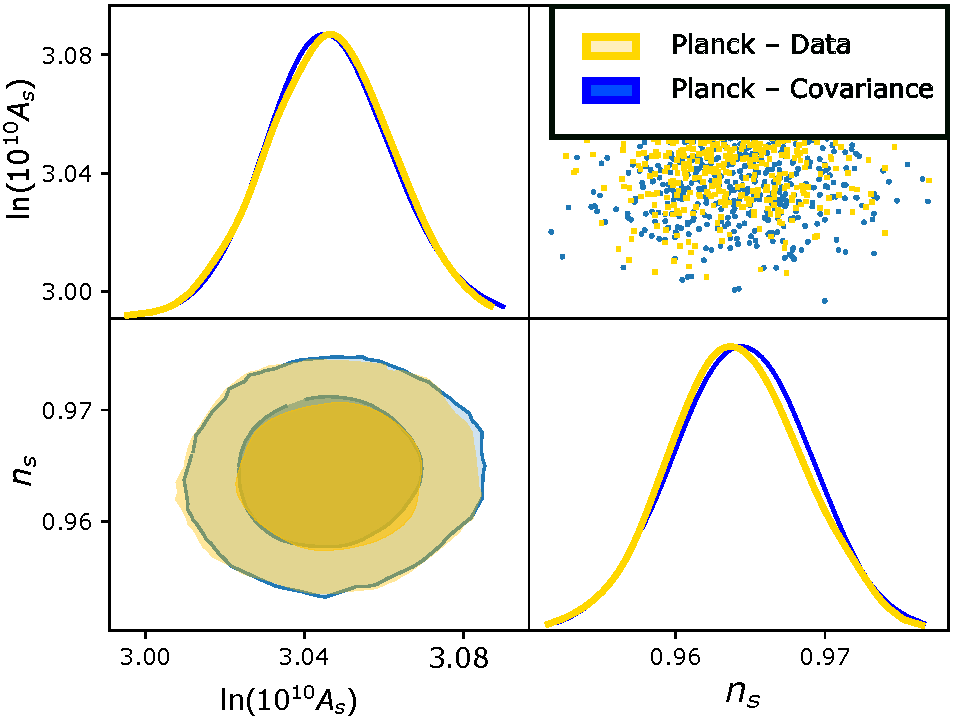
\includegraphics[width=0.5\textwidth]{./illustrations/triangle-fit.pdf}
  \caption{An example of a posterior obtained with PPR, based on
    Planck parameter covariance matrix, compared with the Planck
    posterior chains. The differences in the distributions indicate
    variance across different inference runs.
    ${\cal D}\{ {\cal P}, \bar{\cal P}\} \approx 0.01$. The deviation
    is due to a different (smaller) number of live points used, and
    the difference between the correct likelihood and its
    approximation using a Gaussian. \label{fig:overlay-posteriors}}
\end{figure}


When constructing the test cases, we shall use on no more than
three-dimensional models with Gaussian likelihoods, as they are
sufficiently general to share similarities with cosmological
inference, while also being practical to investigate under small
perturbations.  For this purpose, we use a uniform baseline prior, and
a Gaussian likelihood:
\begin{equation}
  \ln {\cal L}(\bm{\theta}) = \ln {\cal L}^\text{max}- \dfrac{1}{2}{(\bm{\theta} - \bm{\mu})}^{T}\Sigma^{-1}(\bm{\theta}-\bm{\mu}),
\end{equation}
where the covariance matrix \(\bm{\Sigma}\), specifies the extent of
the peak, and the vector \(\bm{\mu}\) --- the location.
\({\cal L}^\text{max}\) is the normalisation factor, which we keep
implicit, for convenience.

$\bm{\Sigma}$ is assumed diagonal, without loss of generality. While
$\bm{\Sigma}$ can be singular, which usually means a redundancy in the
parametrisation, which can be fixed (by turning the strongly
correlated parameters derived). Otherwise it is positive
semi-definite, and symmetric, meaning that the it can be diagonalised
via change into its eigen-basis. Counter-intuitively, this basis change must
not be made part of the quantile. It is applied before computations
involving correlated Gaussians, and reversed afterwards. This is a
consequence of the extra Jacobian brought on by the difference between
\cref{eq:partitioning} and \cref{eq:partitioning-p}. Essentially by
applying the transformation globally the unit hypercube becomes a
parallelopiped, which is the result of neglecting the Jacobian
associated to the linear transformation. 

To simulate imperfections we consider translational offsets between
the proposal prior and the model likelihood.  The main trial posterior
is thus
\begin{equation}
\bar{{\cal P}}(\bm{\theta}) = G(\bm{\theta}; \bm{\mu} =
  (1,2,3),\bm{\Sigma} = \mathds{1}_{3}),
\end{equation}
truncated to a cube of side length\footnote{The value \(1.2\) was
  chosen because it is the shortest non-machine representable floating
  point number, whose inverse is also not machine representable. This
  causes numerical instability in the uniform prior probability
  density function and quantile (at the boundaries). The value was
  chosen for tests of boundary effects, which had to be removed from
  the project, because of volume constraints. }
\(a = 1.2 \cdot 10^{9}\). The corresponding evidence (\cref{eq:def-z})
is \(\ln \mathcal{Z}\approx-62.7\). The quantile of this Gaussian
distribution is the one that enters iPPR and PPR's priors as well as
the reference likelihood. All other test cases are derived from the
same Gaussian either via re-scaling, deformation (off-diagonal
covariance and anisotropic scaling), or translation.

The choice of the prior scale: \(a = O(10^{9})\), is to ensure that
the series are not affected by run-to-run variance, even with a
reduced number of live points. This has the added benefit of
simulating an unbounded uniform prior numerically, as it is near the
numerical limits. Also, any error in re-scaling the likelihood
(e.g.~\cref{fig:hist}) leading to an inconsistent partition would not
be obvious or as clean with a smaller prior boundary. Lastly, this
choice allowed us to test the hypothesis that both stochastic mixtures
and power posterior repartitioning can effectively remove the burn-in
stage altogether. Last but not least, with such preconditions,
stochastic mixtures are put at the greatest disadvantage. In the
average case, approximately half the original live points are drawn
from the proposal distribution and half from the uniform. The
probability of finding the offset posterior peak is thus minuscule for
large offsets. By contrast, In the average case the original live
points with a Gaussian power posterior are drawn from a twice broad
Gaussian.



\section{Results and Discussion.}\label{sec:results}
The first test was to ensure that the repartitioning was implemented
correctly. For this goal, we produced coinciding Gaussian likelihoods
and prior components. The results of the test are shown in
\cref{tab:hist} and \cref{fig:hist}.


The second class of tests involved deforming the prior Gaussians.
Both SSIM (iPPR and uniform) and PPR were resilient with respect to
re-scaling and anisotropic deformation of the likelihood, obtaining
${\cal D}\{ {\cal P}, \bar{\cal P}\} \leq 0.03$. iPPR coped with
situations where ${\cal P}$ was narrower than $\pi$, while failing in
the opposite case: ${\cal D}\{ {\cal P}, \bar{\cal P}\} \geq 5.5$,
when ${\cal D}\{ \pi, {\cal P} \} = 5.5$ and
$\Sigma = 0.3 \times \mathds{1}_{3}$.

The final test was with regards to translational offsets. The results
are shown in \cref{fig:kl-d,fig:convergence,fig:drift}. In
\cref{fig:kl-d}, we see that the amount of information extracted from
PPR increases with increased offset. However, it does so sub-linearly,
which combined with \cref{fig:convergence}, renders suspect the
validity of the posteriors obtained using PPR and SSIM. However,
\cref{fig:drift} shows that only PPR is adversely affected.

The posterior to posterior Kullback-Leibler divergence remained stable
and less than \(0.3\) for the stochastic mixture and the
reference. Power repartitioning fluctuated considerably, ensuring that
no suitable plot could be produced. This suggests instability with respect to
perturbations, and unpredictability of the accuracy of the
posterior. However, none of the values reached the prior to posterior
divergence, suggesting that at no offset was the posterior entirely
obtained from the prior. As a result, power repartitioning may still
be useful for unrepresentative informative priors, that are not
proposals, as \cite{chen-ferroz-hobson} have shown.

A special case is that shown in \cref{fig:convergence}, in a reduced
size bounding box \(a=2\times 10^{3}\). The main notable feature is
the inaccuracy of the posterior obtained by PPR. If the offset is
small --- \(O(2\sigma)\), the posterior is shifted. With a larger
offset, e.g. \(O(4\sigma)\), two peaks can be resolved.  Both errors
are caused by incorrect evidence (see \cref{fig:drift}) PPR:
\(\ln {\cal Z}\approx -25.4 \pm 2\), vs uniform reference
\(\ln {\cal Z} = -22.7 \pm 0.4\) and SSIM,
\(\ln {\cal Z} = -22.5 \pm 0.3\). There are two key observations to be
made: the evidence is still within reasonable variance from the
reference, and its estimated error is large. As a result, while we
haven't obtained the right information, we know that something went
wrong.

This result is not at variance with \cite{chen-ferroz-hobson}'s
observations, as they do not have a comparable test case. All of their
numerical test cases were restricted to no more than two physical
parameters, while we extended it to three. The example given required
considerable fine-tuning to be reproducible\footnote{Too much free
  time in quarantine. }, as larger or smaller offsets often lead to
correct convergence some of the time. Another hint at why power
repartitioning may have been affected more than a stochastic mixture
can be gleaned from \cref{fig:hist}. By noticing that the correct
evidence is still within one standard deviation of the estimate
obtained using power repartitioning we can suggest, that the result is
less precise. So the unusual shape of the marginalised posterior, is
the result of loss of precision. The inaccurate posterior is within
margin of error of the analytical result,


\begin{figure}
  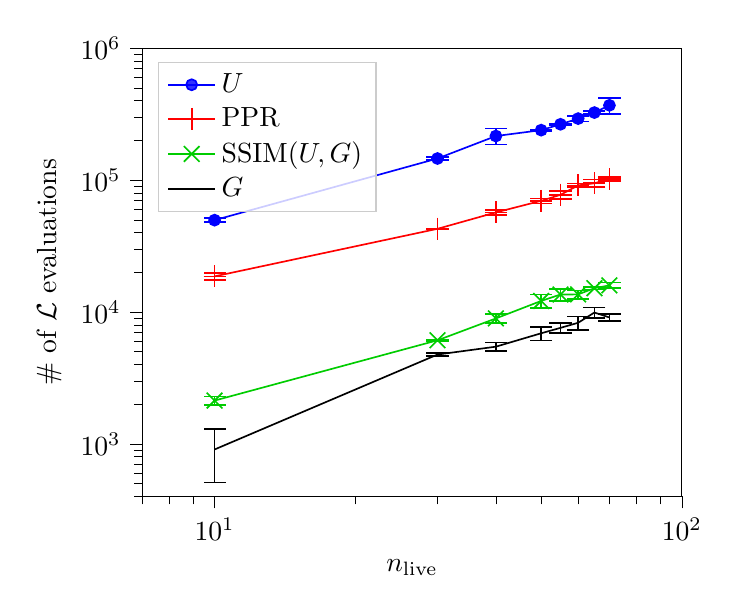
\begin{tikzpicture}

\definecolor{color0}{rgb}{0.0,0.0,1.0} %U
\definecolor{color1}{rgb}{1,0.0,0.0} %PPR
\definecolor{color2}{rgb}{0,0.8,0.0}                              %SSIM
\definecolor{color3}{rgb}{0.,0.0,0.0} %G

\begin{axis}[
legend cell align={left},
legend style={fill opacity=0.8, draw opacity=1, text opacity=1, at={(0.03,0.97)}, anchor=north west, draw=white!80!black},
tick align=outside,
tick pos=left,
x grid style={white!69.0196078431373!black},
xlabel={\(n_\text{live}\)},
xmin=7, xmax=100,
xtick style={color=black},
y grid style={white!69.0196078431373!black},
ylabel={\# of \({\cal L}\) evaluations},
ymin=400, ymax=1000000.0,
ytick style={color=black},
xmode=log,
ymode=log
]
\path [draw=color0, semithick]
(axis cs:10,48051.1762746562)
--(axis cs:10,51361.4903920105);

\path [draw=color0, semithick]
(axis cs:30,141787.579248368)
--(axis cs:30,149701.087418299);

\path [draw=color0, semithick]
(axis cs:40,185671.527674282)
--(axis cs:40,245784.472325718);

\path [draw=color0, semithick]
(axis cs:50,236296.832694899)
--(axis cs:50,241822.500638435);

\path [draw=color0, semithick]
(axis cs:55,262655.71356965)
--(axis cs:55,266952.953097016);

\path [draw=color0, semithick]
(axis cs:60,278243.015081106)
--(axis cs:60,306644.984918894);

\path [draw=color0, semithick]
(axis cs:65,317116.521541605)
--(axis cs:65,332736.145125062);

\path [draw=color0, semithick]
(axis cs:70,318358.948415036)
--(axis cs:70,419081.71825163);

\path [draw=color1, semithick]
(axis cs:10,17520.6487596482)
--(axis cs:10,19742.0179070185);

\path [draw=color1, semithick]
(axis cs:30,42472.9620658463)
--(axis cs:30,42994.371267487);

\path [draw=color1, semithick]
(axis cs:40,54281.6999405287)
--(axis cs:40,59494.3000594713);

\path [draw=color1, semithick]
(axis cs:50,66559.0160569084)
--(axis cs:50,72717.6506097582);

\path [draw=color1, semithick]
(axis cs:55,71552.6011973656)
--(axis cs:55,83118.7321359677);

\path [draw=color1, semithick]
(axis cs:60,88312.8386239607)
--(axis cs:60,94072.4947093726);

\path [draw=color1, semithick]
(axis cs:65,88215.9096228476)
--(axis cs:65,100992.090377152);

\path [draw=color1, semithick]
(axis cs:70,97882.04633)
--(axis cs:70,105637.95367);

\path [draw=color2, semithick]
(axis cs:10,1980.99743591911)
--(axis cs:10,2284.33589741422);

\path [draw=color2, semithick]
(axis cs:30,6035.87692136486)
--(axis cs:30,6174.12307863514);

\path [draw=color2, semithick]
(axis cs:40,8260.41435100755)
--(axis cs:40,9624.91898232578);

\path [draw=color2, semithick]
(axis cs:50,10733.0849396109)
--(axis cs:50,13538.9150603891);

\path [draw=color2, semithick]
(axis cs:55,12122.9645002052)
--(axis cs:55,15015.0354997948);

\path [draw=color2, semithick]
(axis cs:60,12622.7721075812)
--(axis cs:60,14593.2278924188);

\path [draw=color2, semithick]
(axis cs:65,14804.9685728395)
--(axis cs:65,15505.0314271605);

\path [draw=color2, semithick]
(axis cs:70,15158.1193669152)
--(axis cs:70,16693.8806330848);

\path [draw=color3, semithick]
(axis cs:10,511.628293172651)
--(axis cs:10,1305.03837349402);

\path [draw=color3, semithick]
(axis cs:30,4625.34584399058)
--(axis cs:30,4900.65415600942);

\path [draw=color3, semithick]
(axis cs:40,5045.39013421616)
--(axis cs:40,5880.60986578384);

\path [draw=color3, semithick]
(axis cs:50,6085.69651897324)
--(axis cs:50,7719.6368143601);

\path [draw=color3, semithick]
(axis cs:55,6959.0338647499)
--(axis cs:55,8215.63280191676);

\path [draw=color3, semithick]
(axis cs:60,7317.2571539732)
--(axis cs:60,9267.40951269347);

\path [draw=color3, semithick]
(axis cs:65,8986.02980736454)
--(axis cs:65,10838.6368593021);

\path [draw=color3, semithick]
(axis cs:70,8588.48027282128)
--(axis cs:70,9612.18639384539);


\addplot [semithick, color1, mark=-, mark size=4, mark options={solid}, only marks, forget plot]
table {%
10 17520.6487596482
30 42472.9620658463
40 54281.6999405287
50 66559.0160569084
55 71552.6011973656
60 88312.8386239607
65 88215.9096228476
70 97882.04633
};
\addplot [semithick, color1, mark=-, mark size=4, mark options={solid}, only marks, forget plot]
table {%
10 19742.0179070185
30 42994.371267487
40 59494.3000594713
50 72717.6506097582
55 83118.7321359677
60 94072.4947093726
65 100992.090377152
70 105637.95367
};
\addplot [semithick, color2, mark=-, mark size=4, mark options={solid}, only marks, forget plot]
table {%
10 1980.99743591911
30 6035.87692136486
40 8260.41435100755
50 10733.0849396109
55 12122.9645002052
60 12622.7721075812
65 14804.9685728395
70 15158.1193669152
};
\addplot [semithick, color2, mark=-, mark size=4, mark options={solid}, only marks, forget plot]
table {%
10 2284.33589741422
30 6174.12307863514
40 9624.91898232578
50 13538.9150603891
55 15015.0354997948
60 14593.2278924188
65 15505.0314271605
70 16693.8806330848
};
\addplot [semithick, color3, mark=-, mark size=4, mark options={solid}, only marks, forget plot]
table {%
10 511.628293172651
30 4625.34584399058
40 5045.39013421616
50 6085.69651897324
55 6959.0338647499
60 7317.2571539732
65 8986.02980736454
70 8588.48027282128
};
\addplot [semithick, color3, mark=-, mark size=4, mark options={solid}, only marks, forget plot]
table {%
10 1305.03837349402
30 4900.65415600942
40 5880.60986578384
50 7719.6368143601
55 8215.63280191676
60 9267.40951269347
65 10838.6368593021
70 9612.18639384539
};
\addplot [semithick, color0, mark=-, mark size=4, mark options={solid}, only marks, forget plot]
table {%
10 48051.1762746562
30 141787.579248368
40 185671.527674282
50 236296.832694899
55 262655.71356965
60 278243.015081106
65 317116.521541605
70 318358.948415036
};
\addplot [semithick, color0, mark=-, mark size=4, mark options={solid}, only marks, forget plot]
table {%
10 51361.4903920105
30 149701.087418299
40 245784.472325718
50 241822.500638435
55 266952.953097016
60 306644.984918894
65 332736.145125062
70 419081.71825163
};
\addplot [semithick, color0, mark=*, mark size=2, mark options={solid}]
table {%
10 49706.3333333333
30 145744.333333333
40 215728
50 239059.666666667
55 264804.333333333
60 292444
65 324926.333333333
70 368720.333333333
};
\addlegendentry{$U$}
\addplot [semithick, color1, mark=+, mark size=4, mark options={solid}]
table {%
10 18631.3333333333
30 42733.6666666667
40 56888
50 69638.3333333333
55 77335.6666666667
60 91192.6666666667
65 94604
70 101760
};
\addlegendentry{PPR}
\addplot [semithick, color2, mark=x, mark size=4, mark options={solid}]
table {%
10 2132.66666666667
30 6105
40 8942.66666666667
50 12136
55 13569
60 13608
65 15155
70 15926
};
\addlegendentry{$\text{SSIM}(U,G)$}
\addplot [semithick, color3, mark=., mark size=2, mark options={solid}]
table {%
10 908.333333333333
30 4763
40 5463
50 6902.66666666667
55 7587.33333333333
60 8292.33333333333
65 9912.33333333333
70 9100.33333333333
};
\addlegendentry{$G$}
\end{axis}

\end{tikzpicture}

  \caption{number of ${\cal L}$ evaluations as a function of the
    number of live points. \(U\) is the reference uniform, and \(G\)
    is the pure Gaussian proposal.
    \(\max {\cal D}\{{\cal P}, \bar{\cal P}\} < 1.5\), meaning all
    participating consistent partitions obtained the correct
    posterior. The number of evaluations scales as
    $k\cdot n_\text{live}^{1.1 \pm 0.2}$, where $k$ reduces for faster
    repartitioning schemes. \label{fig:benchmark}}
\end{figure}


It is worthwhile to consider the impact of such a scenario occurring
during practical use of Bayesian inference. If either of the posterior
looks as PPR's marginalised posteriors in \cref{fig:convergence}, the
researcher performing the inference has the following options:
\begin{enumerate}
\item accept the posterior as is~\label[Option]{opt:accept}
\item accept the posterior, but as a less credible result\label[Option]{opt:accept-with-err}
\item reject the PPR result entirely, and perform a run with only a
uniform prior\label[Option]{opt:uniform}
\item readjust the PPR mean and variance using the posterior, and
re-run~\label[Option]{opt:shift}
\item combine PPR with SSIM in mixture with a uniform prior
\end{enumerate}
\Cref{opt:accept-with-err} is a last resort. \Cref{opt:accept} is
adequate for low accuracy applications, provided errors are properly
estimated using e.g.~\texttt{nestcheck} \citep{higson2018nestcheck}.
From \cref{fig:benchmark}, we see that the performance uplift allows
for \cref{opt:shift} to be more efficient than~\ref{opt:uniform},
albeit marginally so.

This is where our technique is most useful: one obtains, as we've
shown in~\cref{fig:convergence}, a more accurate
\({\cal P}(\bm{\theta})\), by using PPR from within SSIM. Hence, a
repartitioning scheme that is on average slower than PPR (by
approximately \(18\%\) extra \({\cal L}\) evaluations) within margin
of run-to-run variance of PPR (approximately
\(20\%\))\footnote{Comparison with \cref{fig:benchmark} may be
  misleading, as the error margins there correspond to exact
  coincidence, while the case in question involves an offset of
  $6\mu$. }, which is an order of magnitude less
than~\vref{opt:uniform,opt:shift} would afford. That said, using the
proposal directly is faster still \cref{fig:benchmark}.

\begin{figure}
  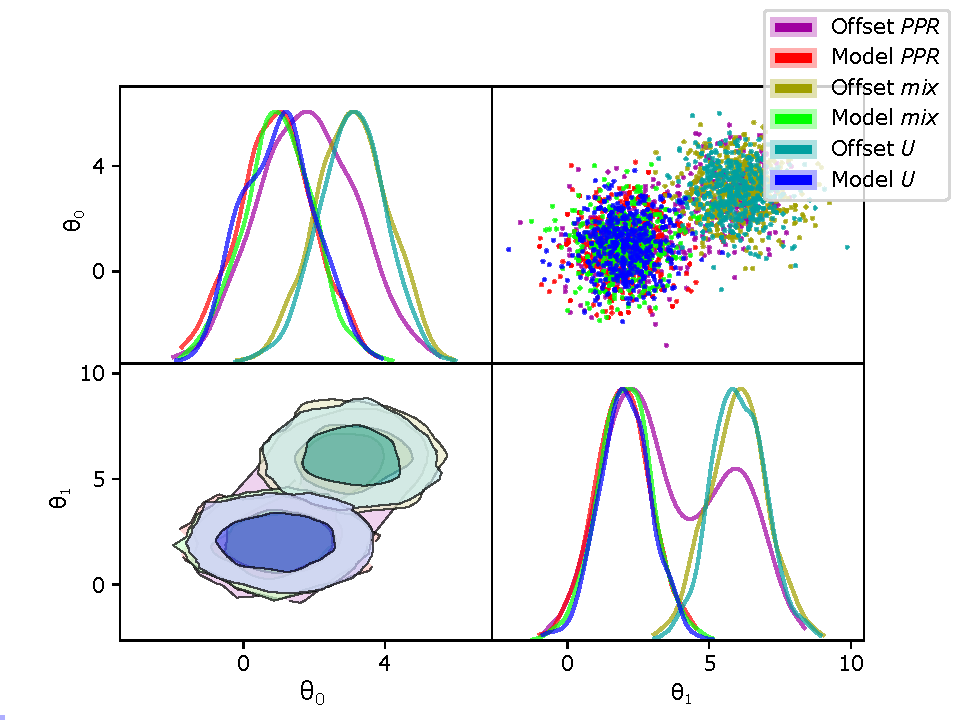
\includegraphics[width=0.99\columnwidth]{./illustrations/convergence.pdf}
  \caption{An illustration of offsets affecting ${\cal P}$ under
    various repartitioning schemes. Dotted series represent the prior
    imprint. The reference uniform and the stochastic mixture agree
    with the analytical posterior: Gaussian peak at
    $\bm{\theta} = (4, 6, 8)$. \label{fig:convergence}}
\end{figure}

\begin{figure} \centering
  \begin{subfigure}{0.99\columnwidth}
    \centering

    % This file was created by tikzplotlib v0.9.1.
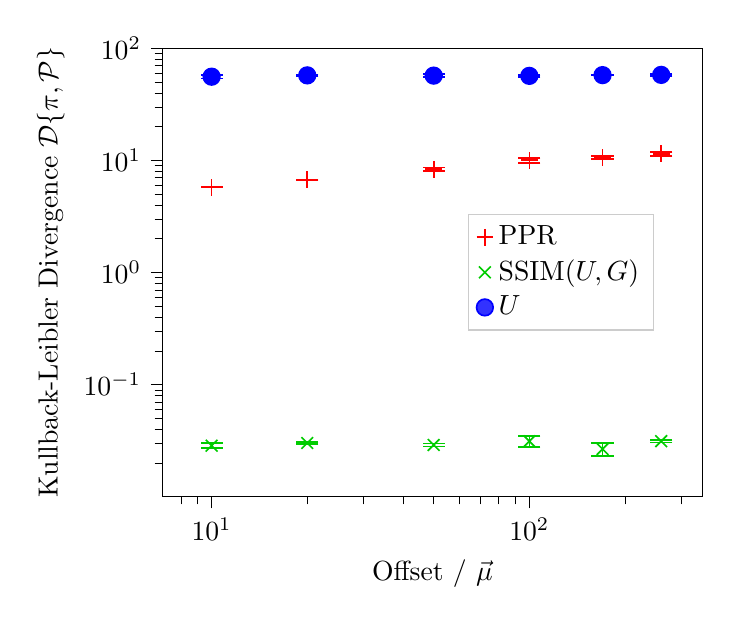
\begin{tikzpicture}

\definecolor{color0}{rgb}{1,0.0,0.0} %ppr
\definecolor{color1}{rgb}{0,0.8,0.0} %mix
\definecolor{color2}{rgb}{0.0,0.0,1.0} %U

\begin{axis}[
legend cell align={left},
legend style={fill opacity=0.8, draw opacity=1, text opacity=1, at={(0.91,0.5)}, anchor=east, draw=white!80!black},
tick align=outside,
tick pos=left,
x grid style={white!69.0196078431373!black},
xlabel={Offset / \(\displaystyle \vec{\mu}\)},
xmin=-3.0, xmax=350.0,
xtick style={color=black},
y grid style={white!69.0196078431373!black},
ylabel={Kullback-Leibler Divergence \(\displaystyle {\cal D}\{\pi, {\cal P}\}\)},
ymin=-3.0, ymax=100.0,
ytick style={color=black},
xmode=log,
ymode=log
]
\path [draw=color0, semithick]
(axis cs:10,5.71795365099151)
--(axis cs:10,5.77133948534581);

\path [draw=color0, semithick]
(axis cs:20,6.6768824419002)
--(axis cs:20,6.77321107556694);

\path [draw=color0, semithick]
(axis cs:50,8.02877279045042)
--(axis cs:50,8.63543918622054);

\path [draw=color0, semithick]
(axis cs:100,9.52185212376919)
--(axis cs:100,10.4908349952443);

\path [draw=color0, semithick]
(axis cs:170,10.3029683750536)
--(axis cs:170,10.9155451202318);

\path [draw=color0, semithick]
(axis cs:260,10.954510866509)
--(axis cs:260,11.9335782130671);

\path [draw=color1, semithick]
(axis cs:10,0.0271909650803472)
--(axis cs:10,0.030089733601838);

\path [draw=color1, semithick]
(axis cs:20,0.029683008672791)
--(axis cs:20,0.0308036500189849);

\path [draw=color1, semithick]
(axis cs:50,0.0282101242046804)
--(axis cs:50,0.0298855157628486);

\path [draw=color1, semithick]
(axis cs:100,0.0278177027329167)
--(axis cs:100,0.0348526563256524);

\path [draw=color1, semithick]
(axis cs:170,0.0232802581598788)
--(axis cs:170,0.0301604324600733);

\path [draw=color1, semithick]
(axis cs:260,0.0304771056975755)
--(axis cs:260,0.0323746358923458);

\path [draw=color2, semithick]
(axis cs:10,53.6407046096139)
--(axis cs:10,57.7293889288474);

\path [draw=color2, semithick]
(axis cs:20,56.1280894679801)
--(axis cs:20,58.3022565457241);

\path [draw=color2, semithick]
(axis cs:50,55.3633380690649)
--(axis cs:50,58.47445725549);

\path [draw=color2, semithick]
(axis cs:100,55.5223746731559)
--(axis cs:100,57.7271641567295);

\path [draw=color2, semithick]
(axis cs:170,56.8924880373743)
--(axis cs:170,58.1261131182599);

\path [draw=color2, semithick]
(axis cs:260,56.3603430284318)
--(axis cs:260,59.2024246504929);

\addplot [semithick, color0, mark=-, mark size=4, mark options={solid}, only marks, forget plot]
table {%
10 5.71795365099151
20 6.6768824419002
50 8.02877279045042
100 9.52185212376919
170 10.3029683750536
260 10.954510866509
};
\addplot [semithick, color0, mark=-, mark size=4, mark options={solid}, only marks, forget plot]
table {%
10 5.77133948534581
20 6.77321107556694
50 8.63543918622054
100 10.4908349952443
170 10.9155451202318
260 11.9335782130671
};
\addplot [semithick, color1, mark=-, mark size=4, mark options={solid}, only marks, forget plot]
table {%
10 0.0271909650803472
20 0.029683008672791
50 0.0282101242046804
100 0.0278177027329167
170 0.0232802581598788
260 0.0304771056975755
};
\addplot [semithick, color1, mark=-, mark size=4, mark options={solid}, only marks, forget plot]
table {%
10 0.030089733601838
20 0.0308036500189849
50 0.0298855157628486
100 0.0348526563256524
170 0.0301604324600733
260 0.0323746358923458
};
\addplot [semithick, color2, mark=-, mark size=4, mark options={solid}, only marks, forget plot]
table {%
10 53.6407046096139
20 56.1280894679801
50 55.3633380690649
100 55.5223746731559
170 56.8924880373743
260 56.3603430284318
};
\addplot [semithick, color2, mark=-, mark size=4, mark options={solid}, only marks, forget plot]
table {%
10 57.7293889288474
20 58.3022565457241
50 58.47445725549
100 57.7271641567295
170 58.1261131182599
260 59.2024246504929
};
\addplot [semithick, color0, mark=+, mark size=3, mark options={solid}, only marks]
table {%
10 5.74464656816866
20 6.72504675873357
50 8.33210598833548
100 10.0063435595067
170 10.6092567476427
260 11.4440445397881
};
\addlegendentry{PPR}
\addplot [semithick, color1, mark=x, mark size=3, mark options={solid}, only marks]
table {%
10 0.0286403493410926
20 0.0302433293458879
50 0.0290478199837645
100 0.0313351795292845
170 0.026720345309976
260 0.0314258707949607
};
\addlegendentry{SSIM$(U,G)$}
\addplot [semithick, color2, mark=*, mark size=3, mark options={solid}, only marks]
table {%
10 55.6850467692306
20 57.2151730068521
50 56.9188976622774
100 56.6247694149427
170 57.5093005778171
260 57.7813838394624
};
\addlegendentry{$U$}
\end{axis}

\end{tikzpicture}

    \caption{Kullback-Leibler divergence \({\cal D}\) for different
      offsets: Gaussian peaks displaced from \(\bm{\mu}\) by
      \(\text{Offset}\times \bm{\mu}\). Notice that the faster
      repartitioning methods produce a lower value of \({\cal
        D}\). The divergence \({\cal D}\) scales sub-linearly with the
      offset.\label{fig:kl-d}}
\end{subfigure}

\begin{subfigure}{0.99\columnwidth}
  \centering

  % This file was created by tikzplotlib v0.9.1.
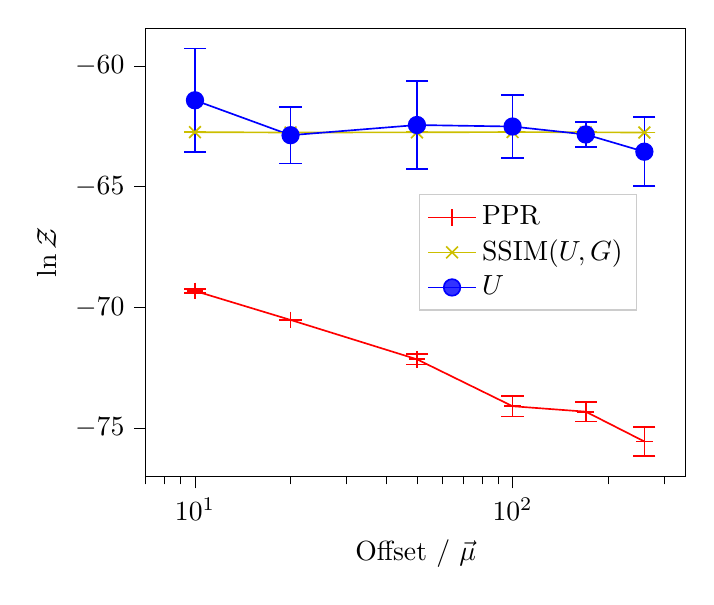
\begin{tikzpicture}

\definecolor{color0}{rgb}{1,0.0,0.0}
\definecolor{color1}{rgb}{0.8,0.75,0.0}
\definecolor{color2}{rgb}{0.0,0.0,1}

\begin{axis}[
legend cell align={left},
legend style={fill opacity=0.8, draw opacity=1, text opacity=1, at={(0.91,0.5)}, anchor=east, draw=white!80!black},
tick align=outside,
tick pos=left,
x grid style={white!69.0196078431373!black},
xlabel={Offset / \(\displaystyle \vec{\mu}\)},
xmin=-2.5, xmax=350.5,
xtick style={color=black},
y grid style={white!69.0196078431373!black},
ylabel={\(\displaystyle \ln {\cal Z}\)},
ymin=-77.013439988999, ymax=-58.4325947574349,
ytick style={color=black},
xmode=log
]
\path [draw=color0, semithick]
(axis cs:10,-69.4059960469118)
--(axis cs:10,-69.2379297037398);

\path [draw=color0, semithick]
(axis cs:20,-70.5299156173721)
--(axis cs:20,-70.5157474991409);

\path [draw=color0, semithick]
(axis cs:50,-72.3755951664078)
--(axis cs:50,-71.9328145858461);

\path [draw=color0, semithick]
(axis cs:100,-74.5305277482911)
--(axis cs:100,-73.6673769114354);

\path [draw=color0, semithick]
(axis cs:170,-74.7380053024013)
--(axis cs:170,-73.9121550603194);

\path [draw=color0, semithick]
(axis cs:260,-76.168856114837)
--(axis cs:260,-74.9518470928008);

\path [draw=color1, semithick]
(axis cs:10,-62.7439928102151)
--(axis cs:10,-62.7359696372663);

\path [draw=color1, semithick]
(axis cs:20,-62.755485458383)
--(axis cs:20,-62.7535773275597);

\path [draw=color1, semithick]
(axis cs:50,-62.7484141957878)
--(axis cs:50,-62.7468638775576);

\path [draw=color1, semithick]
(axis cs:100,-62.7369486572665)
--(axis cs:100,-62.7333125352419);

\path [draw=color1, semithick]
(axis cs:170,-62.746863877575)
--(axis cs:170,-62.745391448683);

\path [draw=color1, semithick]
(axis cs:260,-62.7574960930232)
--(axis cs:260,-62.7517661617973);

\path [draw=color2, semithick]
(axis cs:10,-63.5623386499016)
--(axis cs:10,-59.2771786315969);

\path [draw=color2, semithick]
(axis cs:20,-64.0348662974579)
--(axis cs:20,-61.6973543628668);

\path [draw=color2, semithick]
(axis cs:50,-64.2749108611421)
--(axis cs:50,-60.6135450768888);

\path [draw=color2, semithick]
(axis cs:100,-63.8144479355573)
--(axis cs:100,-61.1997313352197);

\path [draw=color2, semithick]
(axis cs:170,-63.3536082125541)
--(axis cs:170,-62.3180044247467);

\path [draw=color2, semithick]
(axis cs:260,-64.9781441262723)
--(axis cs:260,-62.1236339929356);

\addplot [semithick, color0, mark=-, mark size=4, mark options={solid}, only marks, forget plot]
table {%
10 -69.4059960469118
20 -70.5299156173721
50 -72.3755951664078
100 -74.5305277482911
170 -74.7380053024013
260 -76.168856114837
};
\addplot [semithick, color0, mark=-, mark size=4, mark options={solid}, only marks, forget plot]
table {%
10 -69.2379297037398
20 -70.5157474991409
50 -71.9328145858461
100 -73.6673769114354
170 -73.9121550603194
260 -74.9518470928008
};
\addplot [semithick, color1, mark=-, mark size=4, mark options={solid}, only marks, forget plot]
table {%
10 -62.7439928102151
20 -62.755485458383
50 -62.7484141957878
100 -62.7369486572665
170 -62.746863877575
260 -62.7574960930232
};
\addplot [semithick, color1, mark=-, mark size=4, mark options={solid}, only marks, forget plot]
table {%
10 -62.7359696372663
20 -62.7535773275597
50 -62.7468638775576
100 -62.7333125352419
170 -62.745391448683
260 -62.7517661617973
};
\addplot [semithick, color2, mark=-, mark size=4, mark options={solid}, only marks, forget plot]
table {%
10 -63.5623386499016
20 -64.0348662974579
50 -64.2749108611421
100 -63.8144479355573
170 -63.3536082125541
260 -64.9781441262723
};
\addplot [semithick, color2, mark=-, mark size=4, mark options={solid}, only marks, forget plot]
table {%
10 -59.2771786315969
20 -61.6973543628668
50 -60.6135450768888
100 -61.1997313352197
170 -62.3180044247467
260 -62.1236339929356
};
\addplot [semithick, color0, mark=+, mark size=3, mark options={solid}]
table {%
10 -69.3219628753258
20 -70.5228315582565
50 -72.154204876127
100 -74.0989523298633
170 -74.3250801813604
260 -75.5603516038189
};
\addlegendentry{PPR}
\addplot [semithick, color1, mark=x, mark size=3, mark options={solid}]
table {%
10 -62.7399812237407
20 -62.7545313929713
50 -62.7476390366727
100 -62.7351305962542
170 -62.746127663129
260 -62.7546311274102
};
\addlegendentry{SSIM$(U, G)$}
\addplot [semithick, color2, mark=*, mark size=3, mark options={solid}]
table {%
10 -61.4197586407493
20 -62.8661103301623
50 -62.4442279690155
100 -62.5070896353885
170 -62.8358063186504
260 -63.5508890596039
};
\addlegendentry{$U$}
\end{axis}

\end{tikzpicture}

  
  \caption{An illustration of offsets affecting ${\cal Z}$. The true
    value is constant, mirrored by the mixture: SSIM of PPR and
    reference uniform. PPR alone produces incorrect evidence,
    consistent with \cref{fig:convergence}. Tighter error-bars on SSIM
    are consistent with our observations from
    \cref{fig:hist}.\label{fig:drift}}
\end{subfigure}
\caption{Illustrations of effects of offsets on the correctness
  \ref{fig:drift} and performance \ref{fig:kl-d} of nested sampling
  under consistent posterior repartitioning.}
\end{figure}



Lastly, \textbf{\emph{posterior mass}} --- a measure of convergence
speed \citep{higson2018nestcheck}, is often used in diagnosing nested
sampling. Typical examples of posterior mass for a run with
$\pi=\text{Const.}$ and runs accelerated by posterior repartitioning
are given in \cref{fig:higson}. Notice that the re-partitioned series
has a longer extinction phase, as a result of introducing extra
nuisance parameters. Also, the confidence intervals on each parameter
between the uniform and the re-partitioned run are identical,
signifying that we have not lost precision.

\begin{figure*}
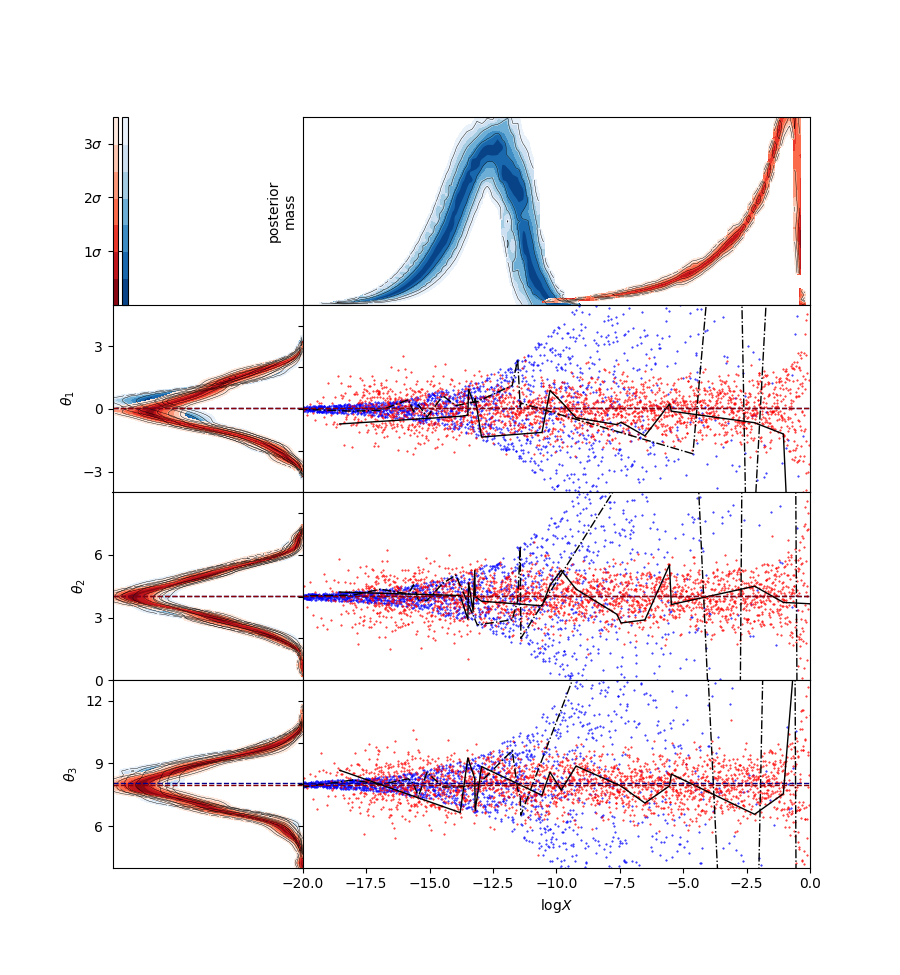
\includegraphics[width=.99\textwidth]{./illustrations/higson.png}
\caption{plot of the evolution of nested sampling. The \color{red} red
  \color{black} series corresponds to SSIM of iPPR, while the
  \color{blue} blue \color{black} series --- to a reference
  uniform. The horizontal axis of plots in the second column is
  \(\ln X\), where \(X(\mathcal{L}) \in [0,1]\) is the fraction of the
  prior with likelihood greater than \(\mathcal{L}\). The top plot is
  the relative posterior mass. In row $i$ the ${\cal P}(\theta_{i})$
  is plotted. Confidence intervals represented with color
  intensity. The reference values for the model parameters are
  \(\theta = (0, 4, 8)\) \label{fig:higson}}
\end{figure*}

\subsection{Cosmological Simulations.}\label{sec:orgb81c159}
After an initial run of \texttt{Cobaya} \citep{cobaya}, we have obtained the marginalised
posteriors of all the key parameters of the \(\Lambda\)CDM model,
as well as the nuisance parameters.

First, we have performed an inference using the Planck \citep{Planck} dataset,
with the \(\Lambda\)CDM model. The results of our initial run are
presented in \cref{fig:cosmology}. From these data, under the
assumption that the parameters' posteriors are a correlated Gaussian
distribution, we extract the means $\bm{\mu}$ and the covariance
matrix \(\bm{\Sigma}\).

We use a stochastic mixture of a uniform prior and a single Gaussian
obtained from the posterior samples of a run with a uniform prior,
which we patch into \texttt{Cobaya}'s interface to \texttt{PolyChord}
\citep{code}. The posteriors of two runs with identical settings (save
live point number) are given in \cref{fig:cosmology}.

Firstly, notice that the posteriors have a significant overlap. Each
plot on the diagonal of \cref{fig:cosmology} is a Gaussian, agreeing
with the results of the reference run to within less than 1/10$^{th}$ of a
standard deviation. However SSIM predicts a deformed (non-ellipsoidal)
covariance of the \(\Lambda\)CDM parameters. 

The deformations are present in all posteriors that used a Gaussian
proposal, which indicates that the deformations are systematic. The
deformities are not caused by finite-grain size in the stochastic
mixture, as the Gaussian proposal has them, and to a greater
extent. The mixing portion parameter $\beta$, has converged to a mean
of $\langle \beta \rangle = 0.82$, which indicates that the Gaussian
proposal was not fully the most representative, but also that the
later stages of sampling were dominated by the Gaussian
proposal. Despite the appearance, however, \cref{tab:cosmo-accuracy}
shows that the posteriors between SSIM and non-SSIM runs are not
significantly different (${\cal D}< 0.3$). Moreover the evidence is
within one standard deviation and more precise with SSIM by a factor
of \(8\).

While this might indicate a higher accuracy than obtainable with a
pure uniform prior, one must exercise caution. While we can eliminate
some potential systematic errors, a more conclusive analysis is
needed.

With accuracy out of the way, \cref{tab:cosmo-performance}, highlights
a significant improvement in performance. Using SSIM offers a
reduction of run-time by a factor of \(19\). By exploiting increased
precision one can reduce the number of live points, and gain a further
reduction of run-time by a factor of \(37\). Further improvements are
attainable by reducing the precision criterion and terminating
early. Conversely, to obtain similar precision to SSIM, assuming
sub-linear scaling with \(n_\text{live}\), one would need to extend
the duration of the inference to 912 hours \(\approx\) 40
days. Assuming that errors in evidence scale as
\(n_\text{live}^{-1/2}\) the time would be then of the order of a
year.




\begin{table}
  \centering
  \caption{Accuracy metrics for Cosmology runs using Cobaya.}
  \begin{tabular}{llrrr}
    \textbf{Prior} & \textbf{Device} & ${\cal D}\{ {\cal P}, \bar{\cal P}\}$ & $\ln {\cal Z}$ & $n_\text{live}$\\
    \hline
    Uniform & CSD3 &\( 0.000\) & \(-1432.8 \pm 0.8\) & 108\\
    SSIM\((U, G)\) & CSD3 & \(0.2\) & \(-1433.6 \pm 0.1\) & 100\\
    iPPR(\(G\)) & CSD3 & \(0.4\) & \(-1433.8 \pm 0.05\) & 100\\
    SSIM\((U, G)\) & PC & \(0.25\) & \(-1433.5 \pm 0.2\) & 50
  \end{tabular}
  \label{tab:cosmo-accuracy}
\end{table}

\begin{table}
  \centering
  \caption{Performance metrics for Cosmology runs using Cobaya. $t$ is
    the time from beginning of sampling, to output. Starred series
    were extrapolated linearly. Precision normalisation assumes errors in
    ${\cal Z}$ scale as $n_\text{live}^{-1}$. }
  \begin{tabular}{llrrr}
    \textbf{Prior} & \textbf{Device used} & \textbf{$t$/(hrs)} & \({\cal N}\{ {\cal L}\}\) & $n_\text{live}$\\
    \hline
    Uniform & CSD3 &\( 32.2 \) & \(480 000\) & 108\\
    SSIM\((U, G)\) & CSD3 & \(1.7\) & \(90 000\) & 100\\
    SSIM\((U, G)\) & PC & \(50\) & \(49 000\) & 50\\
    \hline
    Uniform & PC$^{*}$ & \(912\) & \(240 000\) & 50\\
    Uniform & CSD3$^{*}$ &  \(224\) & 3 360 000  & 700
  \end{tabular}
  \label{tab:cosmo-performance}
\end{table}

\section{Conclusions}\label{sec:orgdf2cbd9}

\subsection{Results}\label{sec:orgc48c55d}
The project's purpose has been to investigate the performance increase
attainable by algorithmic optimisations of the inputs to nested
sampling.We have identified a class of methods based on work by
\cite{chen-ferroz-hobson}, called consistent partitions, fit for this
purpose. We have shown that each consistent partition can accelerate
nested sampling when given an informative proposal.  We have developed
stochastic superpositional isometric mixing (SSIM), to combine several
proposals, into one. When used with nested sampling, SSIM produces
more precise and accurate posteriors, faster than any individual
consistent partition.

We have established the following advantages in using SSIM over PPR:
SSIM admits multiple types of proposal priors, while PPR admits only
one; it permits a broader class of proposals, for example: with
differing domains, while PPR --- only if the domains of the proposals
coincide.  SSIM is abstract: the prior quantile is a superposition of
the constituent priors' quantiles. By contrast, PPR prior quantile
needs to be calculated by the end user for each type of proposal. The
calculation is non-trivial for non-Gaussian proposals. SSIM supports
an unbiased reference (uniform) prior exactly. PPR tends to an
unbiased reference as \(\beta\rightarrow 0 \), but is only truly
unbiased if $\beta=0$, with negligible probability. SSIM, like PPR,
prefers the prior that leads to a higher likelihood, but unlike PPR,
this does not lead to the total exclusion of less-representative
priors.


As a result, faster, but more fragile consistent partitions
(e.g.~iPPR), in conjunction with a standard uniform prior can exceed
more robust but slower PPR in precision accuracy and speed.  When
applied to real-world cosmological parameter estimation, our strategy
of using SSIM of Uniform and iPPR resulted in a significant
performance increase, reducing the run-time requirements of
\texttt{Cobaya} by a factor of 30.

\subsection{Further refinements}\label{sec:org8314ddf}

As of now, the system can be adapted to work with virtually any nested
sampler in existence. All that one needs is a pseudo random number
generator that can be seeded with the coordinates to produce a
deterministic spread.



\subsection{Applications}\label{sec:applications}
The obtained results are general. They can be applied in any area of
any science that relies on Bayesian inference using nested sampling,
e.g.~particle physics \citep{multinest}, astronomy
\citep{Casado_2016}, medicine, Psychology, et cetera. SSIM should be
considered for high-performance compute applications in COVID-19
research (e.g.~\cite{Covid1,Covid2}), as inference in this field is
both time and resource-intensive, while also time-critical. It may
prove useful for agent-based simulations, with complex Likelihood
functions \citep{Covid2}, similar to Cosmology. Identifying causal
links between policies and incidence of Covid 19 cases, for example is
described by 49 parameters.

Note that the asymptotic worst-case time complexity of superpositional
mixtures liberates one to use as many complex models as one likes. For
example: consider two libraries providing a likelihood for
\(\Lambda\)CDM, one which makes multiple approximations (fast), and
one which performs the full calculation (slow). By using the two in a
superpositional mixture, one shall obtain a speedup compared to the
slow run of nested sampling. This is due to the slow likelihood being
evaluated only some of the time. It will only be comparable to the
pure slow run if the fast prior were utterly unrepresentative of the
results, which itself is a valuable insight. Our findings may be of
particular interest for further refining \texttt{CLASS} and
\texttt{Cobaya}, as the time complexity of computing the likelihood is
the bottleneck of modern cosmological code.

Nested sampling can also be applied to inference-related problems,
such as reinforcement learning \citep{javid2020}. The process of
training a neural network involves estimating connection strengths
between nodes of said network. Normally, this end is achieved via
negative feedback: connections correlated with the desired behaviour
are reinforced, and vice versa \citep{Kaelbling_1996}. Machine
learning maps neatly onto Bayesian inference when identifying
connections strengths as parameters of a model, and likelihood ---
correlation with desired behaviour. Most neural networks are trained
with uniform priors.


We may also extend Bayesian analysis to \textbf{\emph{consistent
    Bayesian meta-analysis}}. Consider data obtained from multiple
physical processes that are described in one theory with an
overlapping set of parameters $\theta$. As of now, we only perform
separate analyses of each experiment. However, SSIM allows us to
combine these models, and naturally represents consistency in the
posteriors of the shared parameters. As an example, all of the
estimates of the age of the universe may be obtained in one fell swoop
from all the available models and data. This scheme will have the
bonus of highlighting datasets that are incompatible with the overall
conclusion, allowing us to re-evaluate the experimental data as
needed\footnote{Additional, more detailed explanations shall be
  published in a paper submitted to the \textbf{\emph{Monthly Notices
      of the Royal Astronomical Society}}.}.

Bayesian meta-inference is related to the issue of discordant datasets
\citep{tension}, and Bayes factor as a method of combining
datasets. The idea is not new: usage of evidence as the sole judge of
consistency between a model and a dataset had been discussed as long
as the subject of Bayesian inference exists. Multiple metrics had been
proposed e.g.~\cite{Marshall_2006}.

However, we propose a different delineation of datasets. Instead of
considering the results of some early experiments as parts of the
prior, and considering their agreement with newer observations only,
we propose clearing the prior of anything but the theoretical
constraints violation of which would lead to the theory being
disproved. For example, if our theory predicts no negative-mass dark
matter, our prior is uniform in the positive
\(\Omega_{\mathrm{c}}\). The data that used to be part of the prior
inextricably, are now considered proposals. In Bayesian meta-analysis,
our prior is a stochastic mixture of all previous observations of dark
matter and the aforementioned constrained uniform prior. To clarify,
our scheme does not imply a mixture of just two priors. If the
existence of dark matter can be (and was) inferred from \(n\)
datasets, then our mixture is of as many as \(n+1\) priors, and would
consist of the posteriors of the analysis of the experiments used as
proposals. The joint likelihood is suitably programmed. Due to the
consistent branching, there is no ``cross-talk'' between
likelihoods. However, the marginalised posteriors would indicate the
best fit parameter distributions and take consistency and precision of
different observations into account. Effectively, this method synthesises
data into a coherent model, without artificially splitting the model
into different experimental datasets, and requiring manual
reconciliation.

The posteriors for the branch probabilities would be a measure of the
consistency of specific experiments. If nested sampling chose to
ignore e.g.~the Type IA supernova datasets, it may suggest that such
experiments are systematically inconsistent with other
observations. It is much better than attempting to reconcile the
discrepant datasets manually, as people are prone to
fallacies. Moreover, for experiments for which data is still
preserved, can be continuously integrated into a joint
posterior. Meta-inference may reveal cases where data was doctored to
fit a particular conclusion. In such cases, the marginalised
posteriors will show unusual covariances, and be outliers in the
analysis.


In conclusion, the new methodology of combining information from many
priors shows great promise in the field of Bayesian inference. It has
demonstrably reduced the run-time of some of the most complex
problems: that of Cosmological Parameter Estimation. A rich field of
research awaits those courageous-enough to follow. It is ours but to point
the way.

\appendix
\section{Code}
All code used to generate the plots, the framework for systematising
consistent partitions as well as the configurations of \texttt{Cobaya}
for cosmological simulations can be found on GitHub \citep{sspr}. In a
separate repository~\citep{code} is the version of Cobaya with our
modifications, which was used to produce the figures overleaf.

\bibliography{bibliography}
\bibliographystyle{mnras}

\begin{landscape}
\begin{figure}
  \centering % Center table
  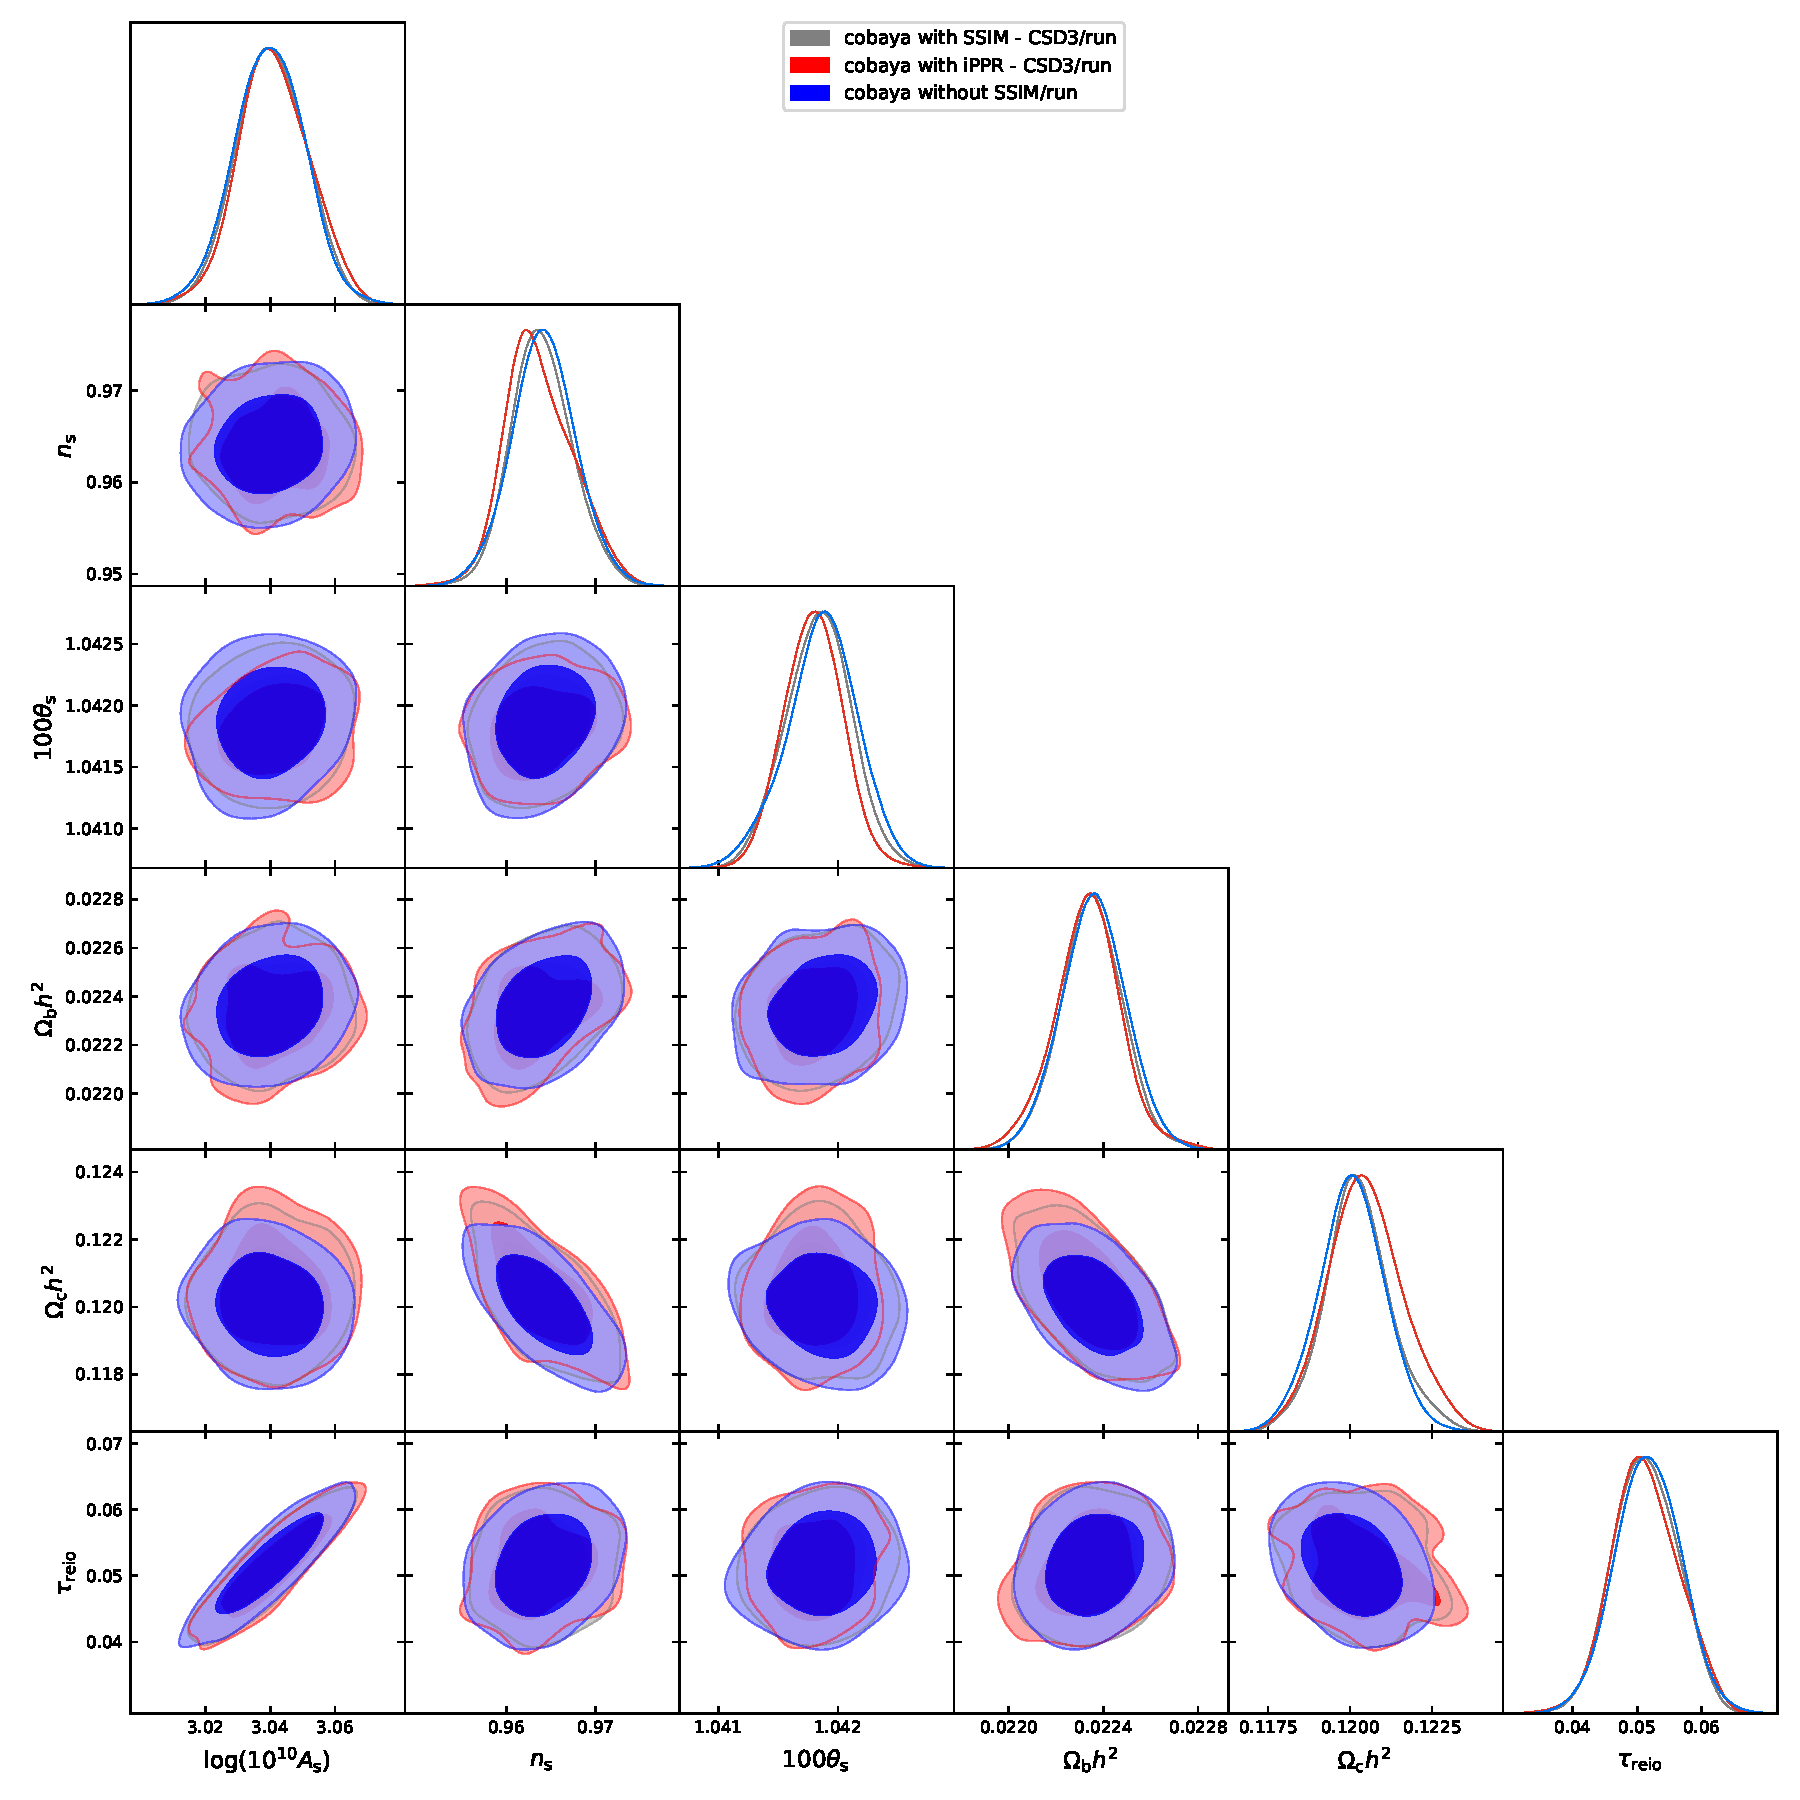
\includegraphics[height=0.95\textheight]{./illustrations/cosmology.pdf}
  \caption{The marginalised posteriors for \texttt{Cobaya} +
    \texttt{Class} on CSD3 with \(n_\text{live}=100\). The Reference
    uniform is \color{red} red \color{black}, while SSIM is
    \color{blue} blue \color{black}. With the exception of
    \(n_\mathrm{s}\) and \(\Omega_\mathrm{c}\), all parameters are
    more tightly constrained. iPPR added to rule out finite-grain-size
    effects for partially representative
    priors. } \label{fig:cosmology}
\end{figure}
\end{landscape}
\begin{landscape}
\begin{figure}
  \centering % Center table
  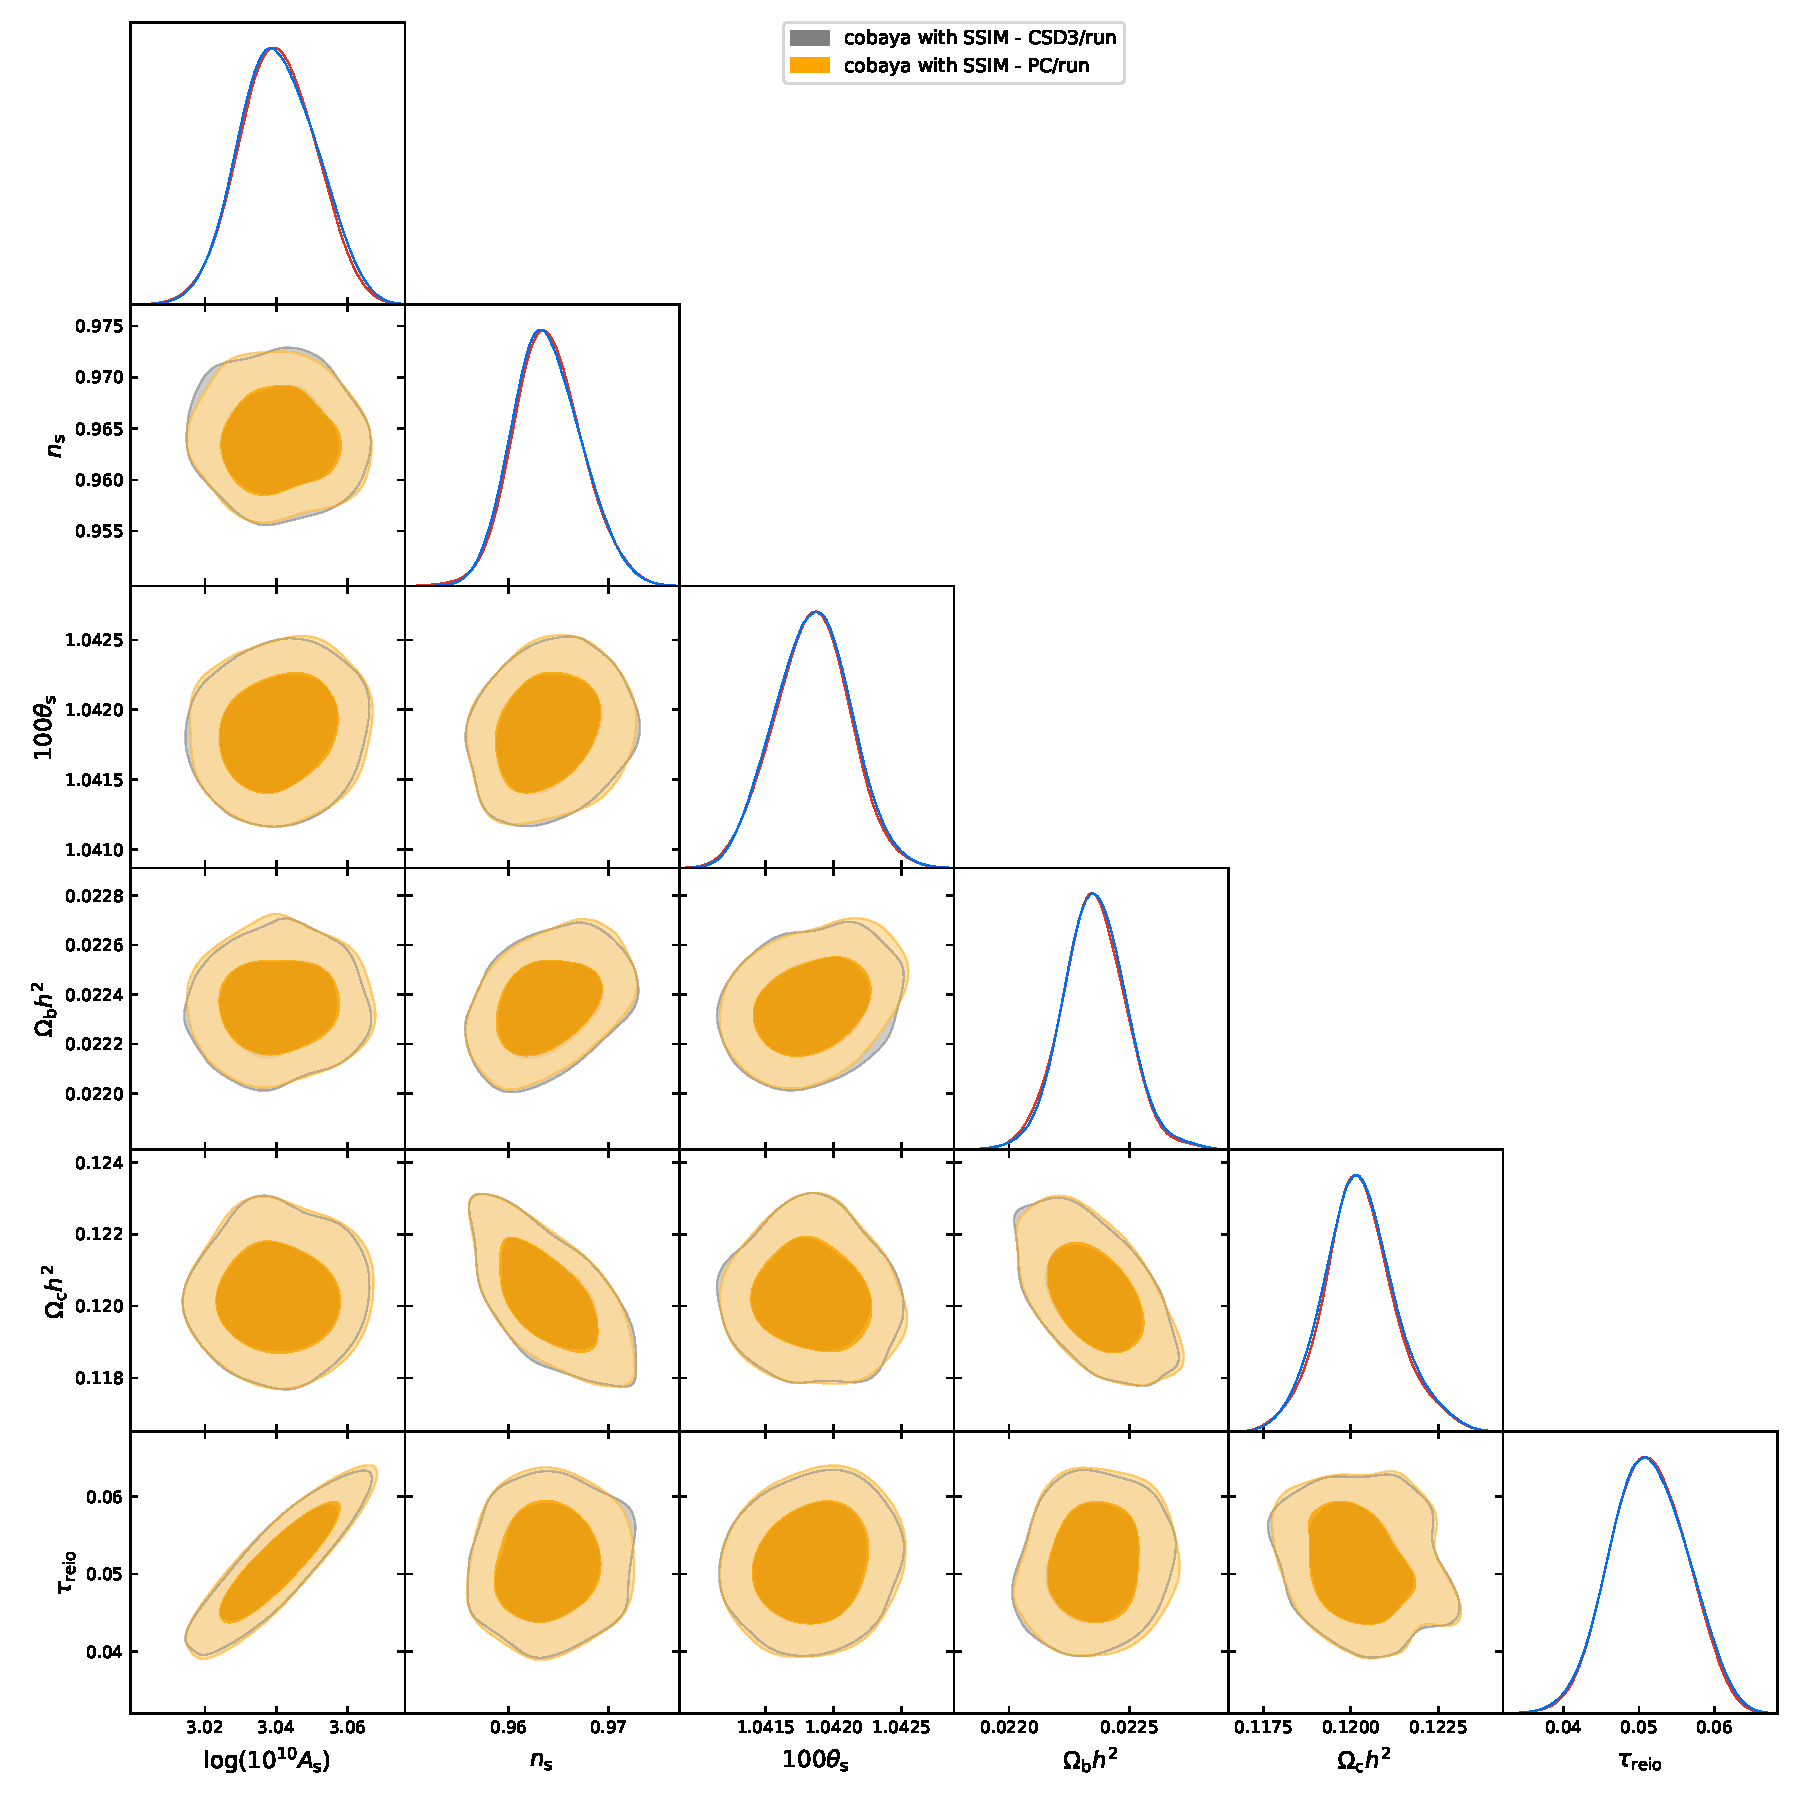
\includegraphics[height=0.95\textheight]{./illustrations/cosmo-pc.pdf}
  \caption{The marginalised posteriors for \texttt{Cobaya} +
    \texttt{Class} on CSD3 with \(n_\text{live}=100\) vs PC
    \(n_\text{live}=50\). } \label{fig:cosmology-pc}
\end{figure}
\end{landscape}





% \section{Nested sampling in detail}\label{sec:ns}
% Consider without loss of generality, a prior space \(\Psi\) that is a
% unit hypercube, where \(\pi(\bm{\theta}) = \text{Const.}\) Draw
% \(n_\text{live}\) random \emph{live points} from the unit
% hypercube. If \({\cal L}\) is a well-behaved function, the probability
% that two points have the same likelihood is vanishing, so each of them
% lies on a \textbf{distinct} iso-likelihood
% hyper-surface\footnote{analogy: height on a contour map. }. Each
% hyper-surface encloses the fraction
% \begin{equation}
% \cfrac{1}{n_\text{live}},
% \end{equation}
% of the total volume of the hypercube on average. More specifically,
% each shell's enclosed volume shall have some random deviation \(\Delta\), from
% \(\cfrac{1}{n_\text{live}}\), with an associated cumulative
% distribution \(P(\Delta)\).

% Subsequently, we pick another point at random, requiring that the
% likelihood of the new point be higher than the lowest likelihood of
% the initial \emph{live point} ensemble. In \citeauthor{Skilling2006}'s
% notation, the point with the lowest likelihood becomes \emph{dead} and
% the new point becomes is \emph{live}. This is a single iteration of
% nested sampling.

% Our argument of approximately equal volumes holds for the new
% ensemble, so the volume encased in the outer-most shell iteratively
% reduces by the same fraction, allows us to approximate said volumes:
% \begin{equation}\label{eq:recurrence-relation}
%   \begin{array}{rcl}
%   X_{0} &=  &1, \\
%   X_{1} &= &X_{0} \left(1- \cfrac{1}{n_\text{live}}\right),\\
%   & \vdots &, \\
%   X_{i} &= &X_{i-1}\left(1- \cfrac{1}{n_\text{live}}\right),\\
%   & \vdots, &
% \end{array}
% \end{equation}
% Thus we iteratively pick live points in regions $\{\bm{\theta}\}$ of
% high \({\cal L}\), and also estimating the evidence, and stop when the
% prior volume encased in the outer shell is lower than a predetermined
% fraction e.g: \(0.01\) of the original hypercube volume.

% The recurrence relation~\eqref{eq:recurrence-relation} is not exact,
% however, \(P(\Delta)\) is a known distribution, dependent on the
% \(\dim \Psi\) and \({\cal L}\). Thus, for each \(\epsilon>0\), there
% exists \(\delta(\epsilon) >0,\) such that
% \(P(\Delta > \delta)<\epsilon.\) Hence, by choosing \(\epsilon\) based
% on \(n_\text{live}\), one obtains an estimate of the error
% \(\delta\). Propagating these errors allows us to evaluate the prior
% volume, ergo: ${\cal Z}$ up to an estimable error.

% This is generalised to non-hypercube $\Psi$ and non-uniform $\pi$ via
% the prior quantile.

% \section{Re-sizeable-bounds uniform prior}\label{sec:resizeable}
% In this appendix, we shall highlight why posterior repartitioning is a
% misnomer, and why the more general idea of evidence repartitioning is
% more fruitful.

% As noted in section~\vref{domain-discussion}, the domains of all
% functions need to be consistent, otherwise~\vref{eq:bayes} no longer
% holds. The mathematical implications of neglecting function domains in
% the context of Quantum mechanics has been discussed
% by~\cite{Gieres_2000}. However, this does not preclude us from
% considering re-parametrisations of $\pi$ and ${\cal L}$ that are
% consistent with the same evidence. 

% To illustrate, consider a uniform prior with the following
% parametrisation:
% \begin{equation}
%   \hat{\pi}(\bm{\theta}; \beta) = \TopHat(\bm{\theta}; \beta \bm{a}, \beta \bm{b}).
% \end{equation}
% Although there are no issues when \(\beta>1\) (we set
% \({\cal\hat{L}}(\bm{\theta}; \beta>1)=0\)), one can immediately
% spot the issues with \(\beta \in (0,1)\); and \(\beta=0\) is
% altogether nonsensical.

% This issue indicates that the prescription of keeping
% \begin{equation}
%   \pi {\cal L} = \text{Const.}
% \end{equation}
% is not complete. Nevertheless, such a scheme may be salvaged if
% \cref{eq:partitioning} is taken as the primary, with counter-intuitive
% extensions, e.g.~for a point \(\bm{\theta}_{0} \notin \Psi\), we don't
% expect
% \begin{equation}
% {\cal L}(\bm{\theta}_{0}) \rightarrow \infty,
% \end{equation}
% but as we shall see:
%   \begin{equation}
%     {\cal L}(\bm{\theta}_{0}) \rightarrow 0.
%   \end{equation}
  
%   The first crucial step is to recognise that the algorithm draws from
%   a unit hypercube with uniform probability, and that the prior is an
%   artefact of a coordinate transformation which we referred to as the
%   prior quantile.

% Let \(u\) be a point in unit hypercube \(\Psi_{C}\). The quantile
% defines a mapping functionally dependent on the PDF of the prior

% \begin{equation}
%   C(\beta)\lbrace \hat{\pi}\rbrace:u \mapsto \bm{\theta},\label{eq:coordinate-transform}
% \end{equation}

% such that
% the uniform distribution of \(\bm{u}\) leads through
% \(C_{\beta}\{\hat{\pi}\}(\bm{u})\) to a \(\hat{\pi}(\bm{\theta};\beta)\)
% distribution of \(\bm{\theta} \in\Psi(\beta)\).Note that we replaced the
% parametrisation of the function \(\hat{\pi}\) with an explicit
% parametrisation of the coordinate transformation, specifically
% \begin{equation}
%   \pi(C(\beta)\{\hat{\pi}\}(u)) \equiv \hat{\pi}(\bm{\theta}; \beta),
% \end{equation}
% where 
% \begin{equation}
%   \hat{\pi} =  \pi \circ C(\beta) \{ \pi \} 
% \end{equation}
% is a parameterised distribution resulting from a parameterised
% coordinate transformation of an un-parameterised prior PDF. We shall
% have~\vref{eq:bayes} hold only in the hypercube
% \begin{equation}
% {\cal \hat{P}}(u) = {\cal P}(C(\beta_{0}){\hat{\pi}}^{-1}(\bm{\theta})) = \cfrac{\hat{\pi} (u) {\cal \hat{L}}(u)}{\int_{\Psi}{\cal \hat{L}}(u) \hat{\pi}(u) du},
% \end{equation}
% which is always true, regardless of the repartitioning
% scheme. Trivially, the functional form of \(P(\bm{\theta})\) is not the same
% as \(P(u)\); it's related via a co-ordinate transform, which in our
% case contributes a Jacobian factor \(J(\beta)\{\hat{\pi}\}\) to the
% evidence. But since we're interested in the posterior in the
% coordinates \(\bm{\theta}\), given by the transformation \(C(\beta_{0})\{\hat{\pi}\}\),
% while the prior and the likelihood are in the from corresponding
% to \(\beta\).

% Finally, 
% \begin{equation}
%  {\cal P}(\bm{\theta}) = \cfrac{J(\beta_{0})}{J(\beta)} \cfrac{\pi(\bm{\theta}; \beta) {\cal L}(\bm{\theta}; \beta)}{\int \pi(\bm{\theta}; \beta) {\cal L}(\bm{\theta}; \beta) d \bm{\theta}}.
% \end{equation}
% So we expect that for the simple case of scaling the uniform box
% prior with \(\beta\), that we need to re-scale the likelihood by
% \(\beta^{2n}\). The second Jacobian factor enters the likelihood because
% we have normalised \(\pi(\bm{\theta})\), but not \(\pi(\bm{\theta}; \beta)\). This is hinted at in
% the notation, (no tilde), and when accounted for, gives  the correct
% posterior and evidence as seen in the experiments.

% \subsubsection{Argument resizing}\label{sec:orgfe92f25}

% A class of convenient repartitioning schemes is one where the prior's
% argument is re-sized e.g:
% \begin{equation}
%   \label{eq:argument-resize}
%   \hat{\pi} (\bm{\theta}; \beta) = \pi (f(\beta)\cdot\bm{\theta}),
% \end{equation}
% where \(f(\beta)\) is some function.

% These are quite convenient as the quantile is straightforwardly
% related to the quantile of the original:
% \begin{equation}
%   \label{eq:quantile-stuff}
%   C\{\hat{\pi}\} = f(\beta) C\{\frac{\pi}{f(\beta)}\}.
% \end{equation}
% We're already acquainted with an exemplar from this class: PPR if
% \( \pi (\bm{\theta}) \propto \exp [P_{n}(\theta)]\) where $P_{n}$ is a
% polynomial.


% \section{Objectivity\label{sec:objectivity}}
% We shall elaborate here on the meaning of \cref{obj-prop}, and why
% \cref{eq:partitioning} and \cref{eq:bayes}, don't guarantee the
% correct \( {\cal P}(\bm{\theta})\) and ${\cal Z}$.  It is a
% peculiarity of nested sampling. It is much faster than e.g.~uniform
% rasterisation, because instead of evaluating ${\cal Z}$ exactly, it
% uses a statistical argument to successively approximate ${\cal
%   Z}$. The four properties are necessary for errors in ${\cal Z}$ to
% accumulate more slowly than is necessary to have moved all of the live
% points onto the posterior peak(s). In \cref{fig:convergence}, we see a
% particular case that highlights what happens if \cref{obj-prop} is
% violated.

% Specifically, the arrangement of prior and posterior is such that
% points lie in regions of average likelihood. Along the $\theta_{1}$
% direction, the likelihood is so large that any small displacement
% within the prior in the direction of the posterior accounts for a
% large portion of the evidence. This is seen in \cref{fig:higson},
% where the bulk of the evidence is gathered early.

% However, along $\theta_{3}$ there is a significant difference in the
% likelihood, so a small fraction of the live points do indeed get moved
% onto the posterior. Nonetheless, we reached the termination criterion
% before points could have been moved fully, producing an incorrect
% marginalised posterior.  This situation is contrived, as it required
% fine-tuning. The odds of this occurring in practice are minuscule, and
% the presence of \cref{fig:convergence} does not invalidate the
% importance of PPR.


% This highlights a crucial problem with PPR (and later, additive
% mixtures) that the probability of having an unbiased prior in some
% region is negligible\footnote{ \(P(\beta=0)\) to be precise.}. There
% is always a bias: points are always more likely to spawn and be moved
% towards the prior peak. When using repartitioning, we need to ensure
% that this bias is weaker than the bias towards the posterior. The
% latter is implementation-dependent, \texttt{MultiNest} is more prone
% to such errors.

% However, crucially, we will have obtained a smaller evidence with a
% larger error: this is the only way in which the posterior may appear
% the way it does in \cref{fig:convergence} without violating
% \cref{eq:bayes}. Corollary: we will have known if the posterior is
% dubious. In \cref{sec:results}, we discussed how to proceed should
% such a scenario arise.

% \section{Making PPR robust again}
% The shortcomings of PPR, may be somewhat mitigated if the goal is to
% ensure stable convergence, rather than maximally improving
% performance. Start by noting that $\beta$ according to nested sampling
% is nothing but an extra nuisance parameter: it requires a prior. This
% prior plays a pivotal role in PPR's stability. In fact there is an
% obvious, maximally stable, choice:
% \begin{equation}
%   \label{}
% \hat{\pi}(\bm{\theta}; \beta) = \delta(\beta) \hat{\pi}(\bm{\theta}), 
% \end{equation}
% which is exactly the uniform prior. It is unbiased: any region inside
% the boundaries, and excluding the boundaries is equally likely to be
% sampled. This is because $\pi^{\beta}(\bm{\theta})$ is uniform, when $\beta=0$, and
% \begin{equation}\label{eq:PPR-uniform}
% P(\beta=0) = \int_{\mathbb{R}} \delta(\beta) d\beta = 1 \ne 0. 
% \end{equation}
% By adding extra $\delta$-functions we can simulate a fixed Stochastic
% isometric superposition. Similarly, by allowing the weights of these
% $\delta$-functions to vary, we can simulate a superpositional
% isometric mixture of priors related by power law, e.g.
% \begin{equation}
%   \label{}
%   \hat{\pi}(\beta; \bm{w}) = w_{0}\delta(\beta_{0}) + w_{1}\delta(\beta_{1})+\ldots
% \end{equation}
% These are known to be more robust than PPR alone, so a choice of
% $\hat{\pi}(\beta)$ that makes PPR distinct and useful should exist.

% A clue lies in that $\beta=0$ is special. So a sensible next step
% would be to try
% \begin{equation}
%   \label{}
% \hat{\pi}(\beta; w) = w \delta(\beta) + (1-w). 
% \end{equation}
% This is equivalent to a uniform $\beta$ PPR (\(1-w\) in a stochastic
% mixture with a uniform prior ($\delta(\beta)$). In general the second
% term can be any function, and it would still be a superpositional
% mixture of PPR with that function as the prior in $\beta$ and a
% uniform.

% What about
% \begin{equation}
% \hat{\pi}(\beta; \sigma) = G(\beta; 0, \sigma)?
% \end{equation}
% For numerical simulations, it has some probability (dependent on
% $\sigma \ne 0$) to be unbiased. It is weakly biased, as
% \(P(\beta=0) \rightarrow 0\) with increasing resolution:
% \begin{equation}
%   \label{eq:p0}
%    P(\beta=0) = \lim_{\epsilon\rightarrow 0} \int_{-\epsilon}^{\epsilon}\hat{\pi}(\beta) = 0
% \end{equation}
% but it is already an improvement over a uniform prior (in $\beta$).

% Sadly, \cref{eq:p0} highlights why priors $\hat{\pi}(\beta)$ can never
% outperform SSIM in producing an unbiased prior. If
% $\hat{\pi}(\bm{\theta}, \beta)$ is such that \(P(\beta=0) = w \ne 0\)
% it is equivalent to a superpositional isometric mixture of uniform
% (with weight \(w\)) and a PPR with prior
% $\tilde{\pi}(\beta) = \hat{\pi}(\beta) - w \delta(\beta)$.

% So, superpositional mixtures can be implemented using PPR by varying
% the prior in $\beta$.










\end{document}
